% Options for packages loaded elsewhere
\PassOptionsToPackage{unicode}{hyperref}
\PassOptionsToPackage{hyphens}{url}
\PassOptionsToPackage{dvipsnames,svgnames,x11names}{xcolor}
%
\documentclass[
  letterpaper,
  DIV=11,
  numbers=noendperiod]{scrreprt}

\usepackage{amsmath,amssymb}
\usepackage{iftex}
\ifPDFTeX
  \usepackage[T1]{fontenc}
  \usepackage[utf8]{inputenc}
  \usepackage{textcomp} % provide euro and other symbols
\else % if luatex or xetex
  \usepackage{unicode-math}
  \defaultfontfeatures{Scale=MatchLowercase}
  \defaultfontfeatures[\rmfamily]{Ligatures=TeX,Scale=1}
\fi
\usepackage{lmodern}
\ifPDFTeX\else  
    % xetex/luatex font selection
\fi
% Use upquote if available, for straight quotes in verbatim environments
\IfFileExists{upquote.sty}{\usepackage{upquote}}{}
\IfFileExists{microtype.sty}{% use microtype if available
  \usepackage[]{microtype}
  \UseMicrotypeSet[protrusion]{basicmath} % disable protrusion for tt fonts
}{}
\makeatletter
\@ifundefined{KOMAClassName}{% if non-KOMA class
  \IfFileExists{parskip.sty}{%
    \usepackage{parskip}
  }{% else
    \setlength{\parindent}{0pt}
    \setlength{\parskip}{6pt plus 2pt minus 1pt}}
}{% if KOMA class
  \KOMAoptions{parskip=half}}
\makeatother
\usepackage{xcolor}
\setlength{\emergencystretch}{3em} % prevent overfull lines
\setcounter{secnumdepth}{4}
% Make \paragraph and \subparagraph free-standing
\ifx\paragraph\undefined\else
  \let\oldparagraph\paragraph
  \renewcommand{\paragraph}[1]{\oldparagraph{#1}\mbox{}}
\fi
\ifx\subparagraph\undefined\else
  \let\oldsubparagraph\subparagraph
  \renewcommand{\subparagraph}[1]{\oldsubparagraph{#1}\mbox{}}
\fi


\providecommand{\tightlist}{%
  \setlength{\itemsep}{0pt}\setlength{\parskip}{0pt}}\usepackage{longtable,booktabs,array}
\usepackage{calc} % for calculating minipage widths
% Correct order of tables after \paragraph or \subparagraph
\usepackage{etoolbox}
\makeatletter
\patchcmd\longtable{\par}{\if@noskipsec\mbox{}\fi\par}{}{}
\makeatother
% Allow footnotes in longtable head/foot
\IfFileExists{footnotehyper.sty}{\usepackage{footnotehyper}}{\usepackage{footnote}}
\makesavenoteenv{longtable}
\usepackage{graphicx}
\makeatletter
\def\maxwidth{\ifdim\Gin@nat@width>\linewidth\linewidth\else\Gin@nat@width\fi}
\def\maxheight{\ifdim\Gin@nat@height>\textheight\textheight\else\Gin@nat@height\fi}
\makeatother
% Scale images if necessary, so that they will not overflow the page
% margins by default, and it is still possible to overwrite the defaults
% using explicit options in \includegraphics[width, height, ...]{}
\setkeys{Gin}{width=\maxwidth,height=\maxheight,keepaspectratio}
% Set default figure placement to htbp
\makeatletter
\def\fps@figure{htbp}
\makeatother
% definitions for citeproc citations
\NewDocumentCommand\citeproctext{}{}
\NewDocumentCommand\citeproc{mm}{%
  \begingroup\def\citeproctext{#2}\cite{#1}\endgroup}
\makeatletter
 % allow citations to break across lines
 \let\@cite@ofmt\@firstofone
 % avoid brackets around text for \cite:
 \def\@biblabel#1{}
 \def\@cite#1#2{{#1\if@tempswa , #2\fi}}
\makeatother
\newlength{\cslhangindent}
\setlength{\cslhangindent}{1.5em}
\newlength{\csllabelwidth}
\setlength{\csllabelwidth}{3em}
\newenvironment{CSLReferences}[2] % #1 hanging-indent, #2 entry-spacing
 {\begin{list}{}{%
  \setlength{\itemindent}{0pt}
  \setlength{\leftmargin}{0pt}
  \setlength{\parsep}{0pt}
  % turn on hanging indent if param 1 is 1
  \ifodd #1
   \setlength{\leftmargin}{\cslhangindent}
   \setlength{\itemindent}{-1\cslhangindent}
  \fi
  % set entry spacing
  \setlength{\itemsep}{#2\baselineskip}}}
 {\end{list}}
\usepackage{calc}
\newcommand{\CSLBlock}[1]{\hfill\break\parbox[t]{\linewidth}{\strut\ignorespaces#1\strut}}
\newcommand{\CSLLeftMargin}[1]{\parbox[t]{\csllabelwidth}{\strut#1\strut}}
\newcommand{\CSLRightInline}[1]{\parbox[t]{\linewidth - \csllabelwidth}{\strut#1\strut}}
\newcommand{\CSLIndent}[1]{\hspace{\cslhangindent}#1}

\KOMAoption{captions}{tableheading}
\makeatletter
\@ifpackageloaded{bookmark}{}{\usepackage{bookmark}}
\makeatother
\makeatletter
\@ifpackageloaded{caption}{}{\usepackage{caption}}
\AtBeginDocument{%
\ifdefined\contentsname
  \renewcommand*\contentsname{Tabla de contenidos}
\else
  \newcommand\contentsname{Tabla de contenidos}
\fi
\ifdefined\listfigurename
  \renewcommand*\listfigurename{Listado de Figuras}
\else
  \newcommand\listfigurename{Listado de Figuras}
\fi
\ifdefined\listtablename
  \renewcommand*\listtablename{Listado de Tablas}
\else
  \newcommand\listtablename{Listado de Tablas}
\fi
\ifdefined\figurename
  \renewcommand*\figurename{Figura}
\else
  \newcommand\figurename{Figura}
\fi
\ifdefined\tablename
  \renewcommand*\tablename{Tabla}
\else
  \newcommand\tablename{Tabla}
\fi
}
\@ifpackageloaded{float}{}{\usepackage{float}}
\floatstyle{ruled}
\@ifundefined{c@chapter}{\newfloat{codelisting}{h}{lop}}{\newfloat{codelisting}{h}{lop}[chapter]}
\floatname{codelisting}{Listado}
\newcommand*\listoflistings{\listof{codelisting}{Listado de Listados}}
\makeatother
\makeatletter
\makeatother
\makeatletter
\@ifpackageloaded{caption}{}{\usepackage{caption}}
\@ifpackageloaded{subcaption}{}{\usepackage{subcaption}}
\makeatother
\ifLuaTeX
\usepackage[bidi=basic]{babel}
\else
\usepackage[bidi=default]{babel}
\fi
\babelprovide[main,import]{spanish}
% get rid of language-specific shorthands (see #6817):
\let\LanguageShortHands\languageshorthands
\def\languageshorthands#1{}
\ifLuaTeX
  \usepackage{selnolig}  % disable illegal ligatures
\fi
\usepackage{bookmark}

\IfFileExists{xurl.sty}{\usepackage{xurl}}{} % add URL line breaks if available
\urlstyle{same} % disable monospaced font for URLs
\hypersetup{
  pdftitle={Reporte ID23\_10297},
  pdfauthor={M. Abel Herrera},
  pdflang={es},
  colorlinks=true,
  linkcolor={blue},
  filecolor={Maroon},
  citecolor={Blue},
  urlcolor={Blue},
  pdfcreator={LaTeX via pandoc}}

\title{Reporte ID23\_10297}
\author{M. Abel Herrera}
\date{Invalid Date}

\begin{document}
\maketitle

\renewcommand*\contentsname{Tabla de contenidos}
{
\hypersetup{linkcolor=}
\setcounter{tocdepth}{2}
\tableofcontents
}
\bookmarksetup{startatroot}

\chapter*{Preface}\label{preface}
\addcontentsline{toc}{chapter}{Preface}

\markboth{Preface}{Preface}

This is a Quarto book.

To learn more about Quarto books visit
\url{https://quarto.org/docs/books}.

\begin{verbatim}
[1] 2
\end{verbatim}

\bookmarksetup{startatroot}

\chapter{Introduction}\label{introduction}

This is a book created from markdown and executable code.

See Knuth (1984) for additional discussion of literate programming.

\begin{verbatim}
[1] 2
\end{verbatim}

\bookmarksetup{startatroot}

\chapter{Summary}\label{summary}

In summary, this book has no content whatsoever.

\begin{verbatim}
[1] 2
\end{verbatim}

\part{Capítulo 1: Análisis explotatorio}

\chapter{Producción}\label{producciuxf3n}

Aquí vendría el texto sobre la producción y la metodología sobre la toma
de muestras.

\section{Peso total}\label{peso-total}

\begin{center}
\includegraphics{0101_produccion_files/figure-pdf/unnamed-chunk-2-1.pdf}
\end{center}

\section{Rendimiento}\label{rendimiento}

Considerando el área de influencia de cada árbol como 8 m2, el
rendimiento se determinó dividiendo el peso total de la producción del
árbol entre su área de influencia en hectareas (0.0008 ha).

\begin{center}
\includegraphics{0101_produccion_files/figure-pdf/unnamed-chunk-3-1.pdf}
\end{center}

\section{Densidad}\label{densidad}

Para estimar la densidad de la producción, se tomó una muestra aleatoria
de 1 kg de la producción total del árbol. Posteriormente se
contabilizaron los frutos de aquella muestra para obtener la densidad
como la cantidad de frutos por kilogramo.

\begin{center}
\includegraphics{0101_produccion_files/figure-pdf/unnamed-chunk-4-1.pdf}
\end{center}

\chapter{Calidad}\label{calidad}

Aquí vendría el texto sobre la calidad y la metodología sobre la toma de
muestras.

\section{Apariencia}\label{apariencia}

La apariencia de los frutos se evaluó considerando su peso, diámetro y
color. Para llevar a cabo este análisis, se seleccionaron al azar 20
frutos de una muestra representativa equivalente a 1 kg de la producción
total.

\subsection{Peso}\label{peso}

\begin{center}
\includegraphics{0102_calidad_files/figure-pdf/unnamed-chunk-3-1.pdf}
\end{center}

\subsection{Diametro}\label{diametro}

\begin{center}
\includegraphics{0102_calidad_files/figure-pdf/unnamed-chunk-4-1.pdf}
\end{center}

\subsection{Color}\label{color}

Para cuantificar y calificar el color dentro de las muestras, se
categorizó el color de cada fruto como se muestra en la
Figura~\ref{fig-escala}.

\begin{figure}

\centering{

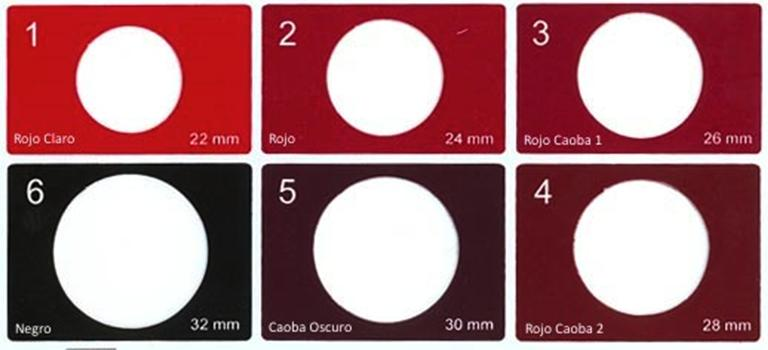
\includegraphics{figuras/misc/10_tabla_de_color.jpg}

}

\caption{\label{fig-escala}Escala de color de cerezas.}

\end{figure}%

\begin{center}
\includegraphics{0102_calidad_files/figure-pdf/unnamed-chunk-5-1.pdf}
\end{center}

\section{Contenido de azucar}\label{contenido-de-azucar}

Para determinar el contenido de azúcar, se midieron los grados Brix de
cada fruto mediante la utilización de un refractrometro. Los frutos
utilizados correspondieron a cinco frutos de cada árbol escogidos al
azar, a partir de una selección de frutos de buena apariencia dentro de
la muestra de 1 kg.

\begin{center}
\includegraphics{0102_calidad_files/figure-pdf/unnamed-chunk-6-1.pdf}
\end{center}

\section{Daño}\label{dauxf1o}

Para determinar el daño de la producción, se estimó el porcentaje de
frutos dañados a partir de una muesrtra aleatoria de 1 kg de la
producción total. Los frutos dañados se consideraron como aquellos que
presentaban desde daños severos o de la marchitez total del fruto hasta
cracking leves, además de frutos dobles.

\begin{center}
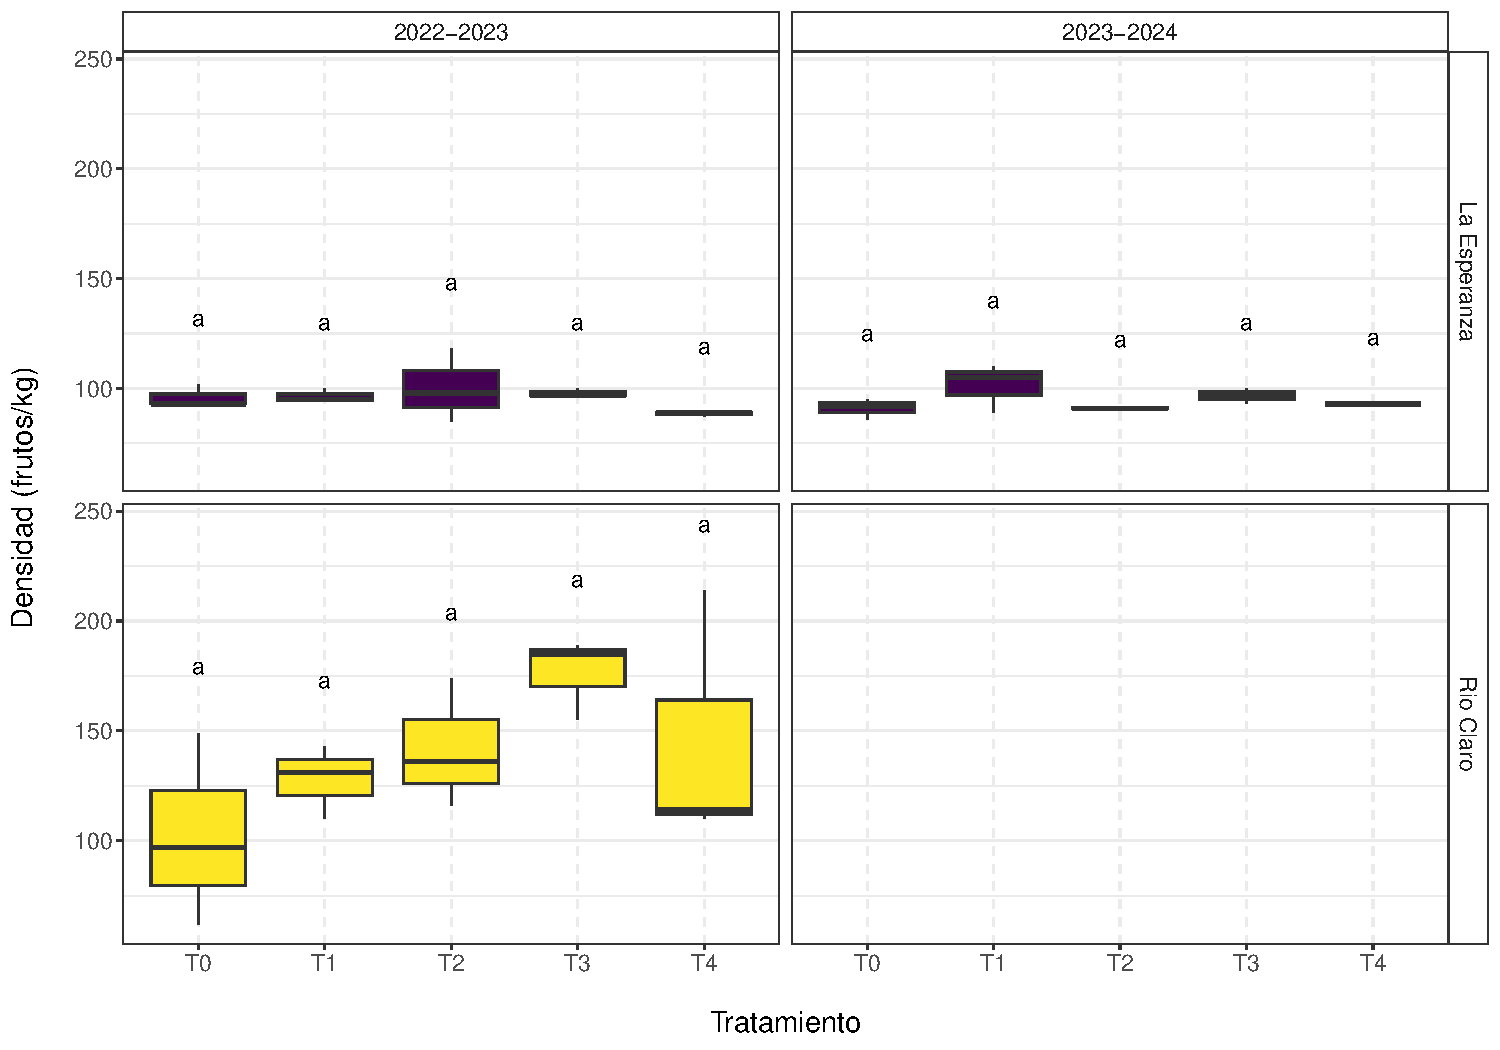
\includegraphics{0102_calidad_files/figure-pdf/unnamed-chunk-7-1.pdf}
\end{center}

\chapter{Parámetros fisiológicos}\label{paruxe1metros-fisioluxf3gicos}

\section{Fluorescencia}\label{fluorescencia}

Los datos de fluorescencia han sido recopilados mediante el uso de
fluorómetro FluorPen (FUENTE), entre 13:00 y 14:00 de forma semanal, en
ambos sitios para la temporada 2022-2023 y 2023-2024.

El índice utilizado es el Rendimiento Cuántico Máximo del Fotosistema II
(ΦP0).

\chapter{Distribución}

\begin{center}
\includegraphics{0103_parametros_files/figure-pdf/unnamed-chunk-2-1.pdf}
\end{center}

\chapter{Serie temporal}

\begin{center}
\includegraphics{0103_parametros_files/figure-pdf/unnamed-chunk-3-1.pdf}
\end{center}

\chapter{Población de datos}

La siguiente tabla presenta la población de datos según temporada,
sitio, tratamiento y unidad.

\begin{longtable}[]{@{}llllr@{}}
\toprule\noalign{}
Temporada & Sitio & Tratamiento & Unidad & n \\
\midrule\noalign{}
\endhead
\bottomrule\noalign{}
\endlastfoot
2022-2023 & La Esperanza & T0 & 1 & 14 \\
& & & 2 & 14 \\
& & & 3 & 14 \\
& & T1 & 1 & 16 \\
& & & 2 & 16 \\
& & & 3 & 16 \\
& & T2 & 1 & 16 \\
& & & 2 & 16 \\
& & & 3 & 16 \\
& & T3 & 1 & 16 \\
& & & 2 & 16 \\
& & & 3 & 16 \\
& & T4 & 1 & 16 \\
& & & 2 & 16 \\
& & & 3 & 16 \\
& Rio Claro & T0 & 1 & 16 \\
& & & 2 & 16 \\
& & & 3 & 16 \\
& & T1 & 1 & 18 \\
& & & 2 & 18 \\
& & & 3 & 18 \\
& & T2 & 1 & 18 \\
& & & 2 & 18 \\
& & & 3 & 18 \\
& & T3 & 1 & 18 \\
& & & 2 & 18 \\
& & & 3 & 18 \\
& & T4 & 1 & 18 \\
& & & 2 & 18 \\
& & & 3 & 18 \\
2023-2024 & La Esperanza & T0 & 1 & 15 \\
& & & 2 & 15 \\
& & & 3 & 15 \\
& & T1 & 1 & 15 \\
& & & 2 & 15 \\
& & & 3 & 15 \\
& & T2 & 1 & 15 \\
& & & 2 & 15 \\
& & & 3 & 15 \\
& & T3 & 1 & 15 \\
& & & 2 & 15 \\
& & & 3 & 15 \\
& & T4 & 1 & 15 \\
& & & 2 & 15 \\
& & & 3 & 15 \\
& Rio Claro & T0 & 1 & 13 \\
& & & 2 & 13 \\
& & & 3 & 13 \\
& & T1 & 1 & 13 \\
& & & 2 & 13 \\
& & & 3 & 13 \\
& & T2 & 1 & 13 \\
& & & 2 & 13 \\
& & & 3 & 13 \\
& & T3 & 1 & 13 \\
& & & 2 & 13 \\
& & & 3 & 13 \\
& & T4 & 1 & 13 \\
& & & 2 & 13 \\
& & & 3 & 13 \\
\end{longtable}

\section{Potencial}\label{potencial}

Los datos de potencial hídrico xilemático han sido recopilados mediante
el uso de una camara de presión o bomba Scholander (FUENTE), entre 13:00
y 14:00 de forma semanal, en ambos sitios para la temporada 2022-2023 y
2023-2024.

\chapter{Distribución}

\begin{center}
\includegraphics{0103_parametros_files/figure-pdf/unnamed-chunk-5-1.pdf}
\end{center}

\chapter{Serie temporal}

\begin{center}
\includegraphics{0103_parametros_files/figure-pdf/unnamed-chunk-6-1.pdf}
\end{center}

\chapter{Población de datos}

La siguiente tabla presenta la población de datos según temporada, sitio
y tratamiento.

\begin{longtable}[]{@{}llllr@{}}
\toprule\noalign{}
Temporada & Sitio & Tratamiento & Unidad & n \\
\midrule\noalign{}
\endhead
\bottomrule\noalign{}
\endlastfoot
2022-2023 & La Esperanza & T0 & 1 & 11 \\
& & & 2 & 11 \\
& & & 3 & 11 \\
& & T1 & 1 & 12 \\
& & & 2 & 12 \\
& & & 3 & 11 \\
& & T2 & 1 & 12 \\
& & & 2 & 12 \\
& & & 3 & 12 \\
& & T3 & 1 & 12 \\
& & & 2 & 12 \\
& & & 3 & 12 \\
& & T4 & 1 & 12 \\
& & & 2 & 12 \\
& & & 3 & 12 \\
& Rio Claro & T0 & 1 & 13 \\
& & & 2 & 13 \\
& & & 3 & 13 \\
& & T1 & 1 & 14 \\
& & & 2 & 14 \\
& & & 3 & 15 \\
& & T2 & 1 & 15 \\
& & & 2 & 14 \\
& & & 3 & 15 \\
& & T3 & 1 & 14 \\
& & & 2 & 14 \\
& & & 3 & 15 \\
& & T4 & 1 & 14 \\
& & & 2 & 14 \\
& & & 3 & 15 \\
2023-2024 & La Esperanza & T0 & 1 & 21 \\
& & & 2 & 21 \\
& & & 3 & 21 \\
& & T1 & 1 & 21 \\
& & & 2 & 20 \\
& & & 3 & 21 \\
& & T2 & 1 & 20 \\
& & & 2 & 21 \\
& & & 3 & 21 \\
& & T3 & 1 & 21 \\
& & & 2 & 21 \\
& & & 3 & 20 \\
& & T4 & 1 & 21 \\
& & & 2 & 20 \\
& & & 3 & 20 \\
& Rio Claro & T0 & 1 & 14 \\
& & & 2 & 13 \\
& & & 3 & 13 \\
& & T1 & 1 & 14 \\
& & & 2 & 14 \\
& & & 3 & 13 \\
& & T2 & 1 & 13 \\
& & & 2 & 13 \\
& & & 3 & 14 \\
& & T3 & 1 & 13 \\
& & & 2 & 13 \\
& & & 3 & 13 \\
& & T4 & 1 & 13 \\
& & & 2 & 13 \\
& & & 3 & 14 \\
\end{longtable}

\subsection{Ciclio diario}\label{ciclio-diario}

Además del valor de potencial único diario que se recopilaba en cierto
rango horario para cada unidad de muestreo, también se realizaron
jornadas de recopilación de valores horarios de potencial a lo largo del
día, con el fin de caracterizar el ciclo diario o perfil horario de este
en las distintas unidades. Estos valores se recopilaron cada una hora
desde las 8 am hasta las 8 pm, mediante la misma metodología que la
extracción del valor único diario pero con menor tiempo de oscuridad y
sellado en las hojas (30 a 45 min).

A continuación se muestran los resultados de la caracterización del
ciclo diario del potencial.

\begin{center}
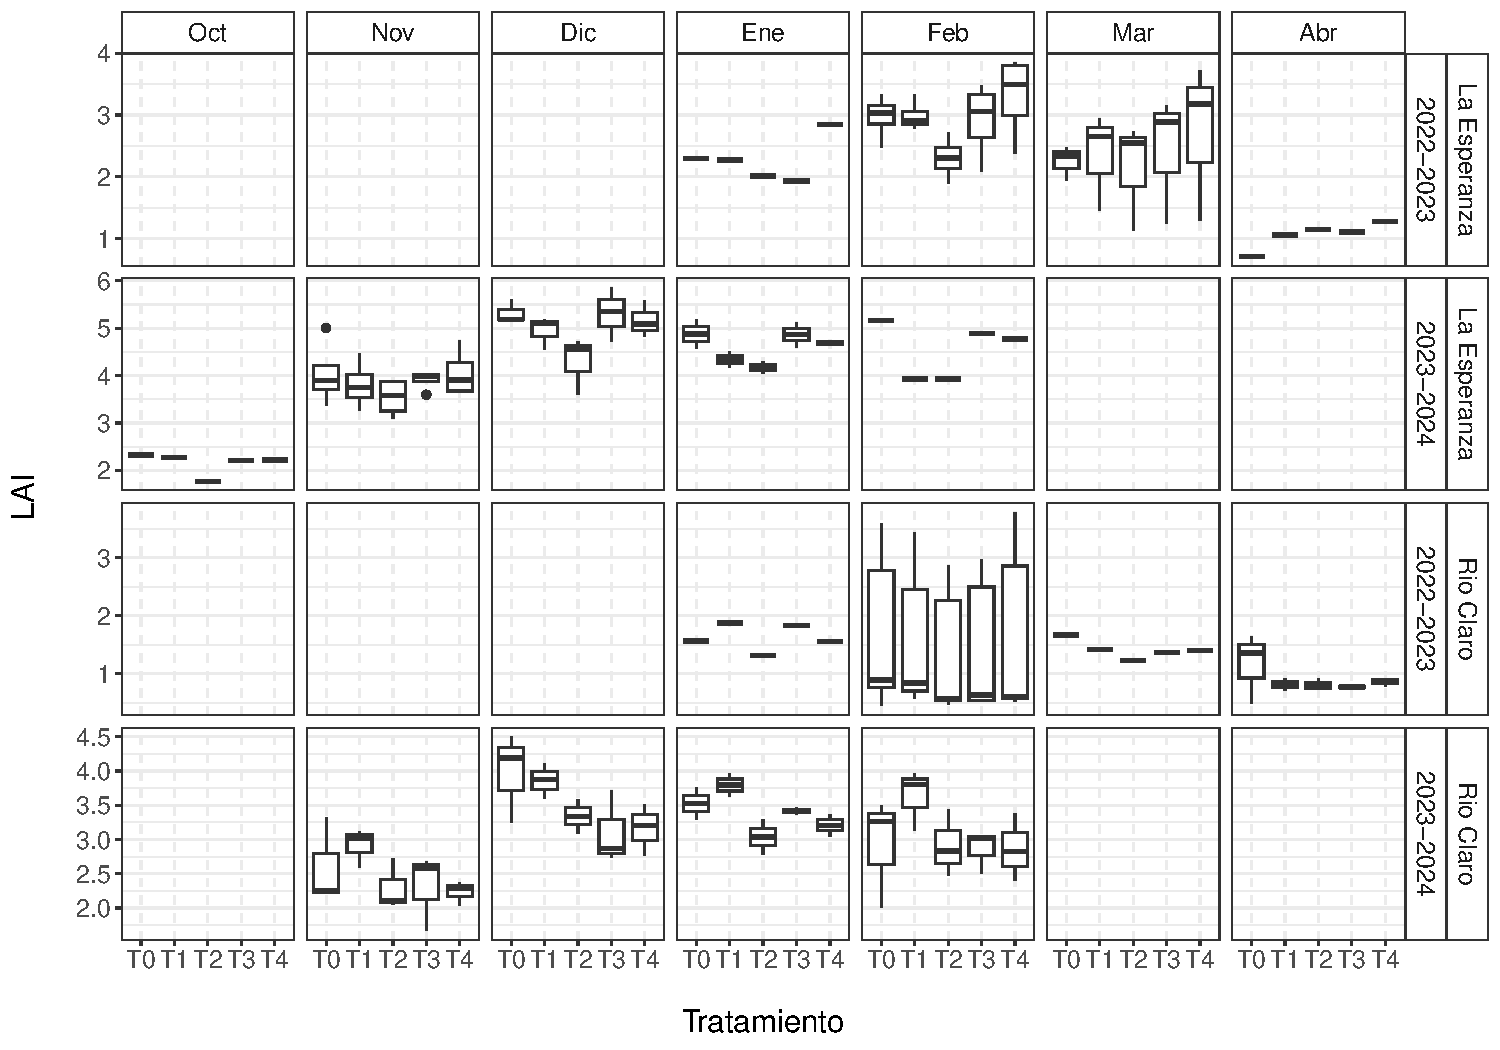
\includegraphics{0103_parametros_files/figure-pdf/unnamed-chunk-8-1.pdf}
\end{center}

\section{LAI}\label{lai}

Los datos de LAI han sido recopilados mediante el uso de ceptometro LP80
(FUENTE), entre 12:30 y 13:30 de forma semanal, en ambos sitios para la
temporada 2022-2023 y 2023-2024.

\chapter{Distribución}

\begin{center}
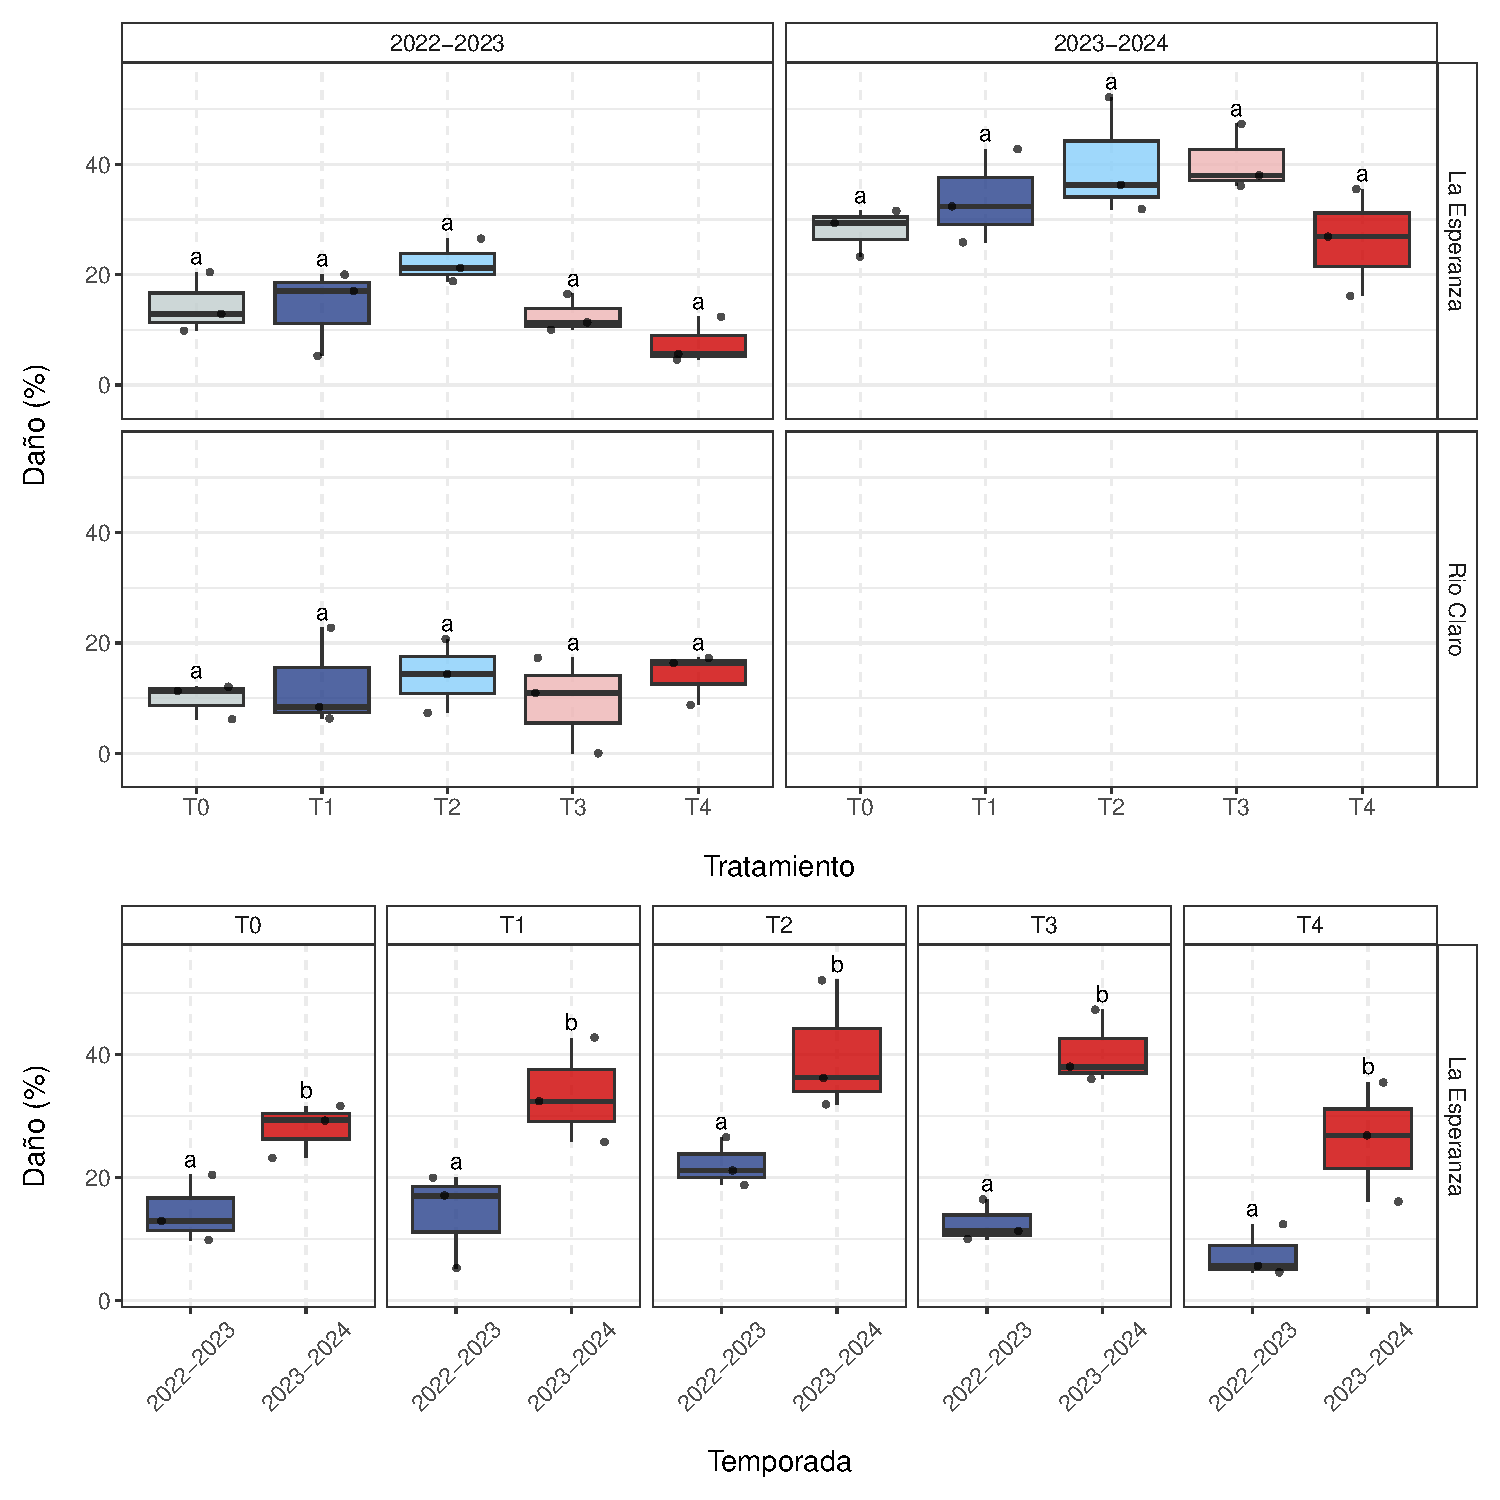
\includegraphics{0103_parametros_files/figure-pdf/unnamed-chunk-9-1.pdf}
\end{center}

\chapter{Serie temporal}

\begin{center}
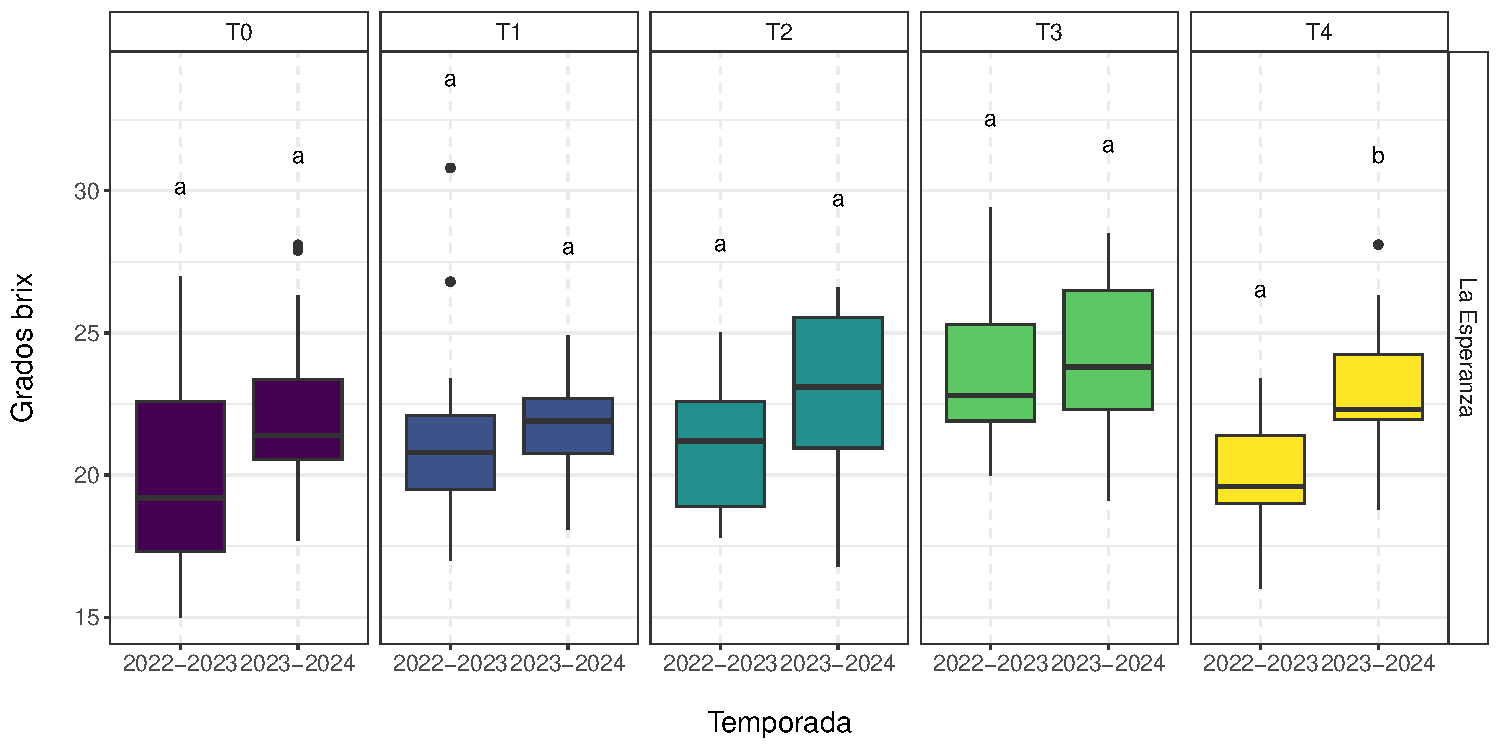
\includegraphics{0103_parametros_files/figure-pdf/unnamed-chunk-10-1.pdf}
\end{center}

\chapter{Población de datos}

La siguiente tabla presenta la población de datos según temporada, sitio
y tratamiento.

\begin{longtable}[]{@{}lllr@{}}
\toprule\noalign{}
Temporada & Sitio & Tratamiento & n \\
\midrule\noalign{}
\endhead
\bottomrule\noalign{}
\endlastfoot
2022-2023 & La Esperanza & T0 & 9 \\
& & T1 & 9 \\
& & T2 & 9 \\
& & T3 & 9 \\
& & T4 & 9 \\
& Rio Claro & T0 & 10 \\
& & T1 & 10 \\
& & T2 & 10 \\
& & T3 & 10 \\
& & T4 & 10 \\
2023-2024 & La Esperanza & T0 & 11 \\
& & T1 & 11 \\
& & T2 & 11 \\
& & T3 & 11 \\
& & T4 & 11 \\
& Rio Claro & T0 & 11 \\
& & T1 & 11 \\
& & T2 & 11 \\
& & T3 & 11 \\
& & T4 & 11 \\
\end{longtable}

\section{Turgor: presión de parche}\label{sec-turgor}

Los datos de turgor han sido recopilados mediante el uso de sensores ZIM
(FUENTE), los cuales miden presión de parche en una determinada hoja
cada media hora de forma continua. Estos fueron dispuestos en cada
unidad de los tratamientos (dos sensores por unidad), en ambos sitios
durante la temporada 2022-2023 y 2023-2024.

En estos datos se observó presencia de ruido, atribuida a factores como
la marchitez de las hojas muestreadas, fuerzas externas que provocaban
el desalineamiento de los imanes del sensor y otras causas que llevaron
a la recalibración de los sensores. Como resultado, se presentan a
continuación tanto los datos crudos, con el ruido presente, como los
datos preprocesados limpios, los cuales han sido depurados de dicho
ruido.

\chapter{Distribución}

\begin{center}
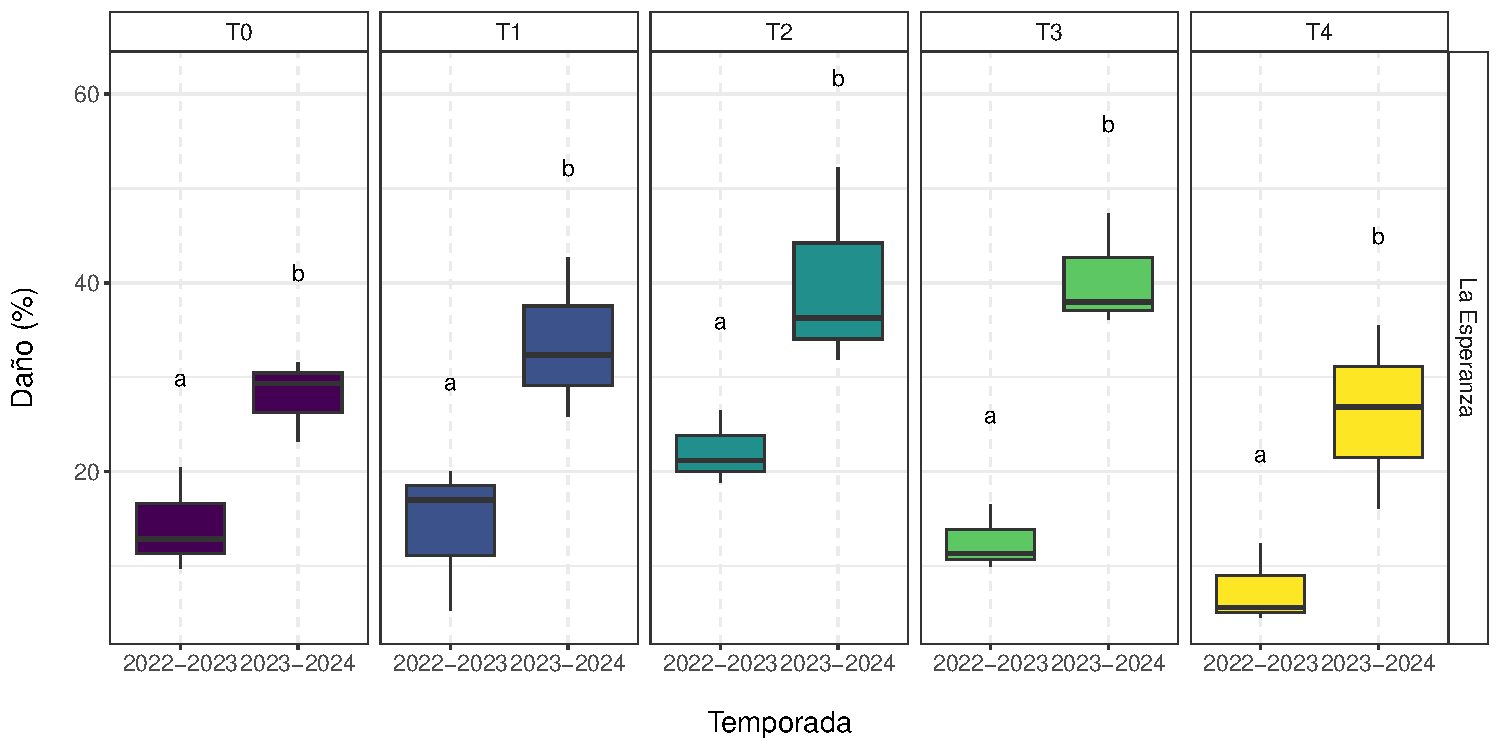
\includegraphics{0103_parametros_files/figure-pdf/unnamed-chunk-12-1.pdf}
\end{center}

\chapter{Serie temporal 2022-2023}

\begin{center}
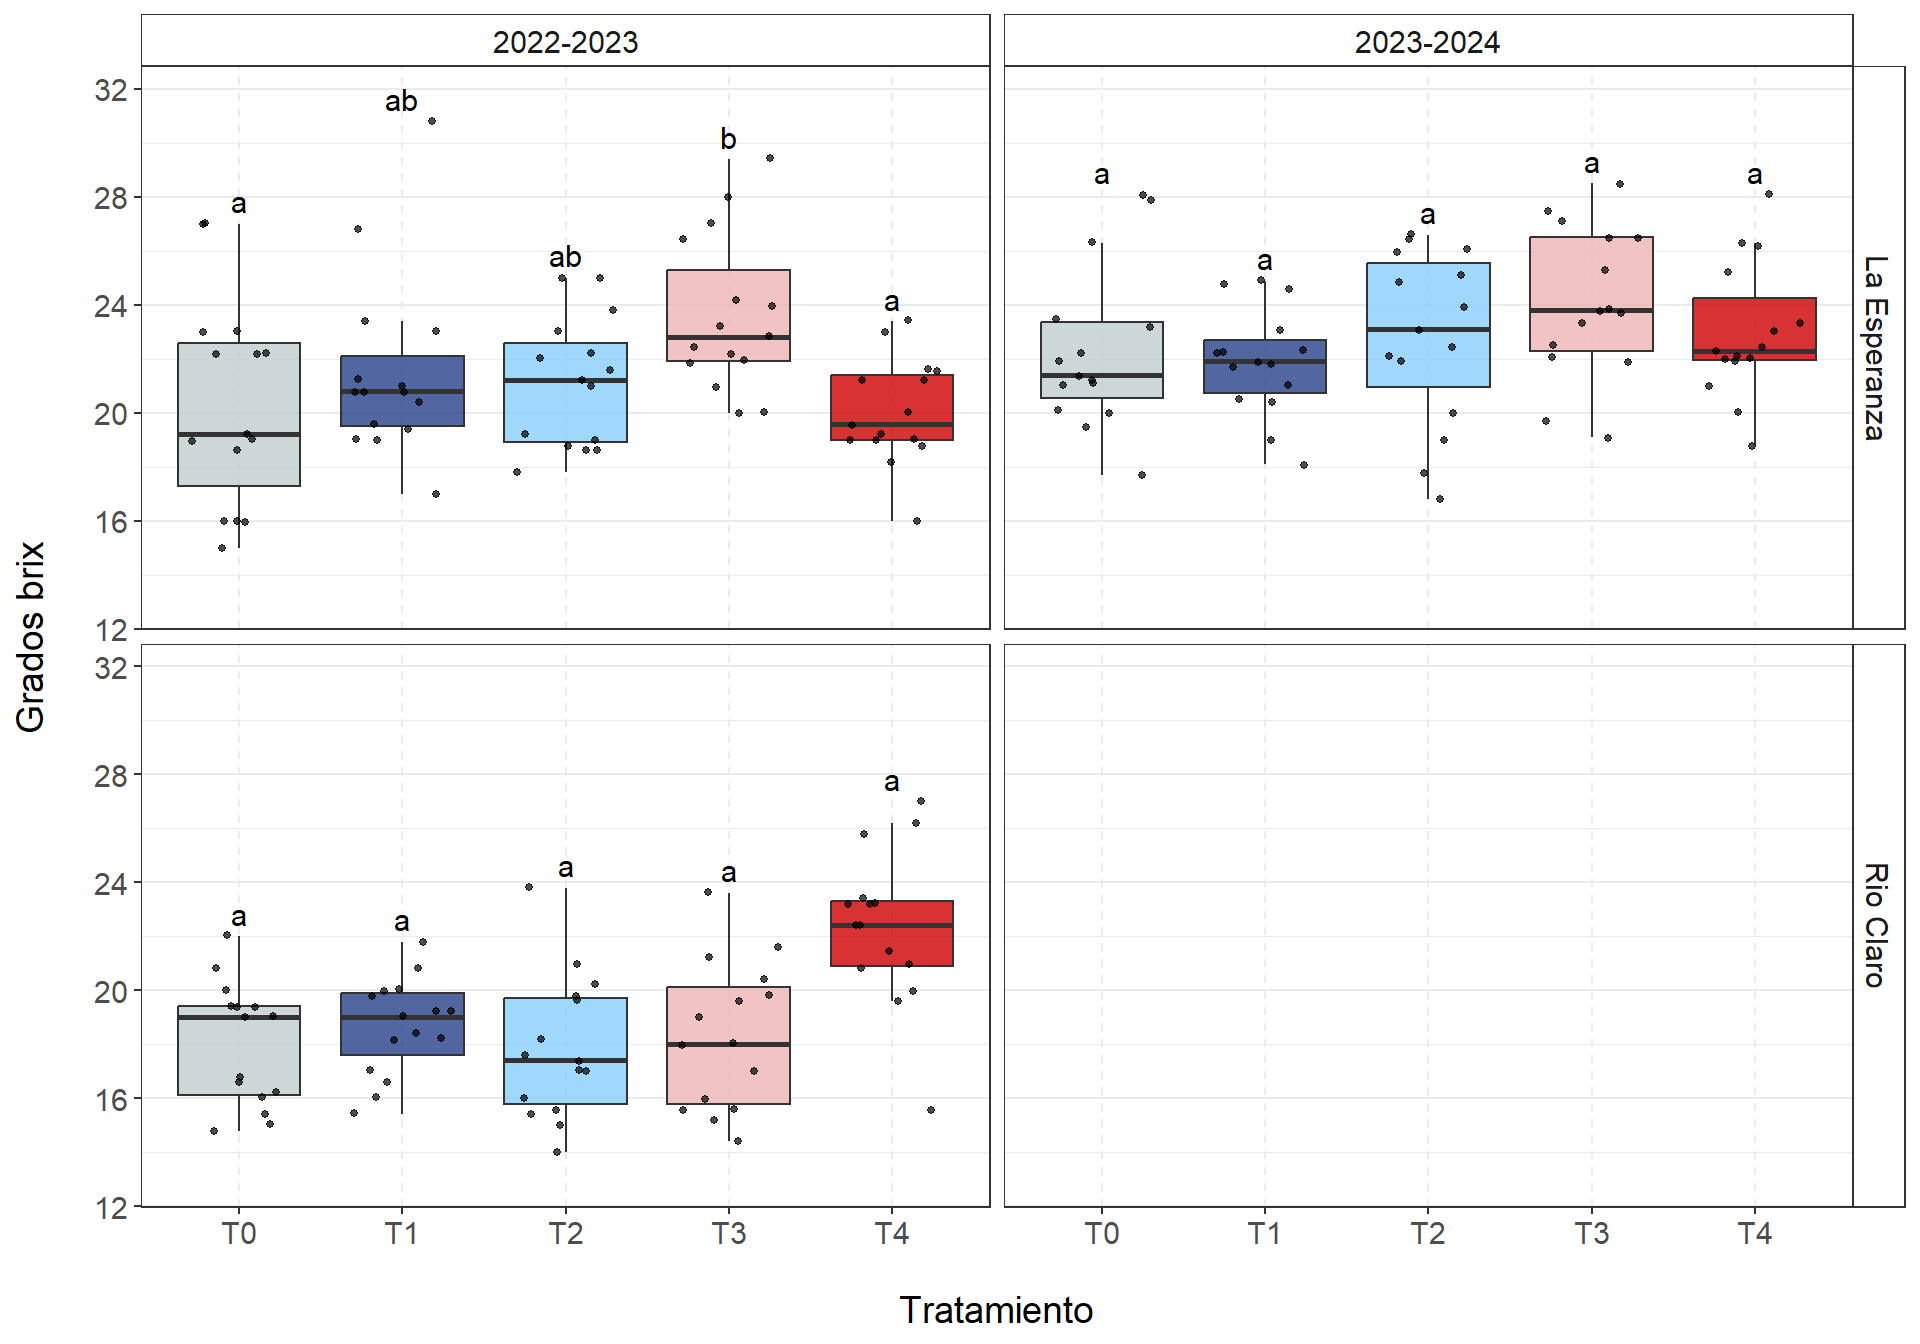
\includegraphics{0103_parametros_files/figure-pdf/unnamed-chunk-13-1.pdf}
\end{center}

\chapter{Serie temporal 2023-2024}

\begin{center}
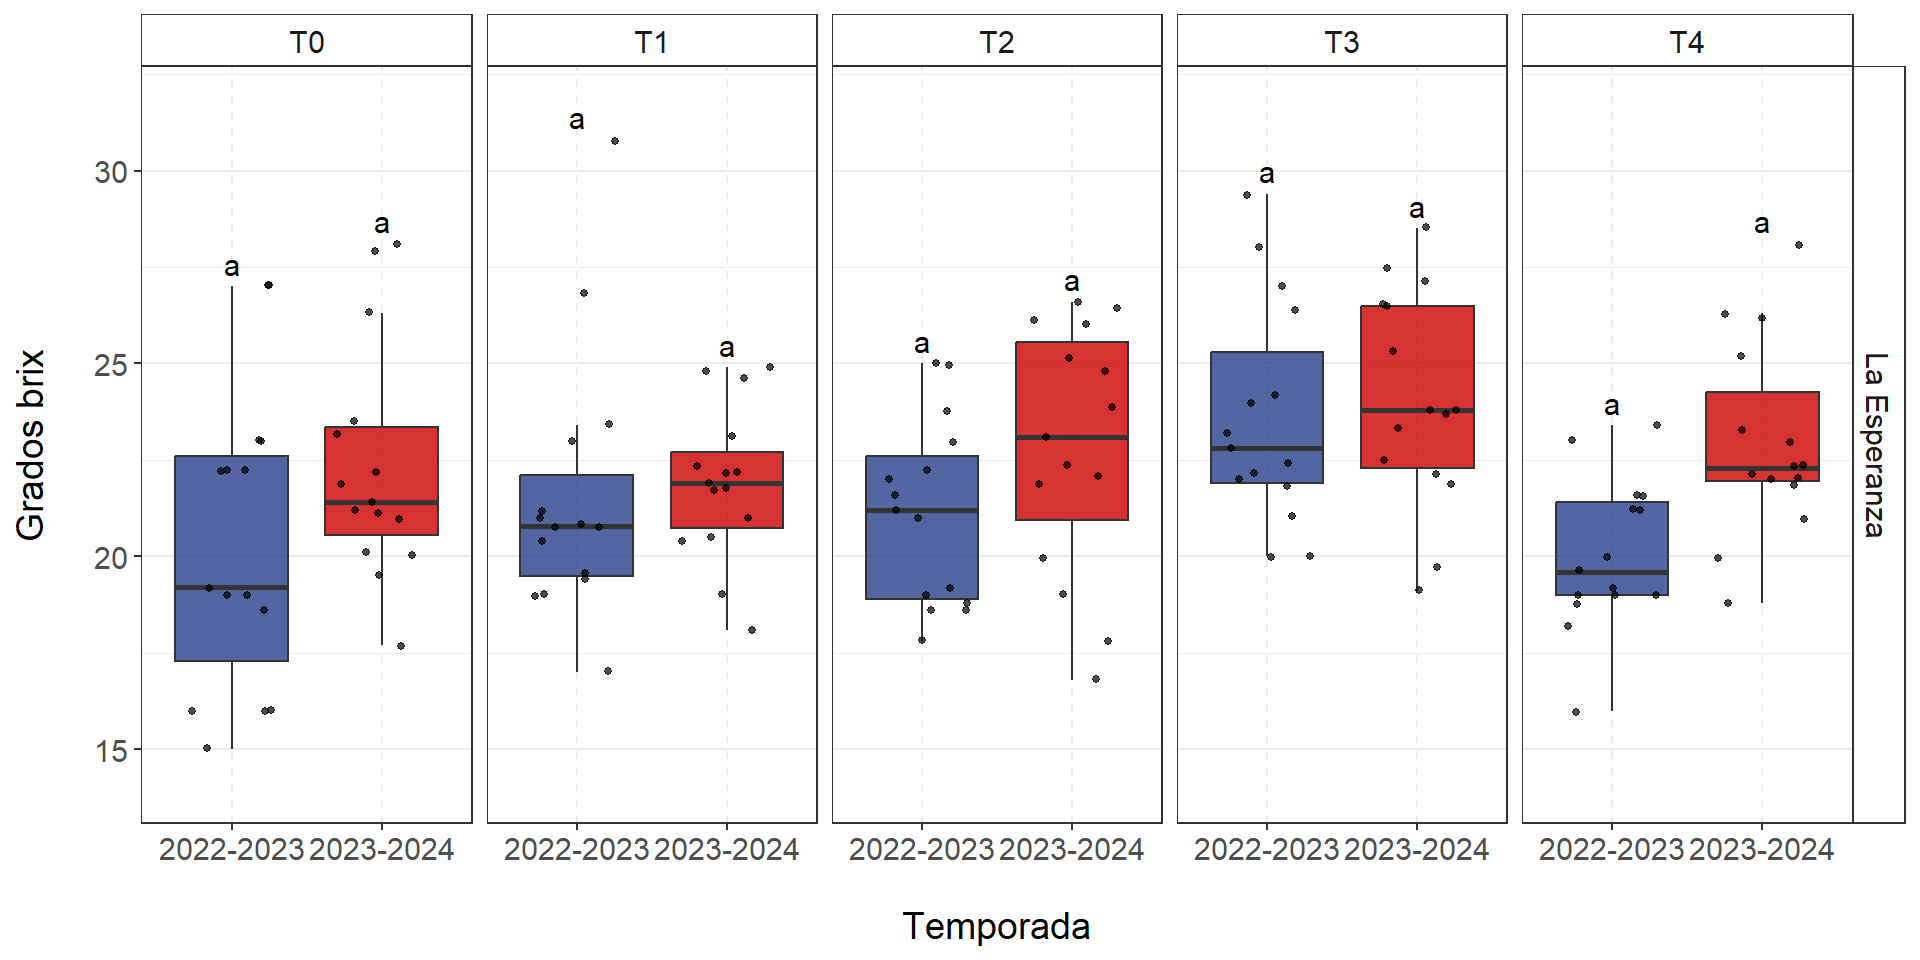
\includegraphics{0103_parametros_files/figure-pdf/unnamed-chunk-14-1.pdf}
\end{center}

\chapter{Ciclo diario 2022-2023}

\begin{center}
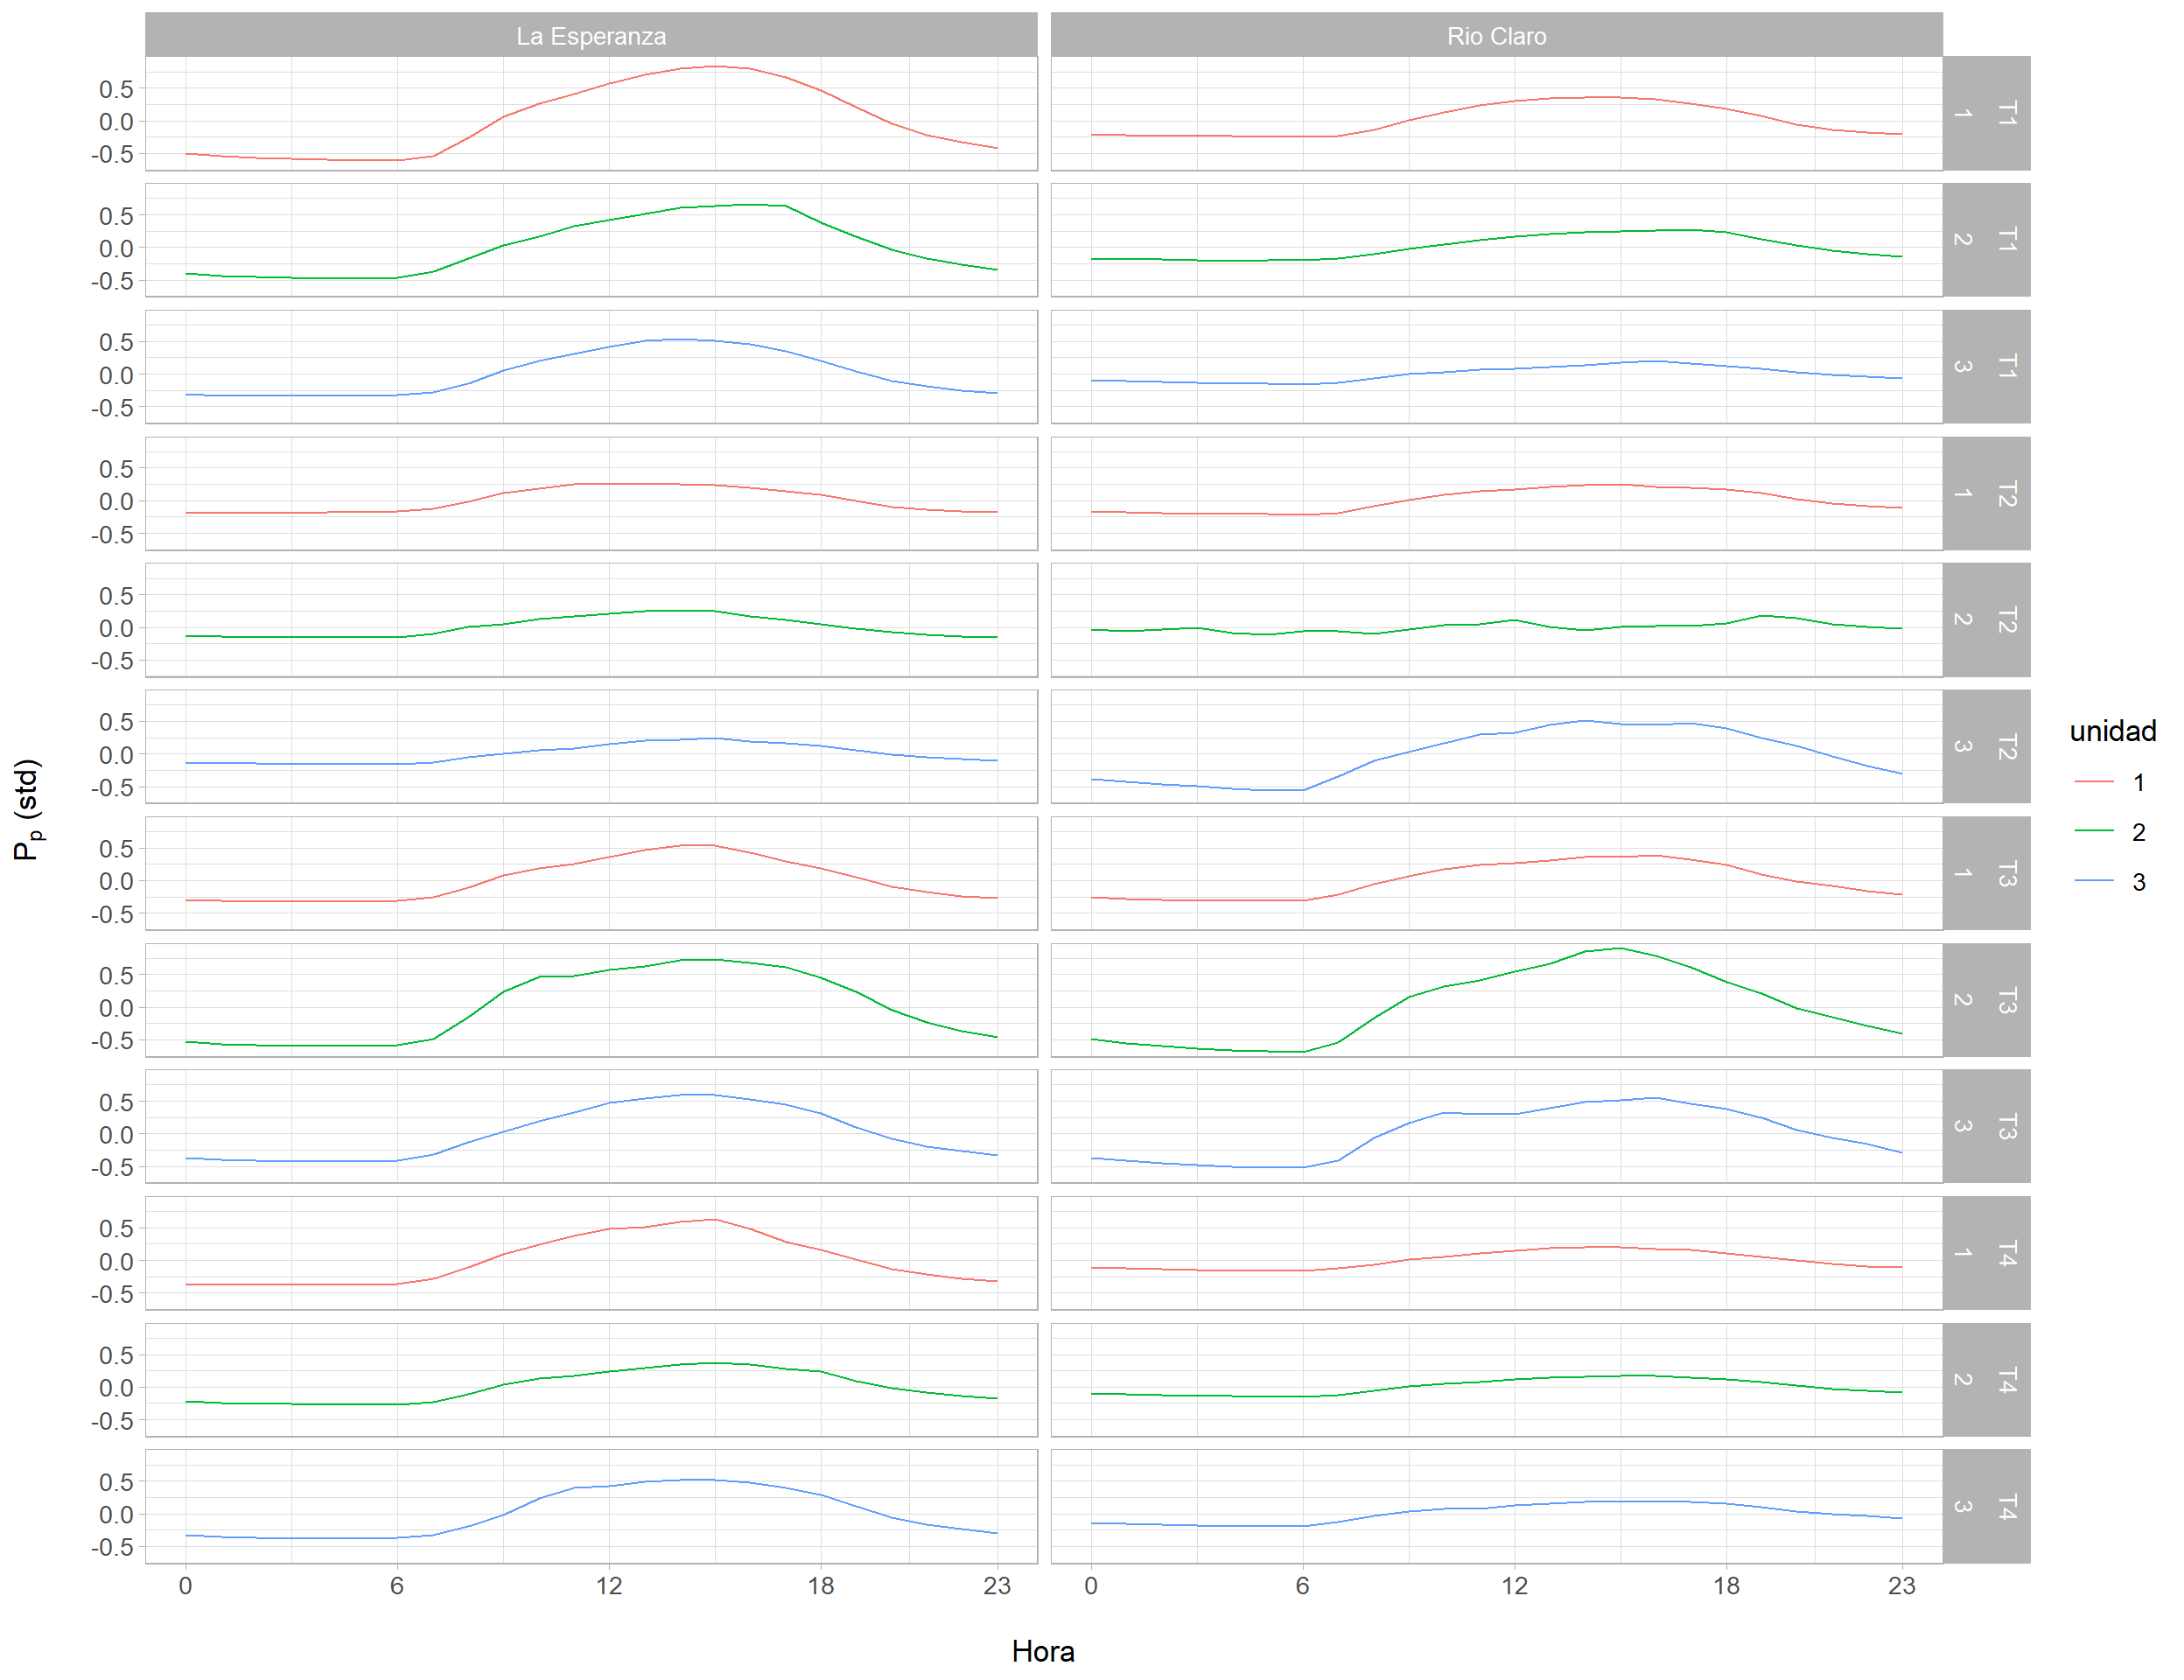
\includegraphics{0103_parametros_files/figure-pdf/unnamed-chunk-15-1.pdf}
\end{center}

\chapter{Ciclo diario 2023-2024}

\begin{center}
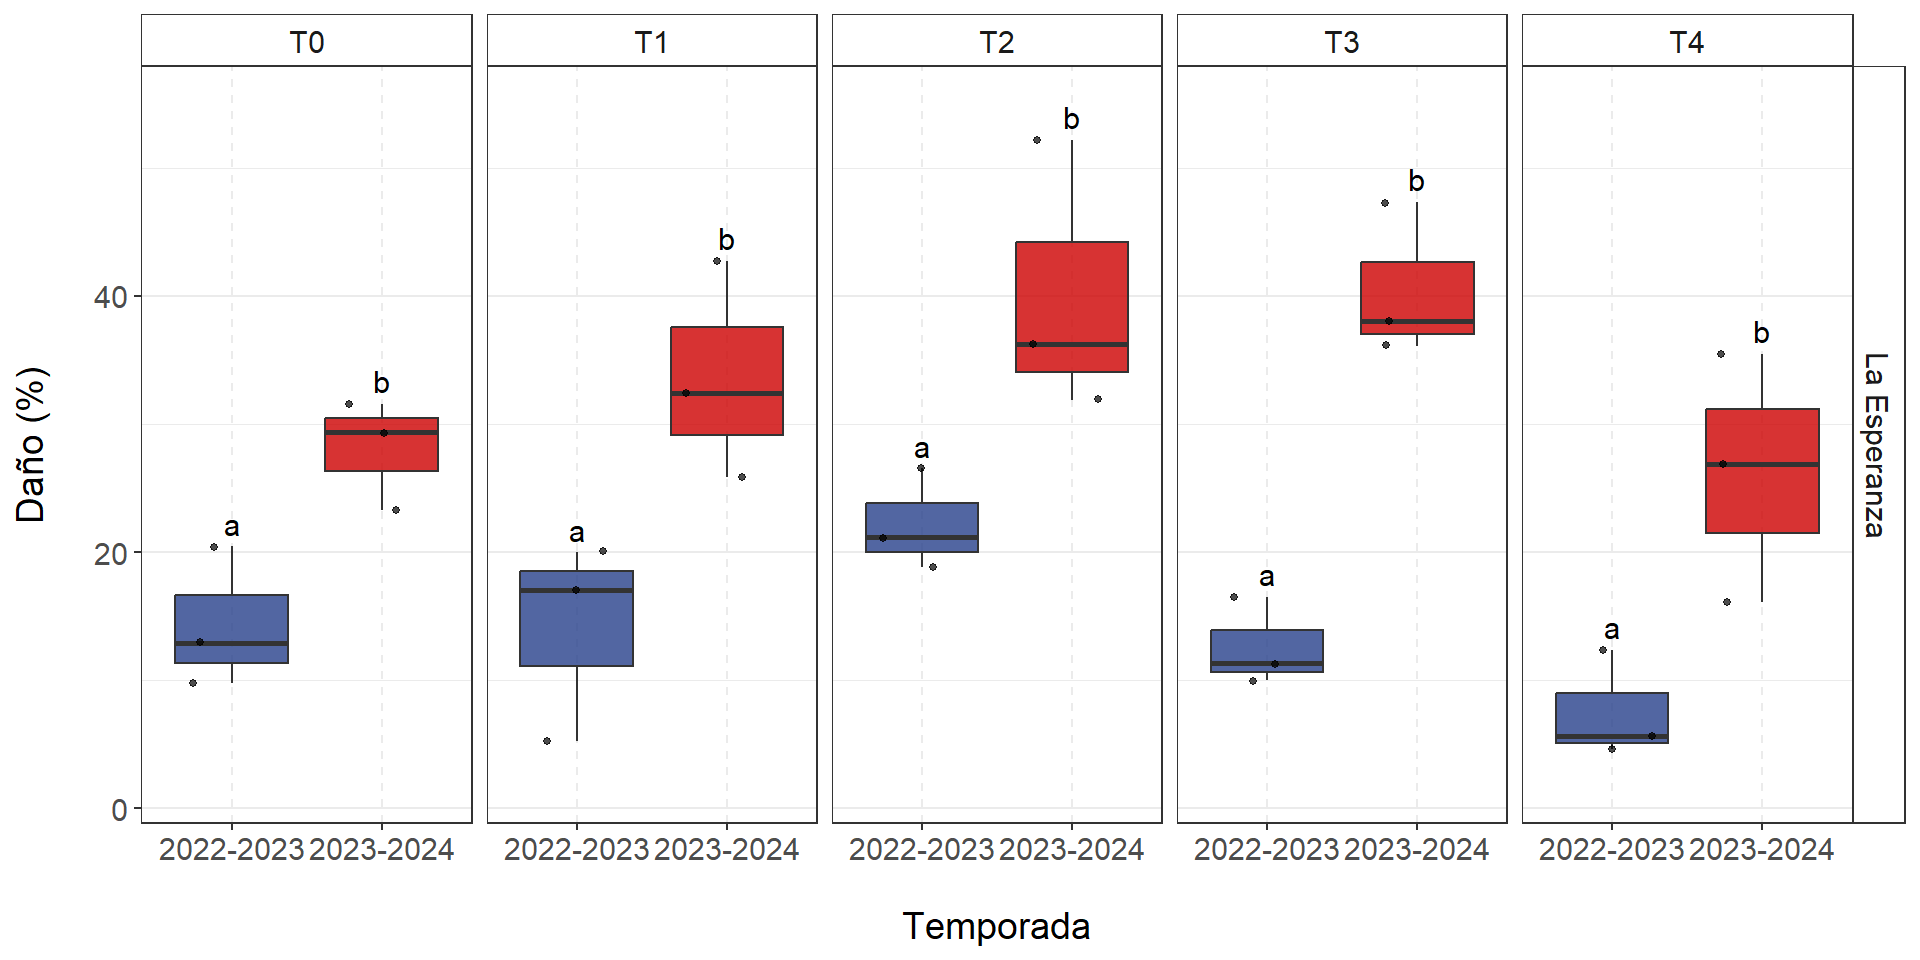
\includegraphics{0103_parametros_files/figure-pdf/unnamed-chunk-16-1.pdf}
\end{center}

\chapter{Población de datos}

La siguiente tabla presenta la población de datos según temporada, sitio
y tratamiento.

\begin{longtable}[]{@{}lllllr@{}}
\toprule\noalign{}
Temporada & Sitio & Tratamiento & Unidad & zim & n \\
\midrule\noalign{}
\endhead
\bottomrule\noalign{}
\endlastfoot
2022-2023 & La Esperanza & T1 & 1 & Z1 & 4749 \\
& & & & Z2 & 4418 \\
& & & 2 & Z1 & 4430 \\
& & & & Z2 & 4431 \\
& & & 3 & Z1 & 4417 \\
& & & & Z2 & 4417 \\
& & T2 & 1 & Z1 & 4028 \\
& & & & Z2 & 4028 \\
& & & 2 & Z1 & 3424 \\
& & & & Z2 & 3519 \\
& & & 3 & Z1 & 4102 \\
& & & & Z2 & 4408 \\
& & T3 & 1 & Z1 & 4124 \\
& & & & Z2 & 4124 \\
& & & 2 & Z1 & 4705 \\
& & & & Z2 & 4396 \\
& & & 3 & Z1 & 4374 \\
& & & & Z2 & 4726 \\
& & T4 & 1 & Z1 & 4418 \\
& & & & Z2 & 4102 \\
& & & 2 & Z1 & 4408 \\
& & & & Z2 & 4430 \\
& & & 3 & Z1 & 4417 \\
& & & & Z2 & 4410 \\
& Rio Claro & T1 & 1 & Z1 & 3964 \\
& & & & Z2 & 3941 \\
& & & 2 & Z1 & 3904 \\
& & & & Z2 & 3881 \\
& & & 3 & Z1 & 3857 \\
& & & & Z2 & 3879 \\
& & T2 & 1 & Z1 & 4088 \\
& & & & Z2 & 4089 \\
& & & 2 & Z1 & 1954 \\
& & & & Z2 & 1927 \\
& & & 3 & Z1 & 2702 \\
& & & & Z2 & 2927 \\
& & T3 & 1 & Z1 & 4295 \\
& & & & Z2 & 3942 \\
& & & 2 & Z1 & 4295 \\
& & & & Z2 & 4294 \\
& & & 3 & Z1 & 3263 \\
& & & & Z2 & 3592 \\
& & T4 & 1 & Z1 & 4256 \\
& & & & Z2 & 4255 \\
& & & 2 & Z1 & 3123 \\
& & & & Z2 & 3145 \\
& & & 3 & Z1 & 4175 \\
& & & & Z2 & 2883 \\
2023-2024 & La Esperanza & T1 & 1 & Z1 & 4300 \\
& & & & Z2 & 4300 \\
& & & 2 & Z1 & 4300 \\
& & & & Z2 & 4300 \\
& & & 3 & Z1 & 4299 \\
& & & & Z2 & 4299 \\
& & T2 & 1 & Z1 & 4296 \\
& & & & Z2 & 4296 \\
& & & 2 & Z1 & 3701 \\
& & & & Z2 & 3701 \\
& & & 3 & Z1 & 4297 \\
& & & & Z2 & 4297 \\
& & T3 & 1 & Z1 & 4292 \\
& & & & Z2 & 4292 \\
& & & 2 & Z1 & 4296 \\
& & & & Z2 & 4296 \\
& & & 3 & Z1 & 4295 \\
& & & & Z2 & 4295 \\
& & T4 & 1 & Z1 & 4301 \\
& & & & Z2 & 4301 \\
& & & 2 & Z1 & 4300 \\
& & & & Z2 & 4300 \\
& & & 3 & Z1 & 4300 \\
& & & & Z2 & 4299 \\
& Rio Claro & T1 & 1 & Z1 & 3842 \\
& & & & Z2 & 3841 \\
& & & 2 & Z1 & 1678 \\
& & & & Z2 & 1678 \\
& & & 3 & Z1 & 3842 \\
& & & & Z2 & 3842 \\
& & T2 & 1 & Z1 & 3619 \\
& & & & Z2 & 3619 \\
& & & 2 & Z1 & 3943 \\
& & & & Z2 & 3943 \\
& & & 3 & Z1 & 3538 \\
& & & & Z2 & 3538 \\
& & T3 & 1 & Z1 & 3843 \\
& & & & Z2 & 3841 \\
& & & 2 & Z1 & 3842 \\
& & & & Z2 & 3840 \\
& & & 3 & Z1 & 3843 \\
& & & & Z2 & 3841 \\
& & T4 & 1 & Z1 & 3842 \\
& & & & Z2 & 3842 \\
& & & 2 & Z1 & 3536 \\
& & & & Z2 & 3536 \\
& & & 3 & Z1 & 3843 \\
& & & & Z2 & 3843 \\
\end{longtable}

\chapter{Humedad de suelo}\label{humedad-de-suelo}

Los datos de humedad de suelo se recopilaron mediante sensores ubicados
en cada unidad de medición. Estos se conectaron al transmisor Yara igual
que los sensores ZIM de turgor, y proporcionaron datos contínuos de
humedad de suelo (\%VWC) cada media hora para los dos sitios durante
ambas temporadas.

\chapter{Distribución}

\begin{center}
\includegraphics{0104_humedad_files/figure-pdf/unnamed-chunk-2-1.pdf}
\end{center}

\chapter{Serie temporal 2022-2023}

\begin{center}
\includegraphics{0104_humedad_files/figure-pdf/unnamed-chunk-3-1.pdf}
\end{center}

\chapter{Serie temporal 2023-2024}

\begin{center}
\includegraphics{0104_humedad_files/figure-pdf/unnamed-chunk-4-1.pdf}
\end{center}

\chapter{Población de datos}

La siguiente tabla presenta la población de datos según temporada, sitio
y tratamiento.

\begin{longtable}[]{@{}llllr@{}}
\toprule\noalign{}
Temporada & Sitio & Tratamiento & Unidad & n \\
\midrule\noalign{}
\endhead
\bottomrule\noalign{}
\endlastfoot
2022-2023 & La Esperanza & T1 & 1 & 3013 \\
& & & 2 & 3013 \\
& & & 3 & 3013 \\
& & T2 & 1 & 2610 \\
& & & 2 & 1510 \\
& & & 3 & 3013 \\
& & T3 & 1 & 3013 \\
& & & 2 & 3013 \\
& & & 3 & 3013 \\
& & T4 & 1 & 3013 \\
& & & 2 & 3013 \\
& & & 3 & 3013 \\
& Rio Claro & T1 & 1 & 3013 \\
& & & 2 & 3000 \\
& & & 3 & 2940 \\
& & T2 & 1 & 1639 \\
& & & 2 & 1141 \\
& & & 3 & 2415 \\
& & T3 & 1 & 3013 \\
& & & 2 & 3013 \\
& & & 3 & 3013 \\
& & T4 & 1 & 3005 \\
& & & 2 & 1801 \\
& & & 3 & 3010 \\
2023-2024 & La Esperanza & T1 & 1 & 829 \\
& & & 2 & 3743 \\
& & & 3 & 3741 \\
& & T2 & 1 & 3737 \\
& & & 3 & 2689 \\
& & T3 & 1 & 3738 \\
& & & 2 & 3742 \\
& & & 3 & 3741 \\
& & & 2 & 831 \\
& & & 3 & 3740 \\
& Rio Claro & T1 & 1 & 807 \\
& & & 2 & 1962 \\
& & & 3 & 4165 \\
& & T2 & 1 & 3939 \\
& & & 2 & 3725 \\
& & & 3 & 3825 \\
& & T3 & 1 & 4162 \\
& & & 2 & 4163 \\
& & & 3 & 4165 \\
& & T4 & 1 & 4126 \\
& & & 2 & 722 \\
& & & 3 & 236 \\
\end{longtable}

\chapter{Clima}\label{clima}

Las variables climáticas fueron obtenidas de las estaciones
meteorológicas de Garces Fruits ubicadas en ambos sitios.

\chapter{Temperatura}

\begin{center}
\includegraphics{0105_clima_files/figure-pdf/unnamed-chunk-3-1.pdf}
\end{center}

\chapter{Déficit de presión de vapor (VPD)}

\begin{center}
\includegraphics{0105_clima_files/figure-pdf/unnamed-chunk-4-1.pdf}
\end{center}

\chapter{Evapotranspiración de referencia (ET0)}

\begin{center}
\includegraphics{0105_clima_files/figure-pdf/unnamed-chunk-5-1.pdf}
\end{center}

\chapter{Precipitación}

\begin{center}
\includegraphics{0105_clima_files/figure-pdf/unnamed-chunk-6-1.pdf}
\end{center}

\chapter{Curva Presión-volumen}\label{sec-pv}

Los datos utilizados para las curvas Presión-volumen corresponden a
mediciones de potencial hídrico xilemático y peso en hojas tomadas en
laboratorio con cámara de presión Scholander y balanza analítica.
{[}Metodología de toma de datos{]}.

Según la metodología descrita por Halbritter et~al. (2020), el punto de
pérdida de turgor (TLP) se estima como el último punto de la curva del Ψ
inverso en función del RWD (1 - RWC) antes de comenzar su fracción
lineal, como se muestra en la Figura~\ref{fig-tlp}.

\begin{figure}

\centering{

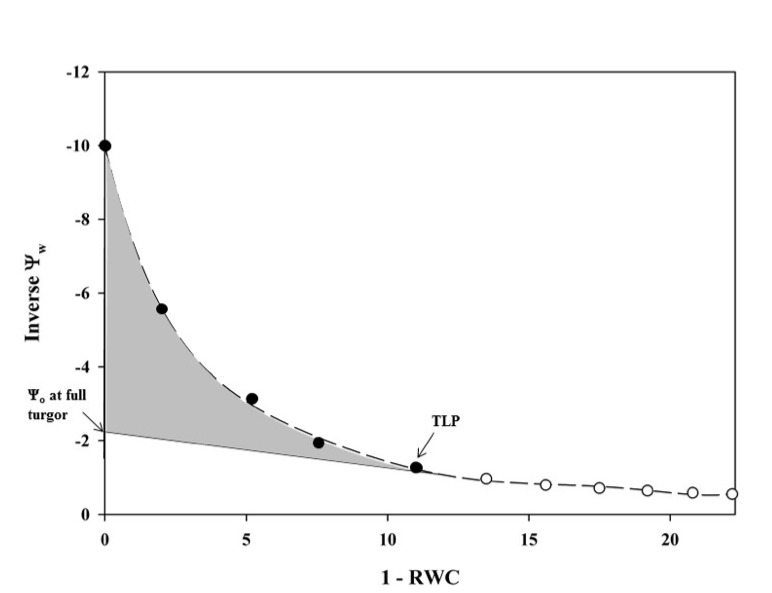
\includegraphics{figuras/misc/tlp.png}

}

\caption{\label{fig-tlp}Ejemplo de una curva presión-volumen. Los
círculos llenos representan las primeras 5 mediciones iterativas: los
círculos abiertos representan las últimas 6 mediciones. La porción
lineal (línea sólida) muestra el potencial osmótico (Ψo), la porción
curva (línea discontinua) es el potencial hídrico antes del punto de
pérdida de turgencia (TLP), y el área sombreada es el potencial de
turgencia (Ψp).Fuente: Halbritter et~al. (2020) (2020).}

\end{figure}%

En base a esta misma metodología, a continuación se presentan las curvas
presión-volumen de cada unidad medida.

\section{La Esperanza}\label{la-esperanza}

\chapter{Tratamiento 0 (control)}

Unidad 1 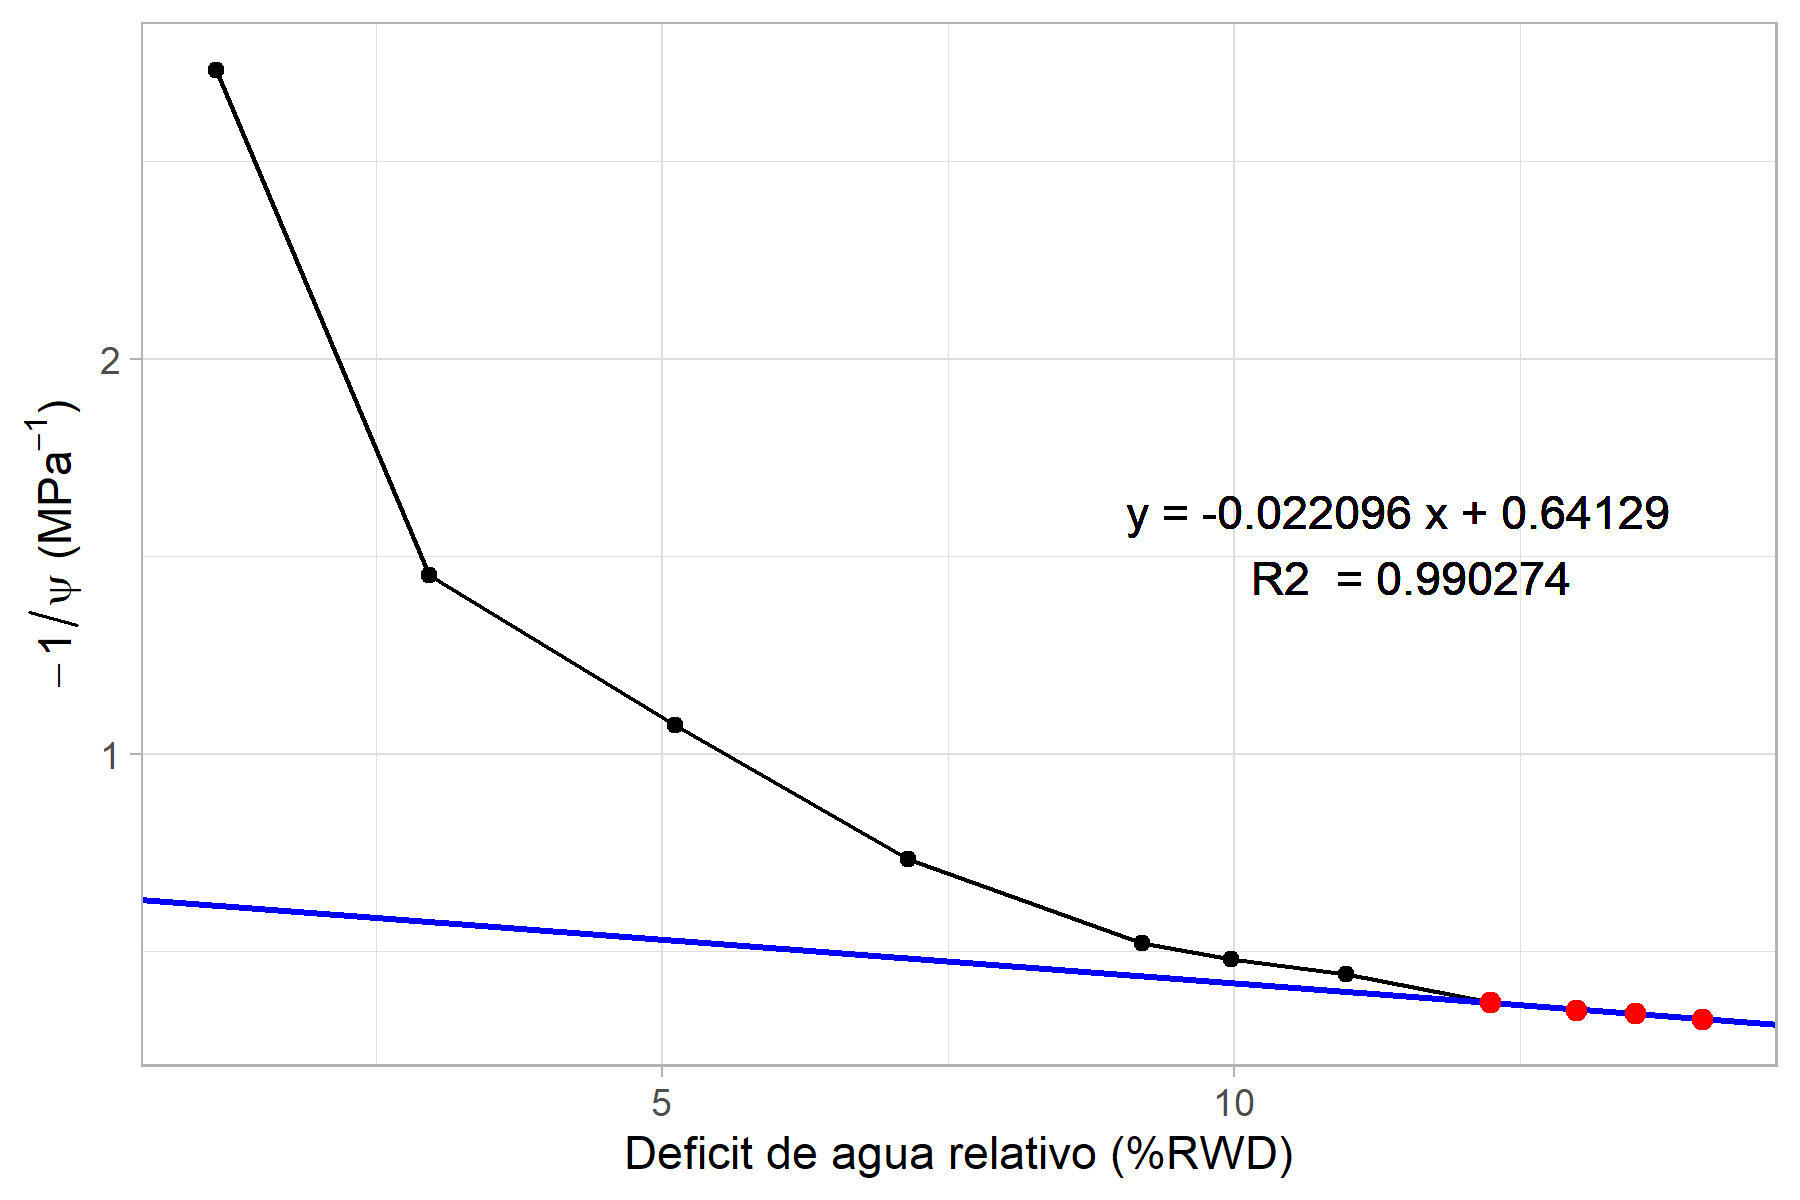
\includegraphics{figuras/06_tlp/tlp_la_esperanza_T0_1.png}

Unidad 2 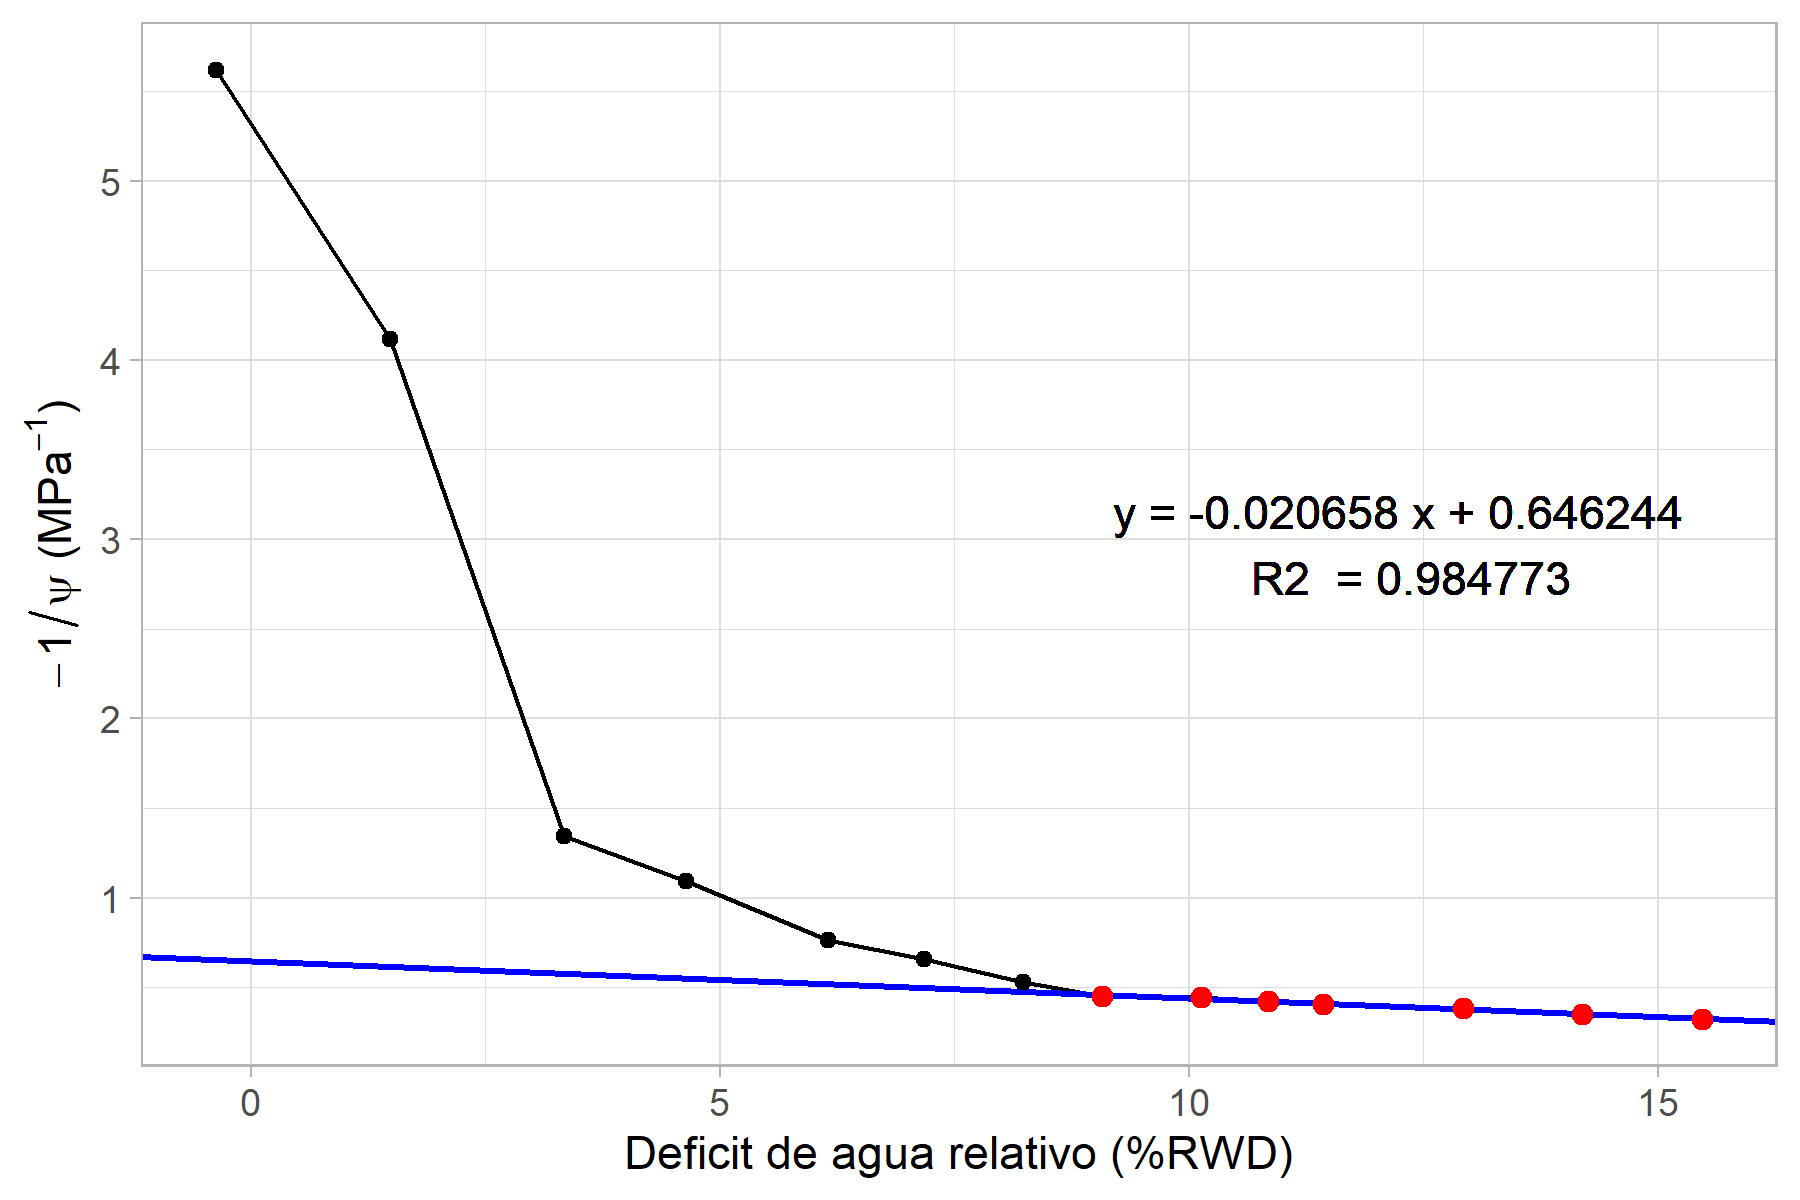
\includegraphics{figuras/06_tlp/tlp_la_esperanza_T0_2.png}

Unidad 3 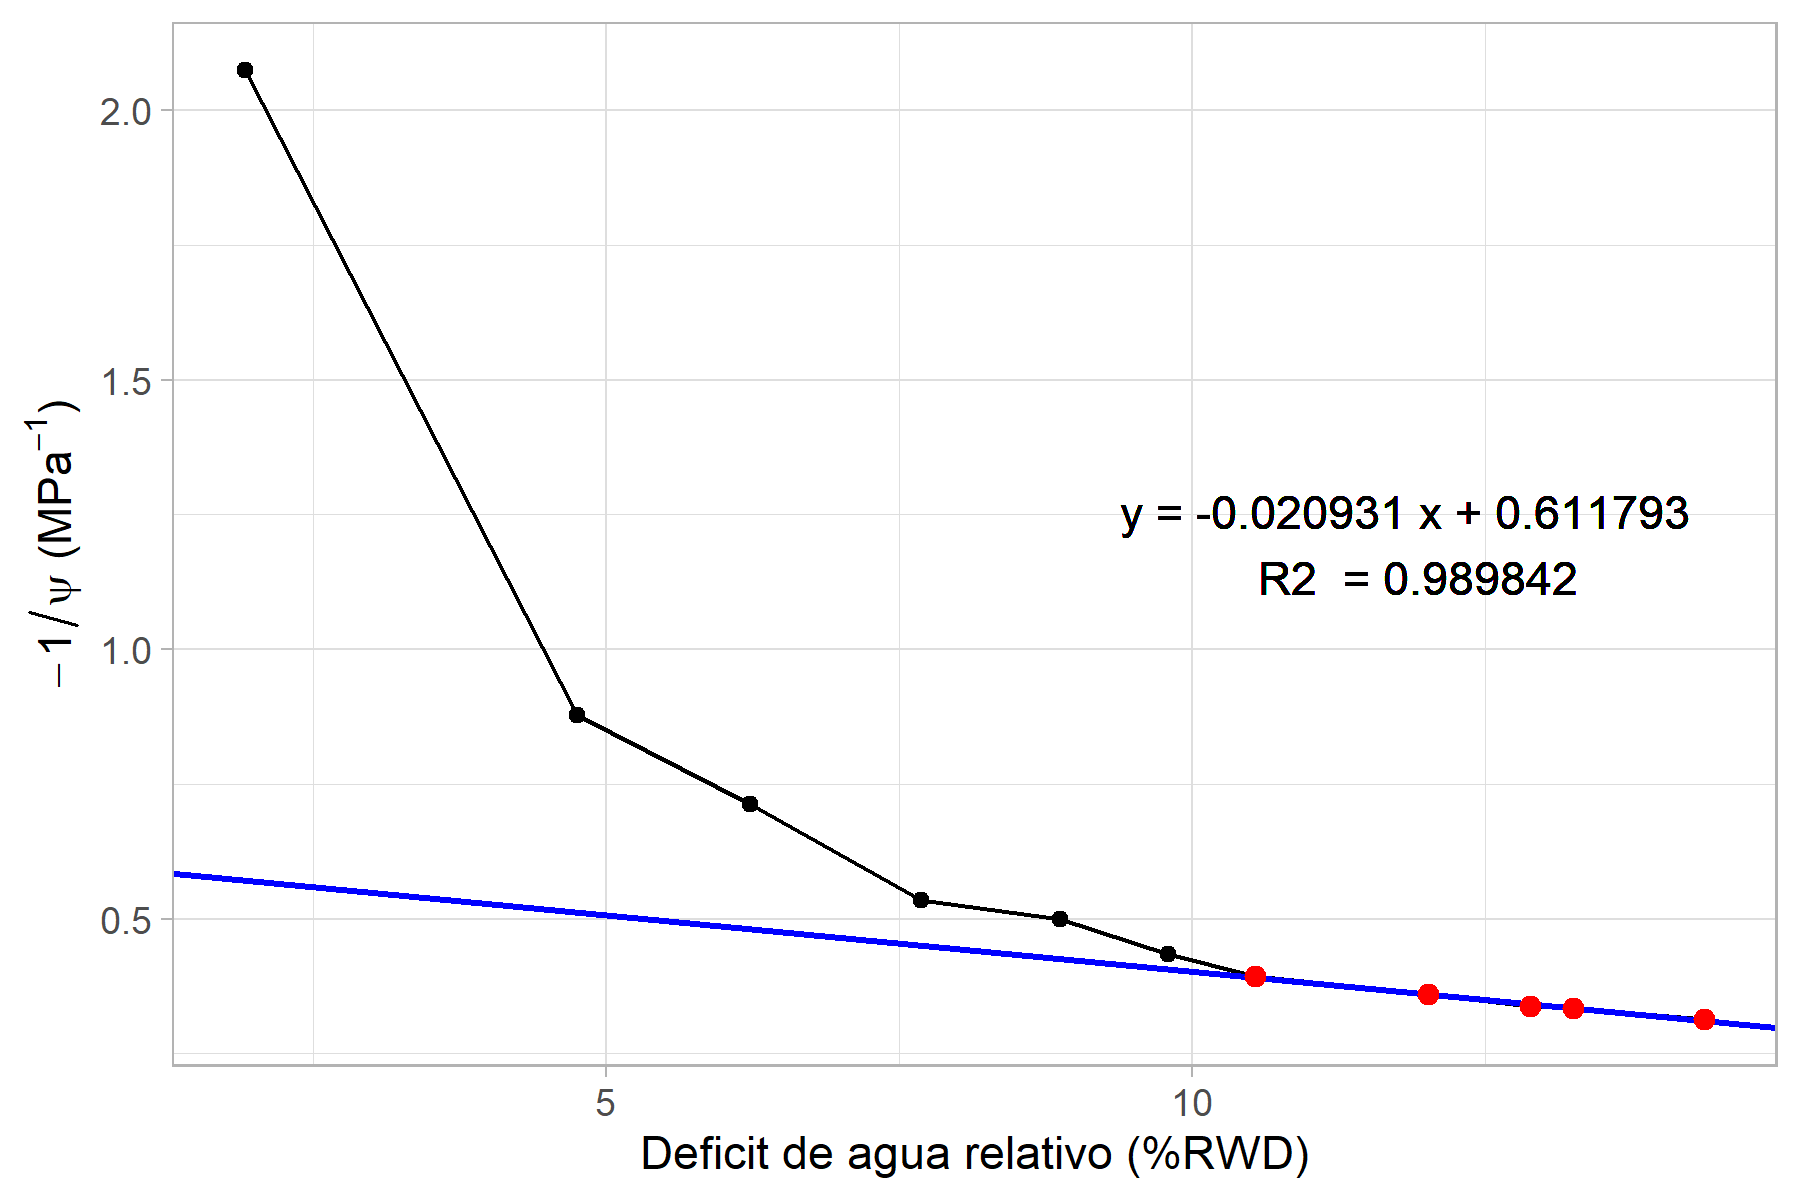
\includegraphics{figuras/06_tlp/tlp_la_esperanza_T0_3.png}

\chapter{Tratamiento 4}

Unidad 1 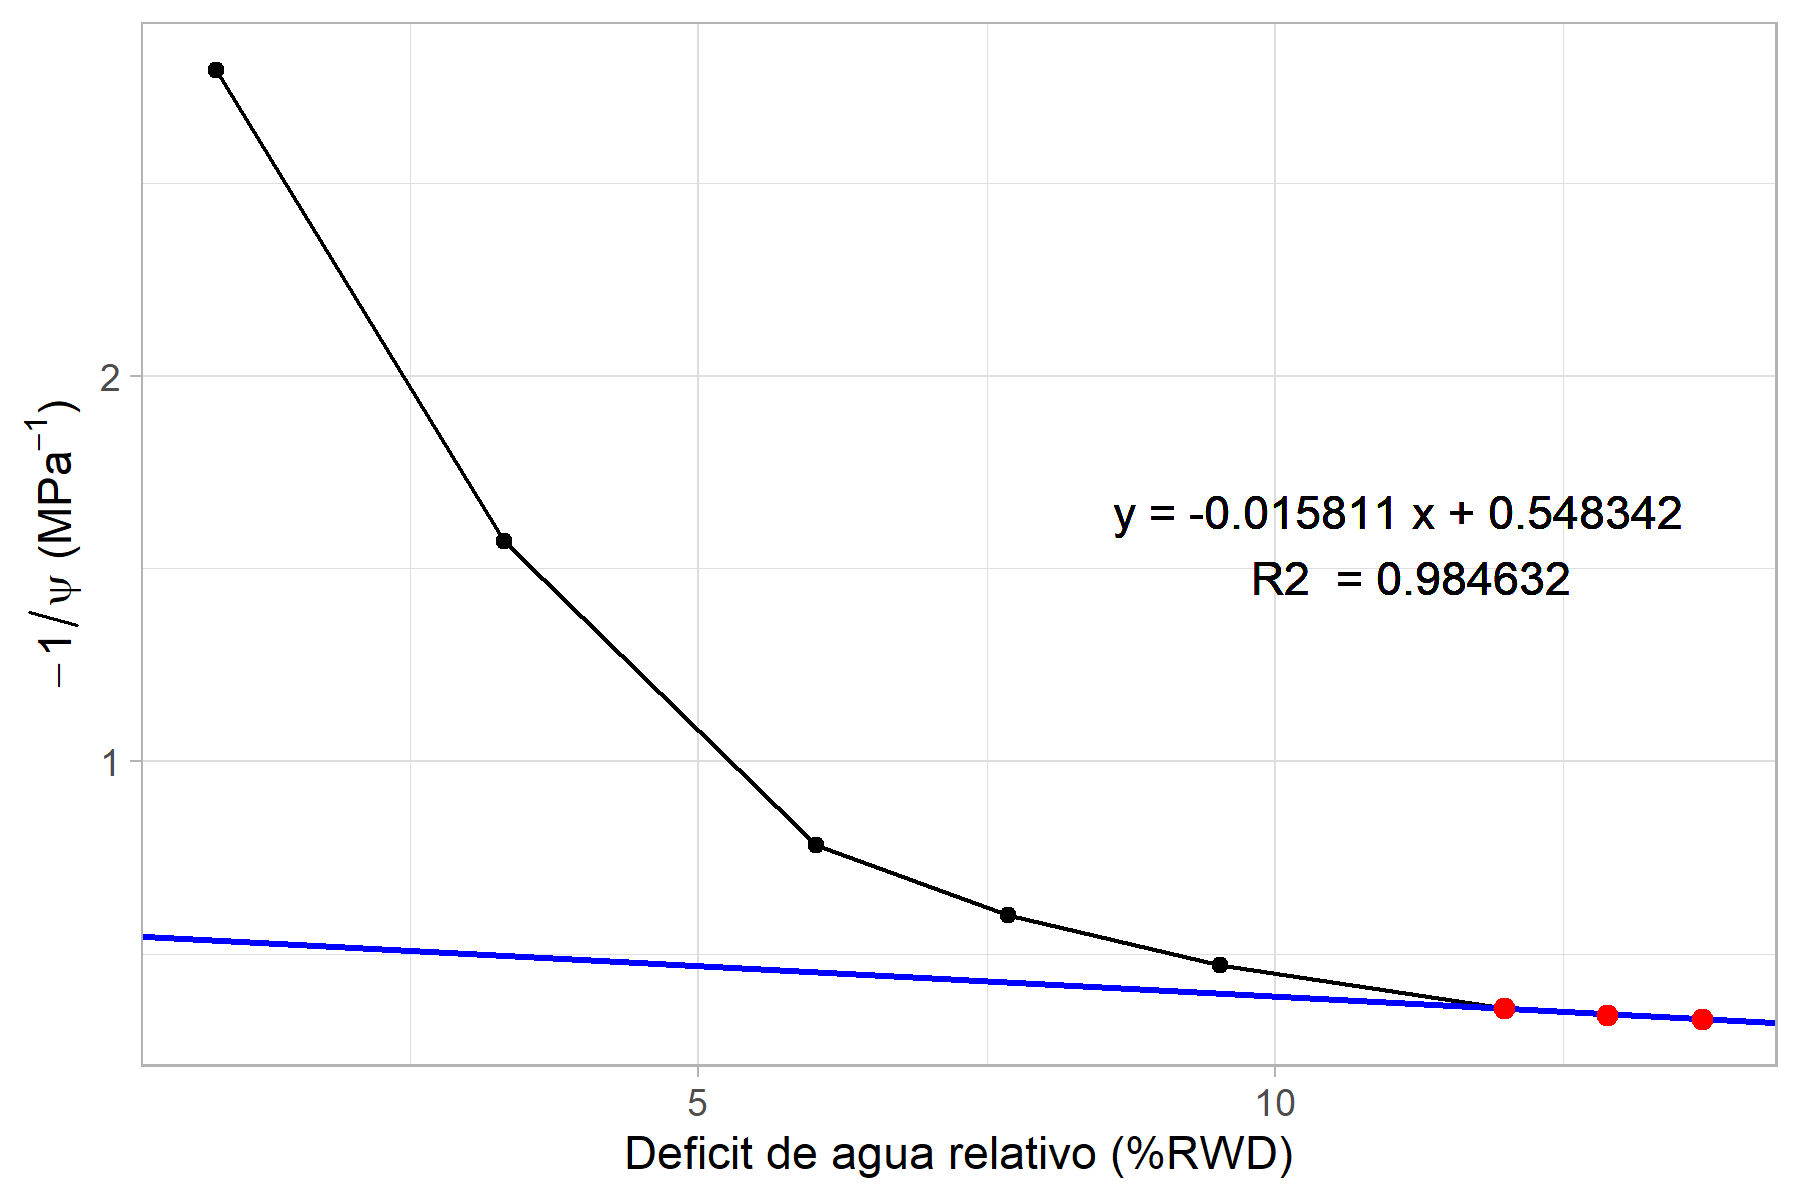
\includegraphics{figuras/06_tlp/tlp_la_esperanza_T4_1.png}

Unidad 2 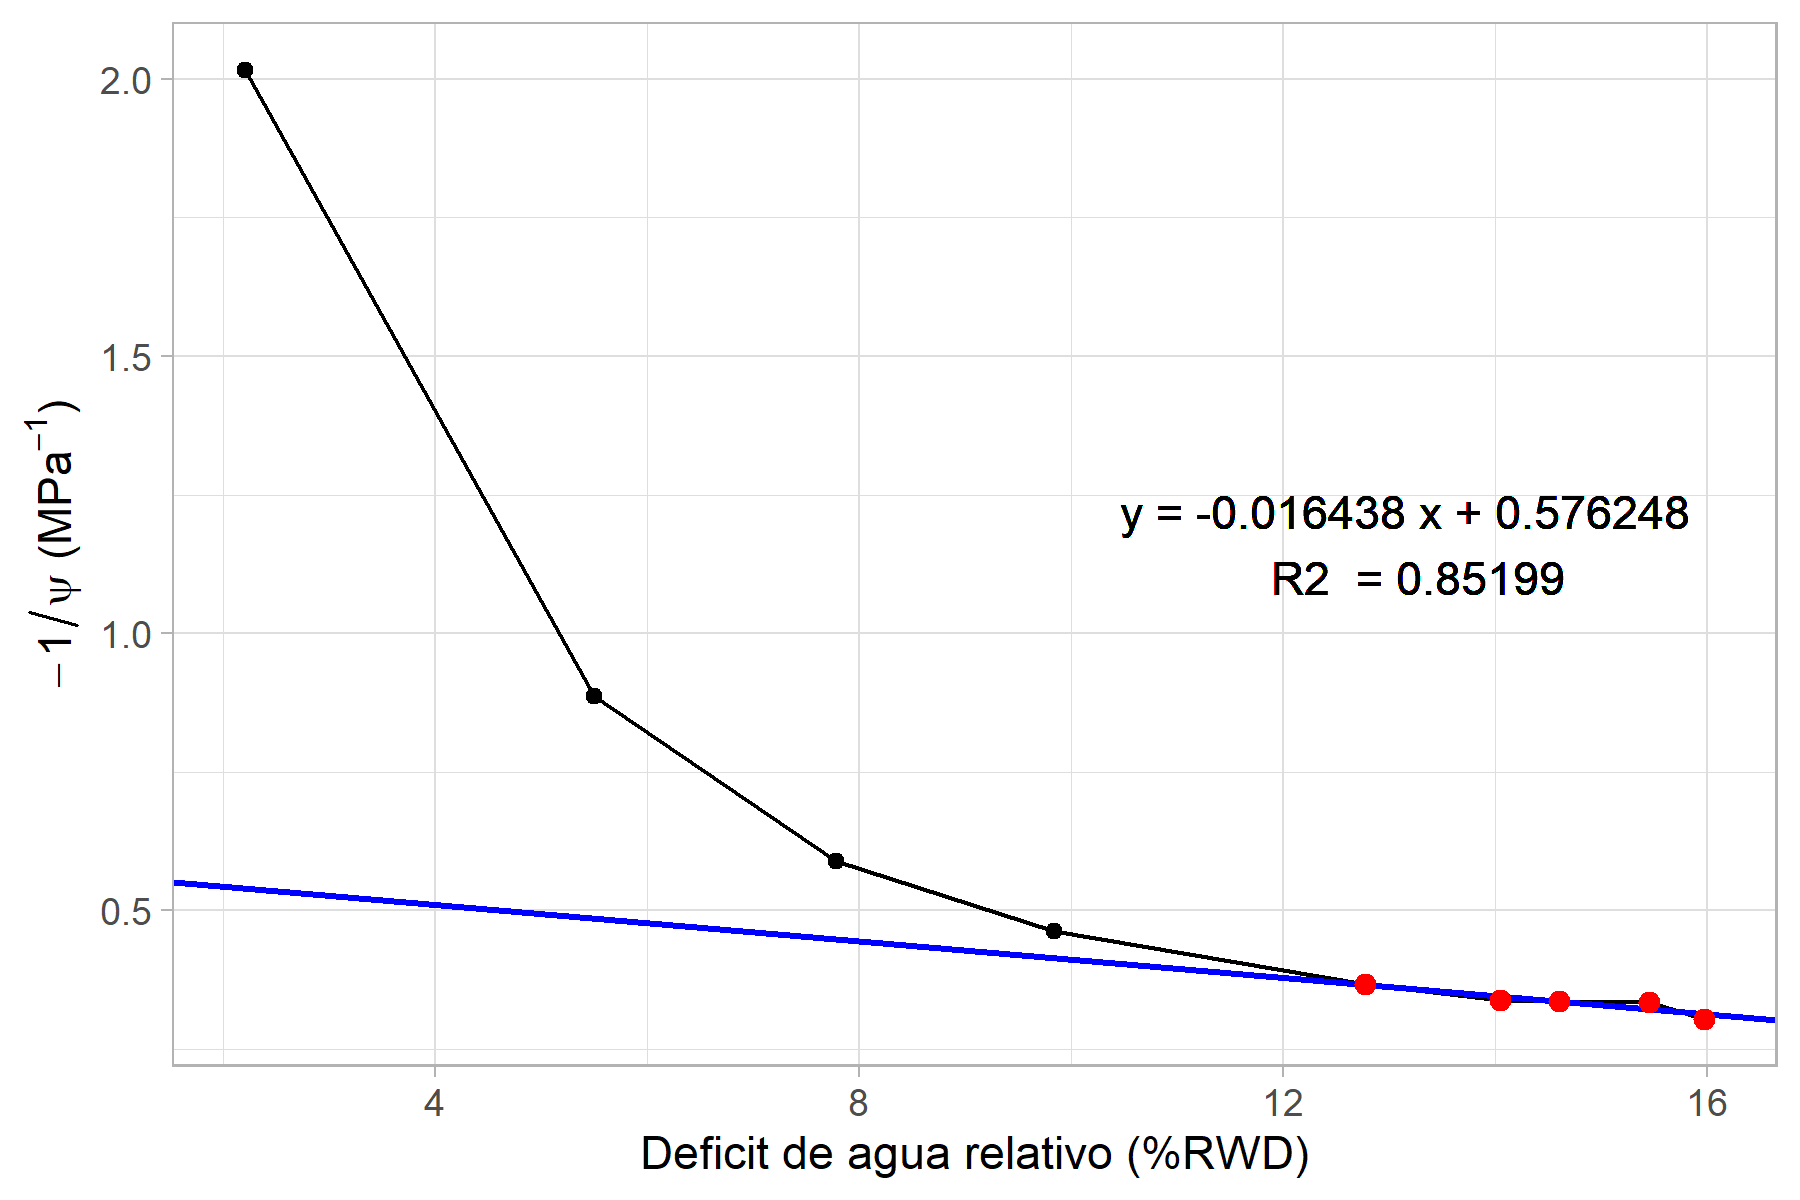
\includegraphics{figuras/06_tlp/tlp_la_esperanza_T4_2.png}

Unidad 3 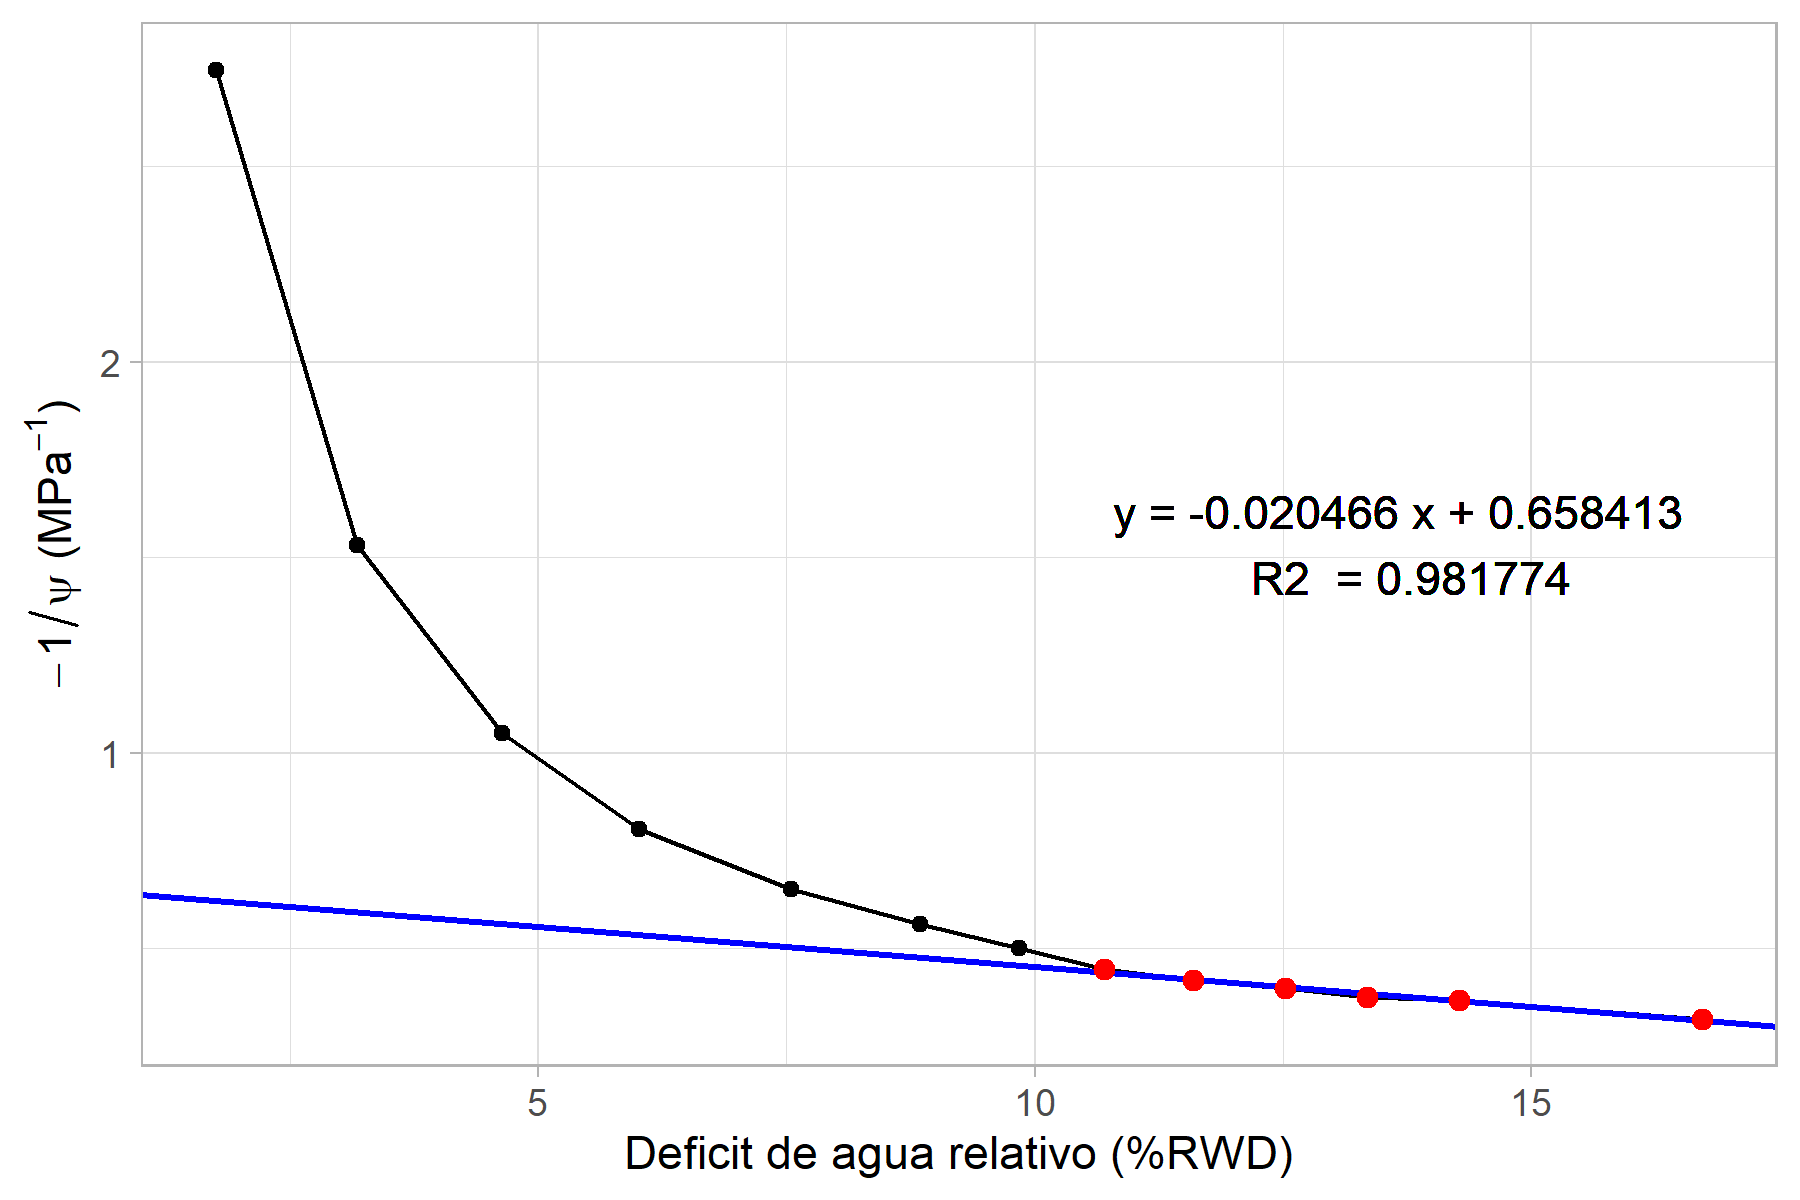
\includegraphics{figuras/06_tlp/tlp_la_esperanza_T4_3.png}

\section{Rio Claro}\label{rio-claro}

\chapter{Tratamiento 0 (control)}

Unidad 1 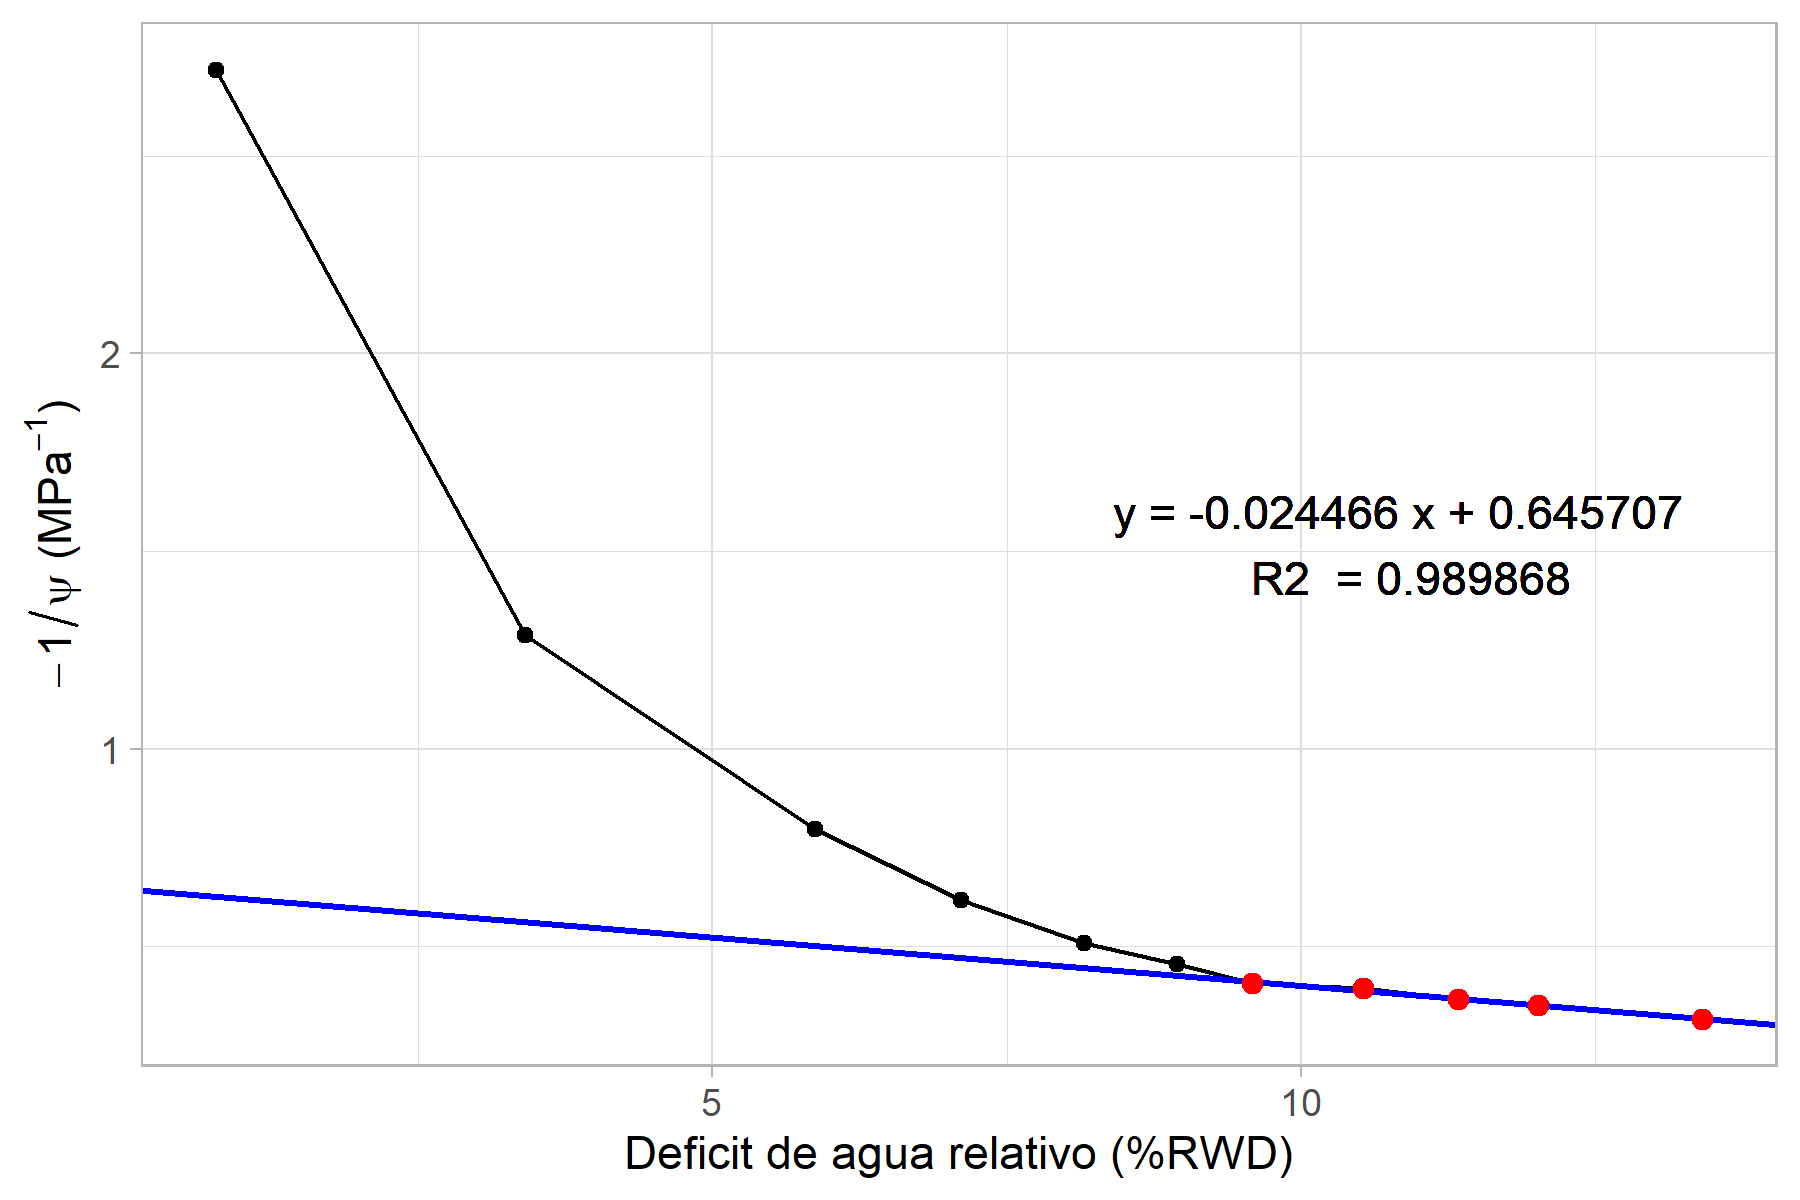
\includegraphics{figuras/06_tlp/tlp_rio_claro_T0_1.png}

Unidad 2 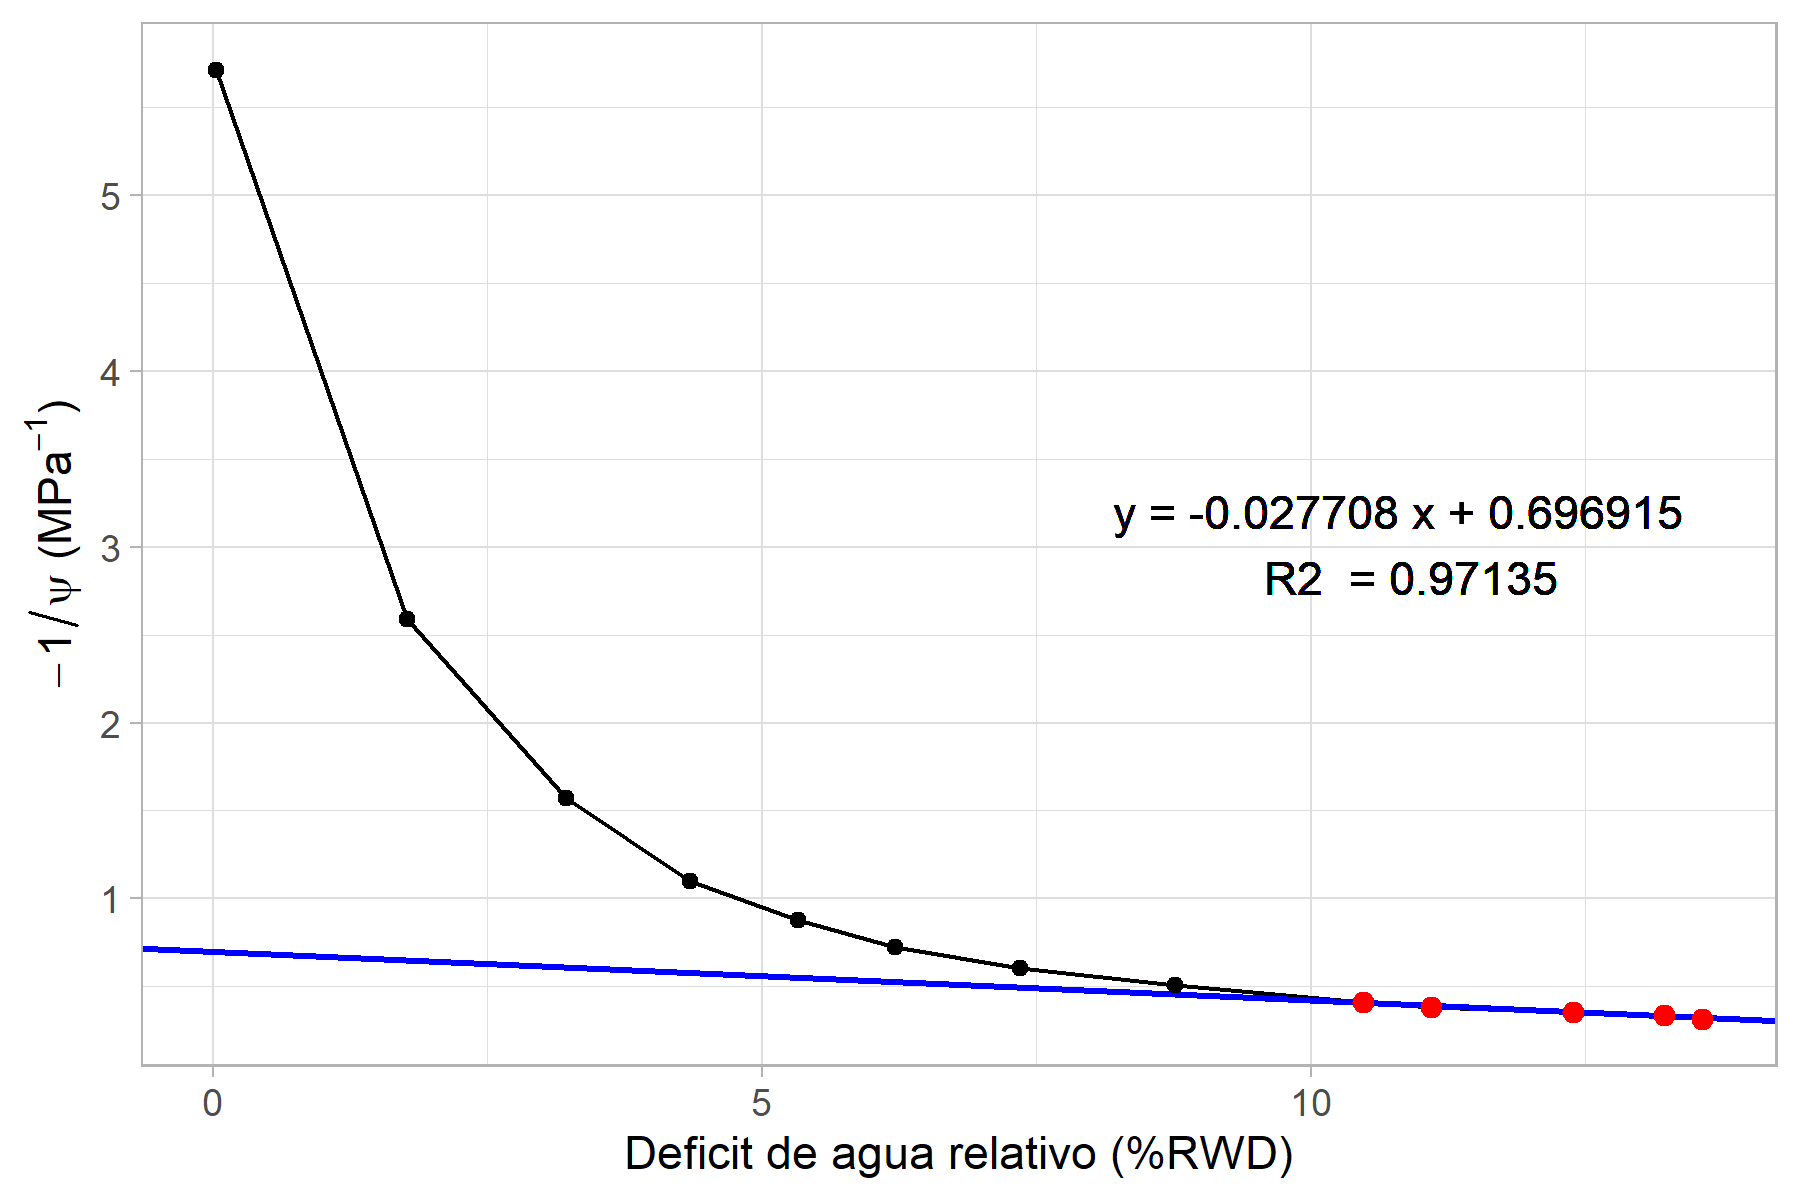
\includegraphics{figuras/06_tlp/tlp_rio_claro_T0_2.png}

Unidad 3 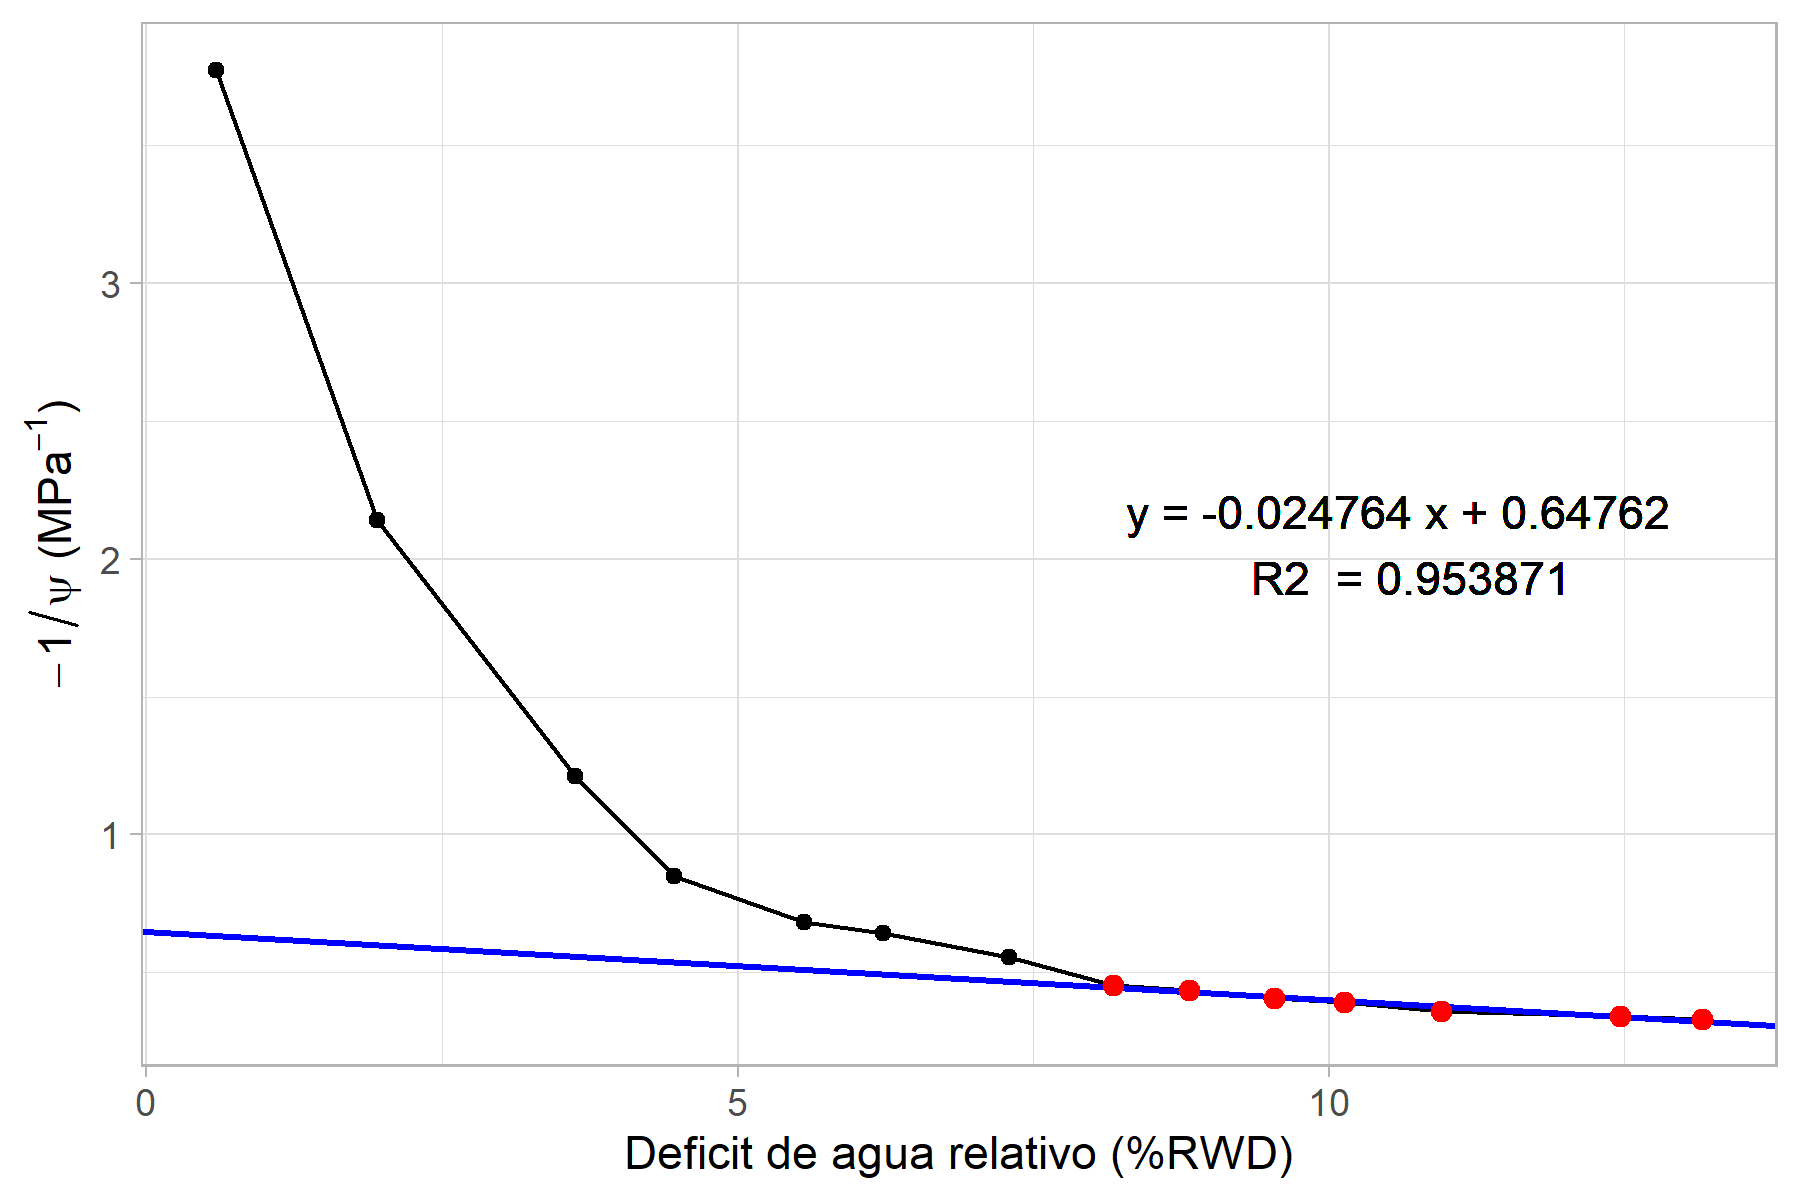
\includegraphics{figuras/06_tlp/tlp_rio_claro_T0_3.png}

\chapter{Tratamiento 1}

Unidad 1 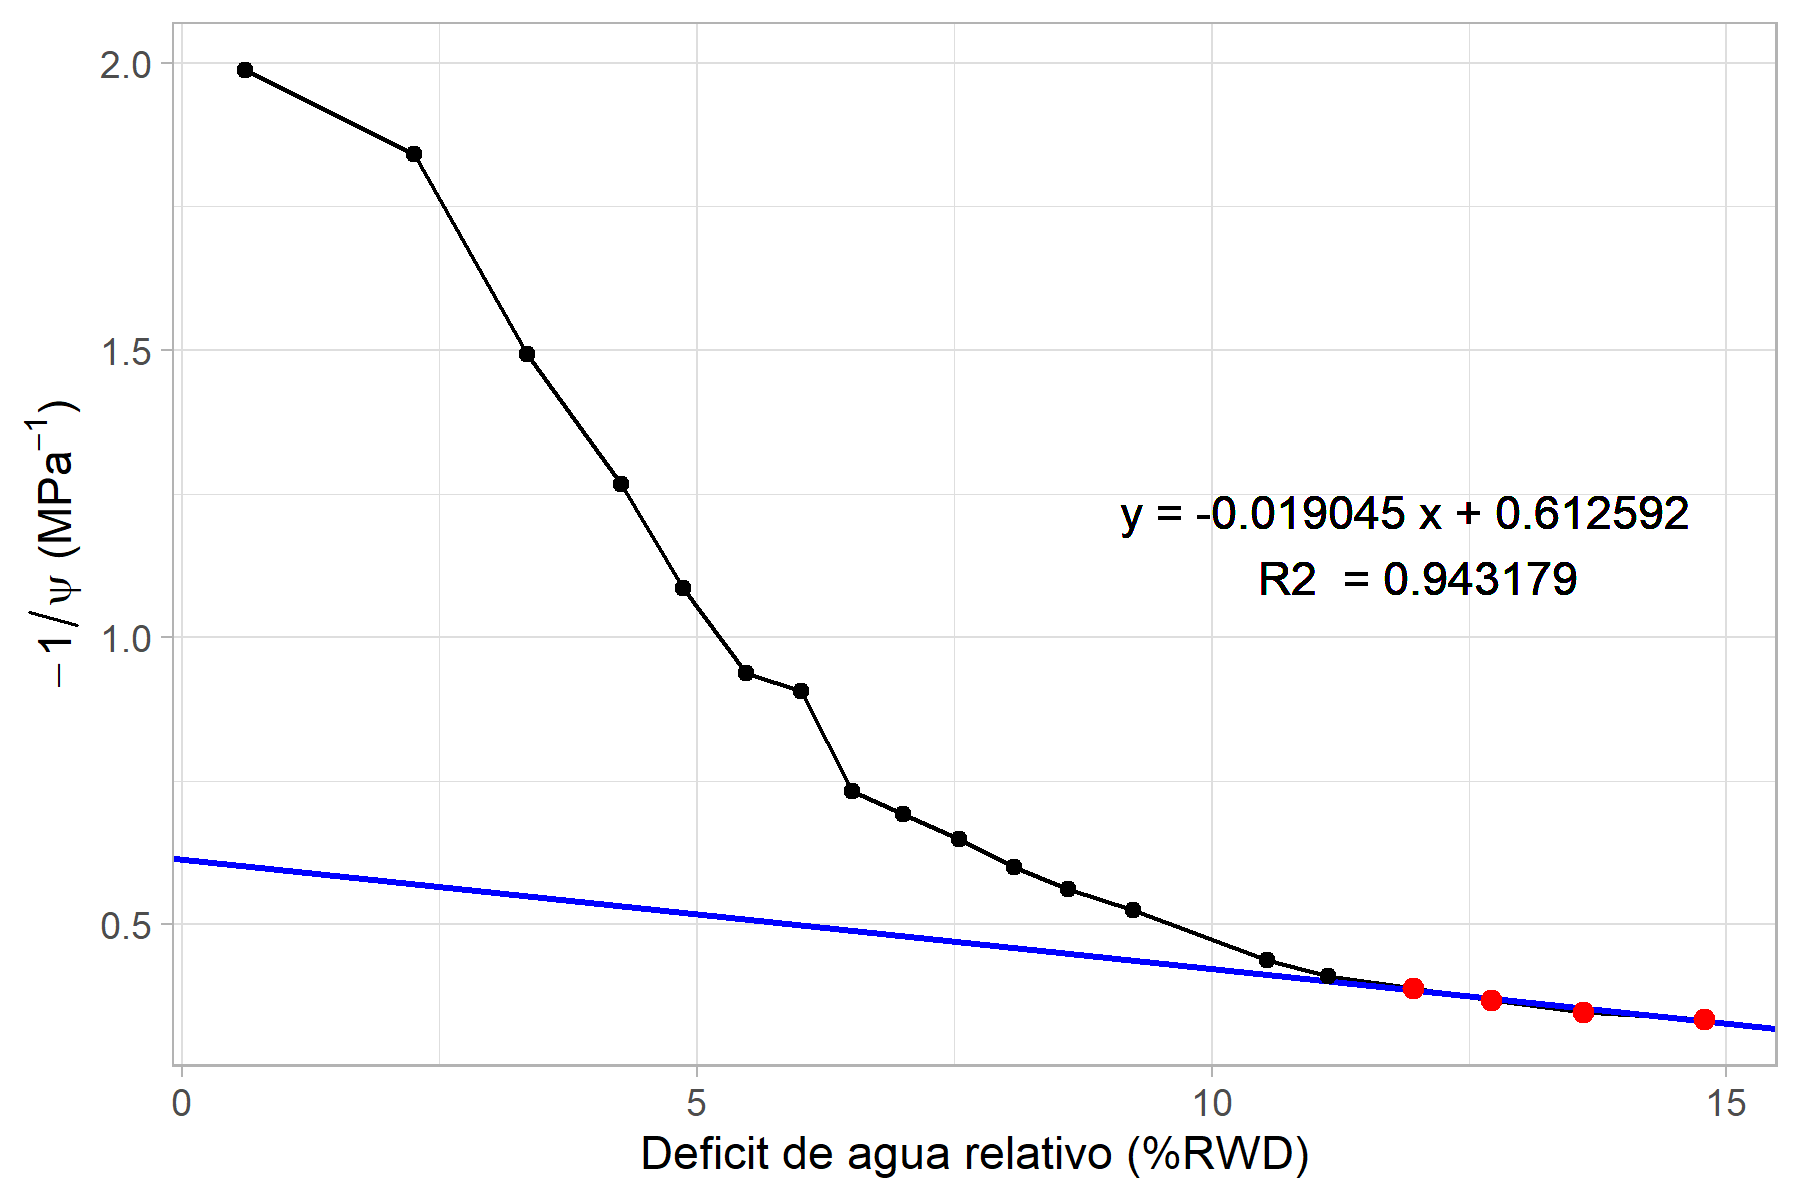
\includegraphics{figuras/06_tlp/tlp_rio_claro_T1_1.png}

Unidad 2 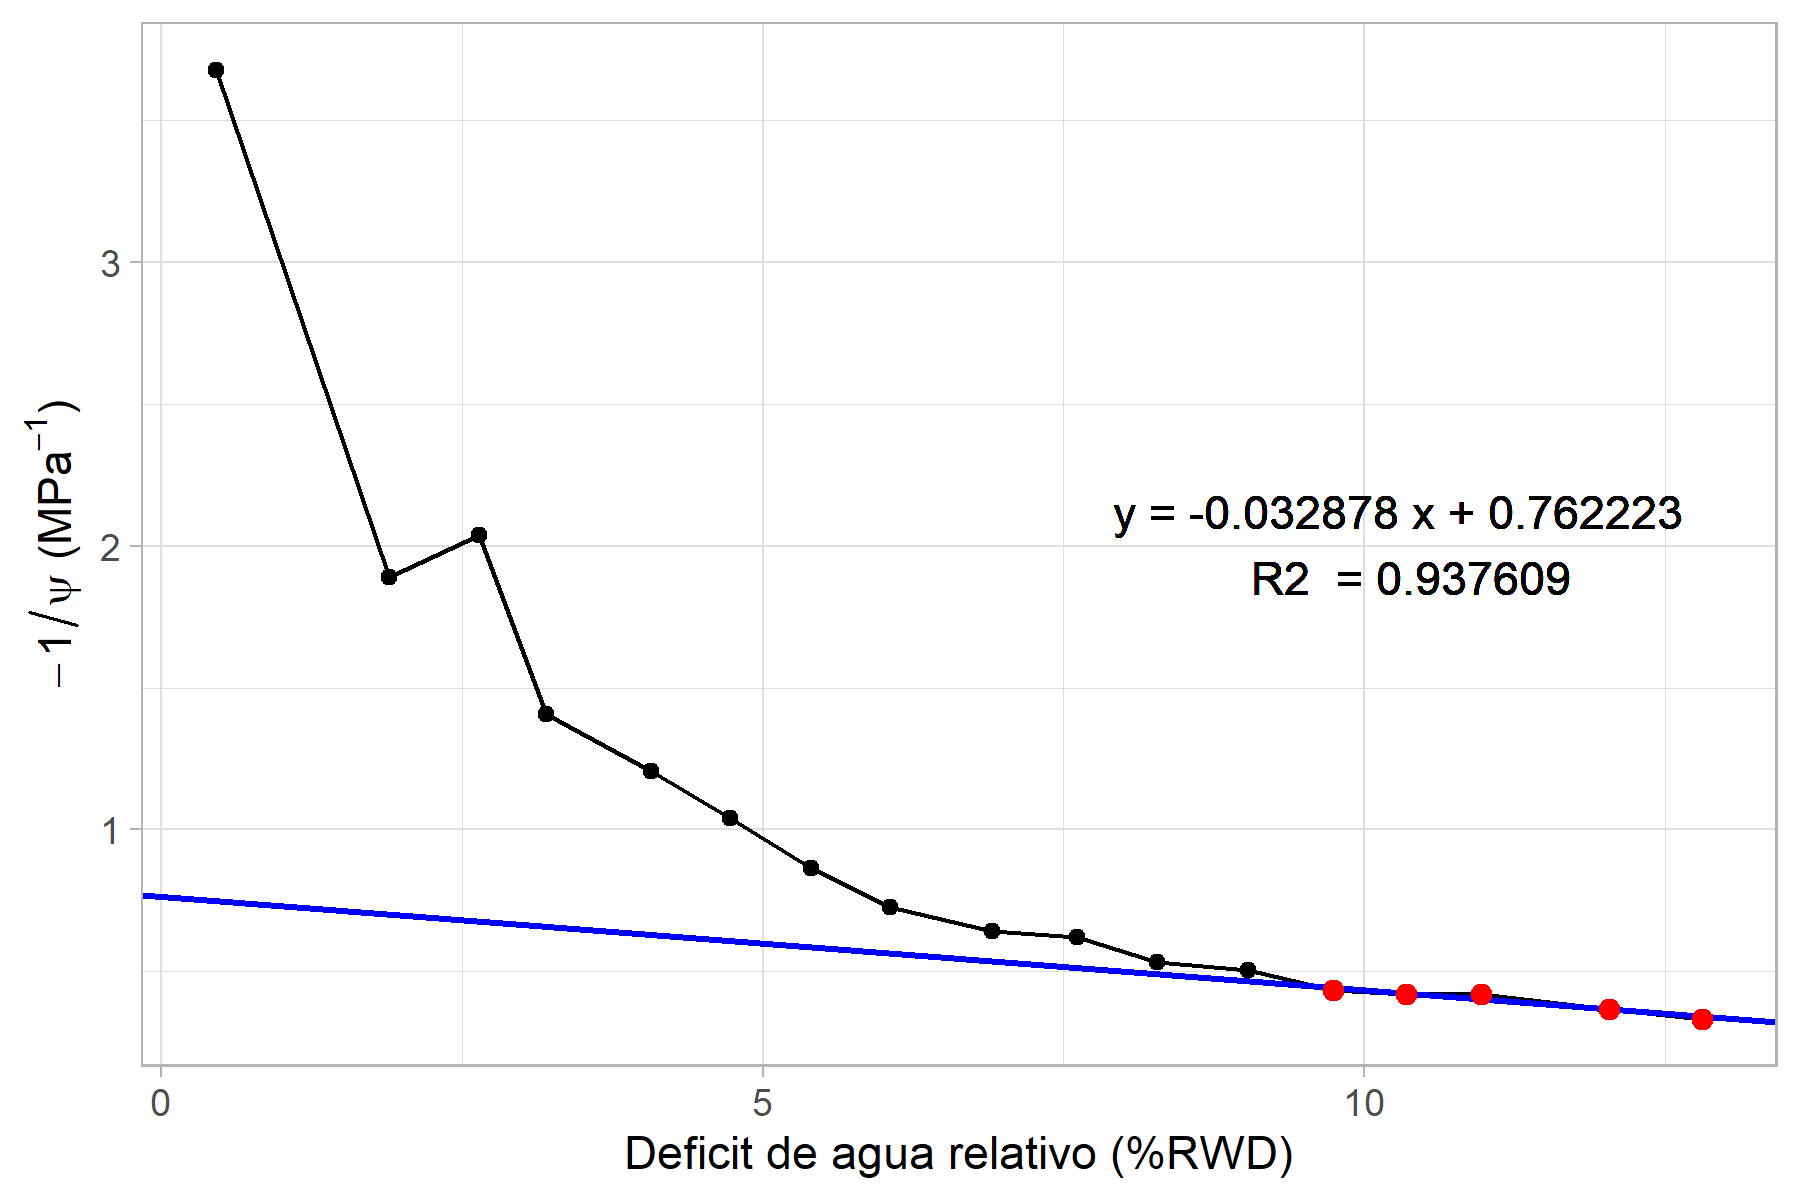
\includegraphics{figuras/06_tlp/tlp_rio_claro_T1_2.png}

Unidad 3 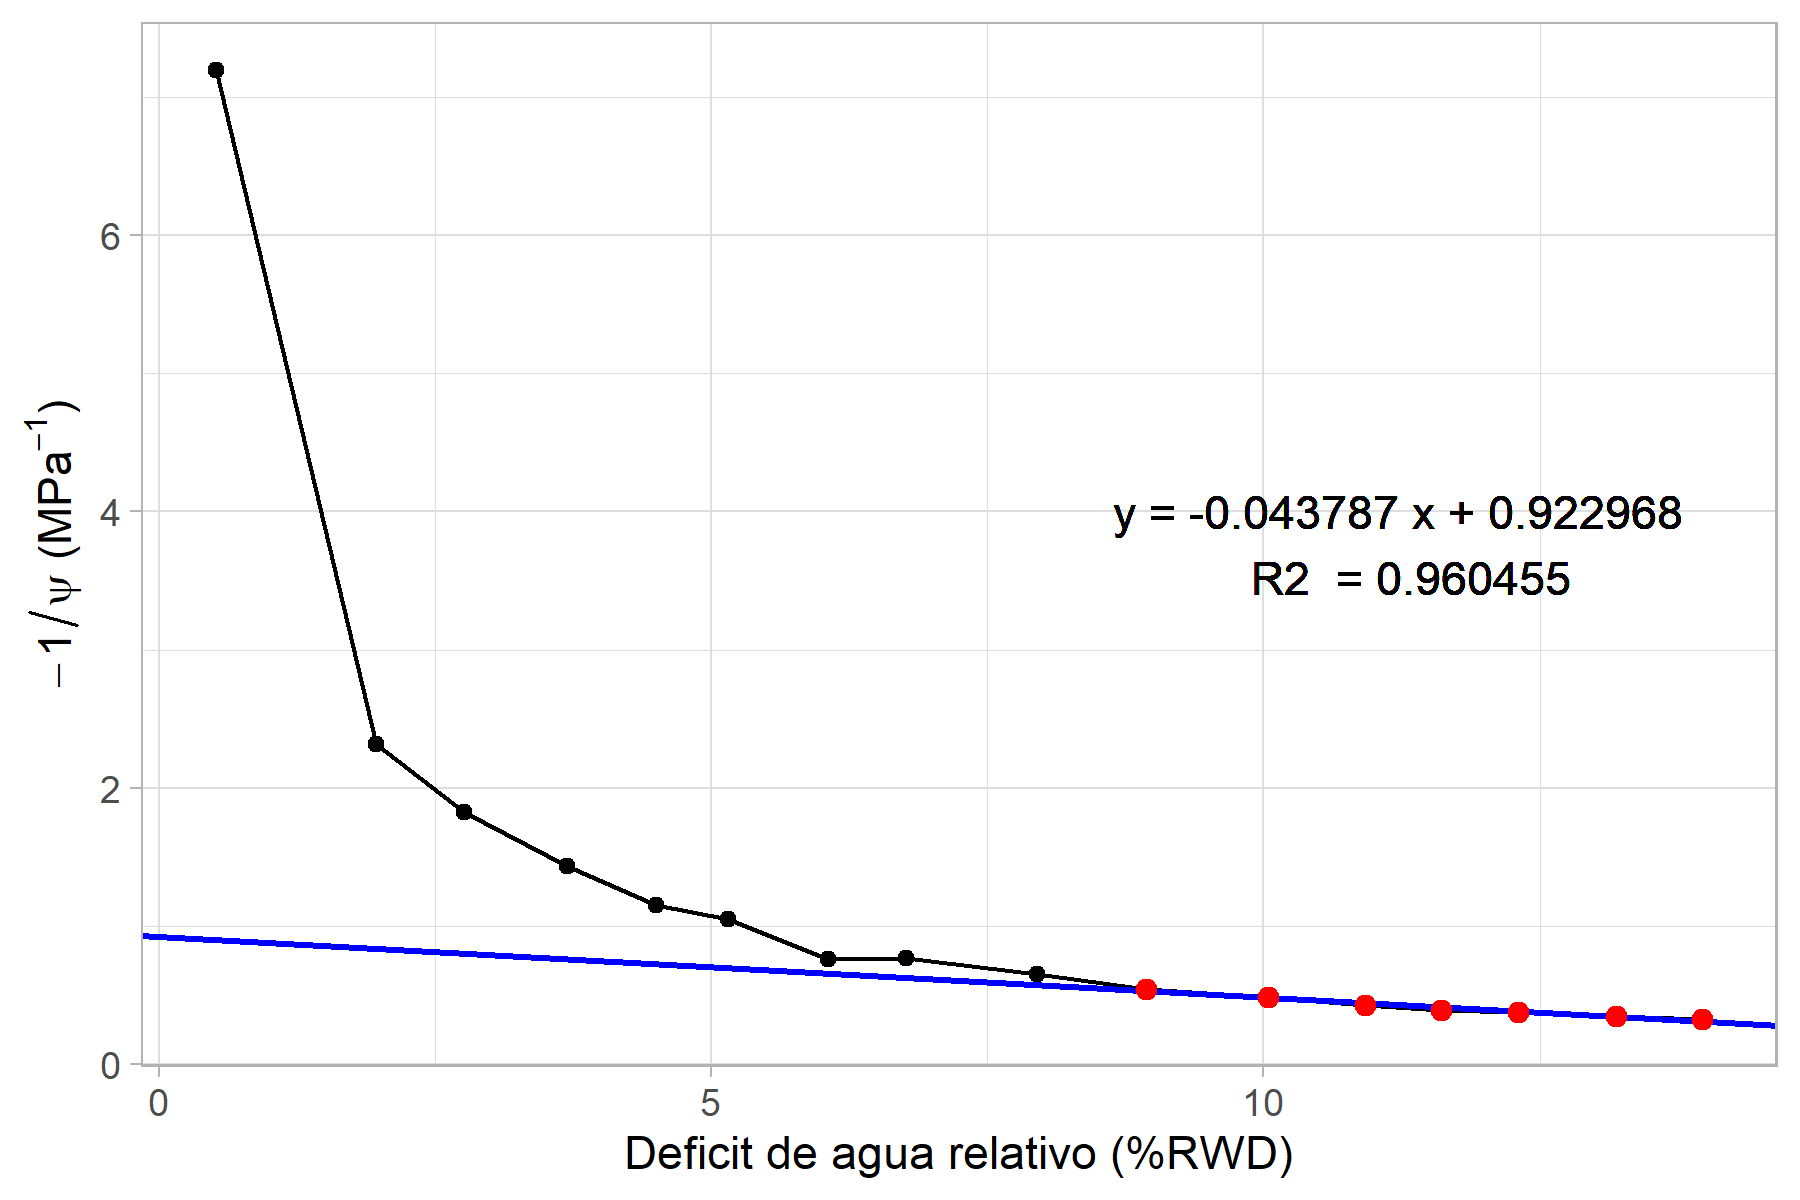
\includegraphics{figuras/06_tlp/tlp_rio_claro_T1_3.png}

\chapter{Tratamiento 2}

Unidad 1 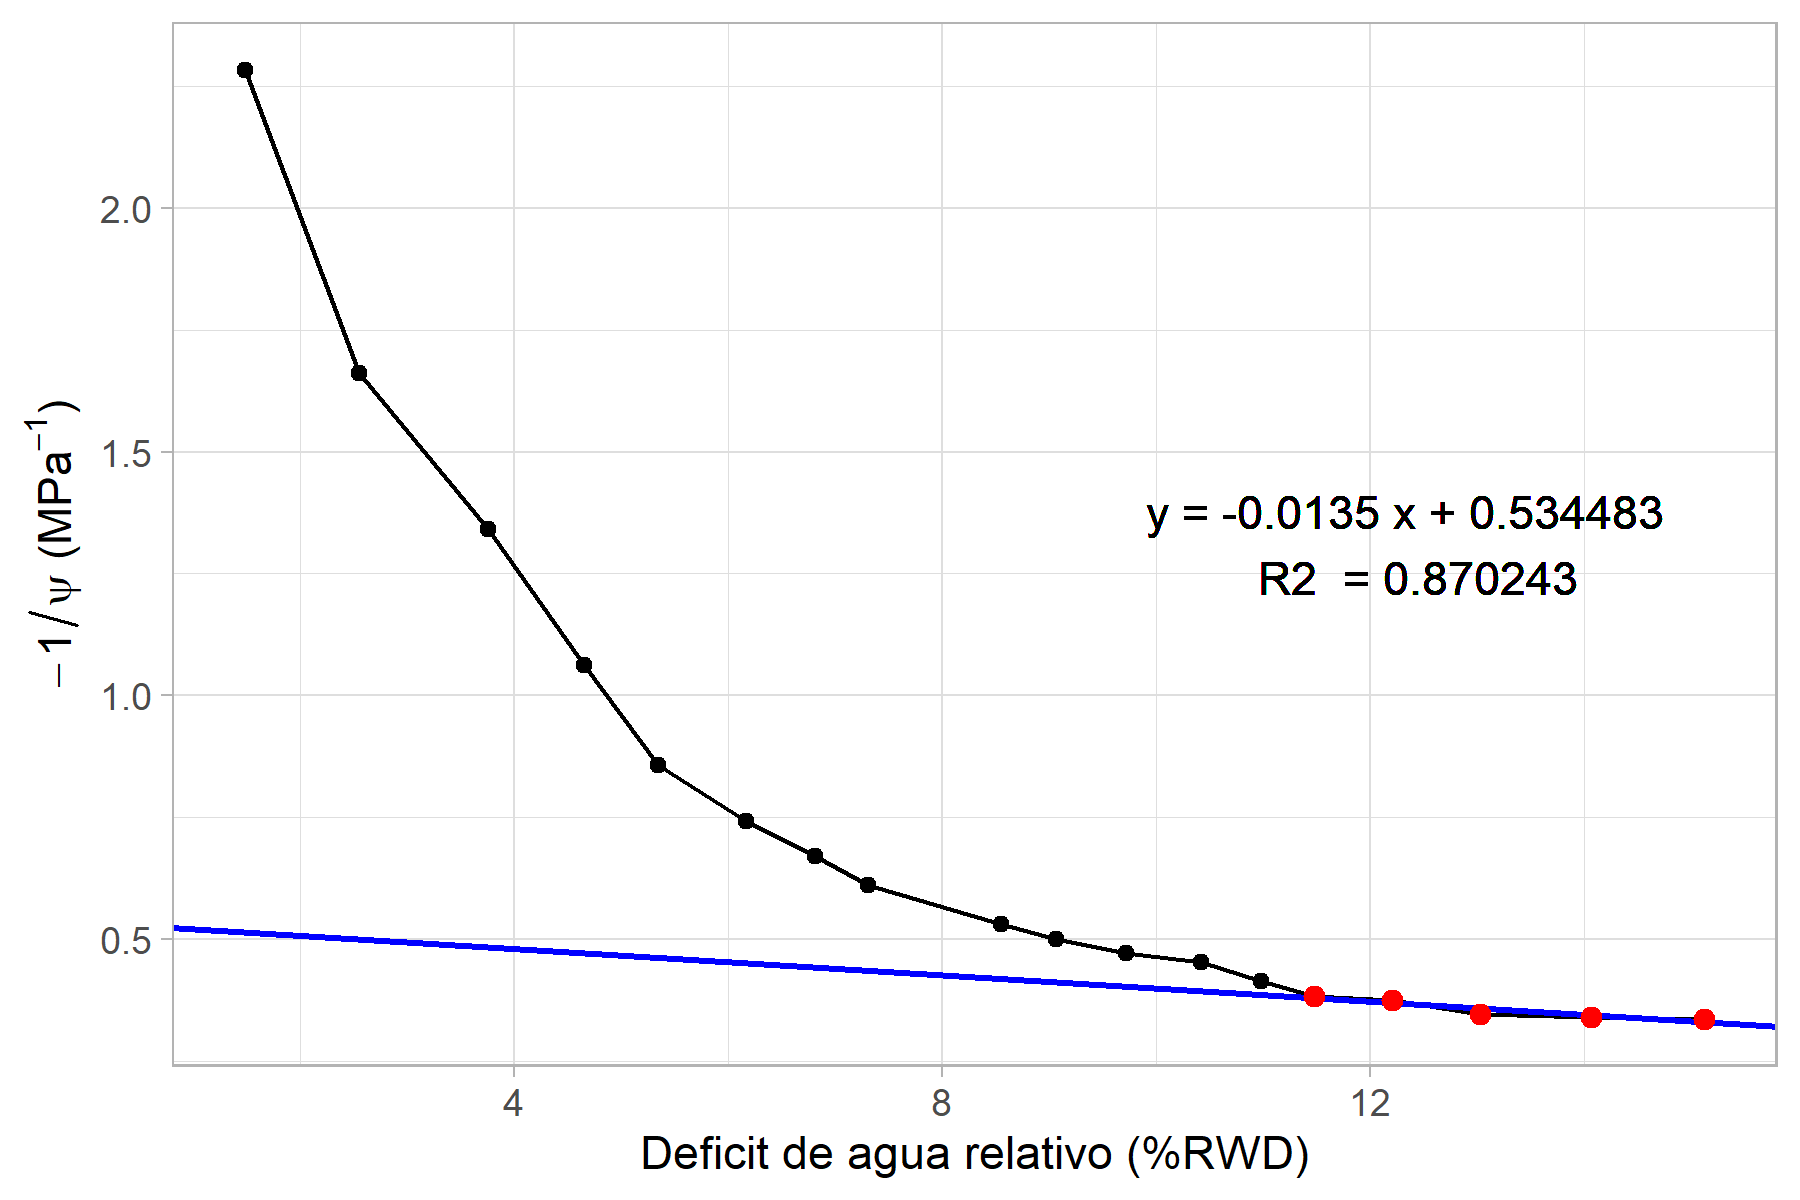
\includegraphics{figuras/06_tlp/tlp_rio_claro_T2_1.png}

Unidad 3 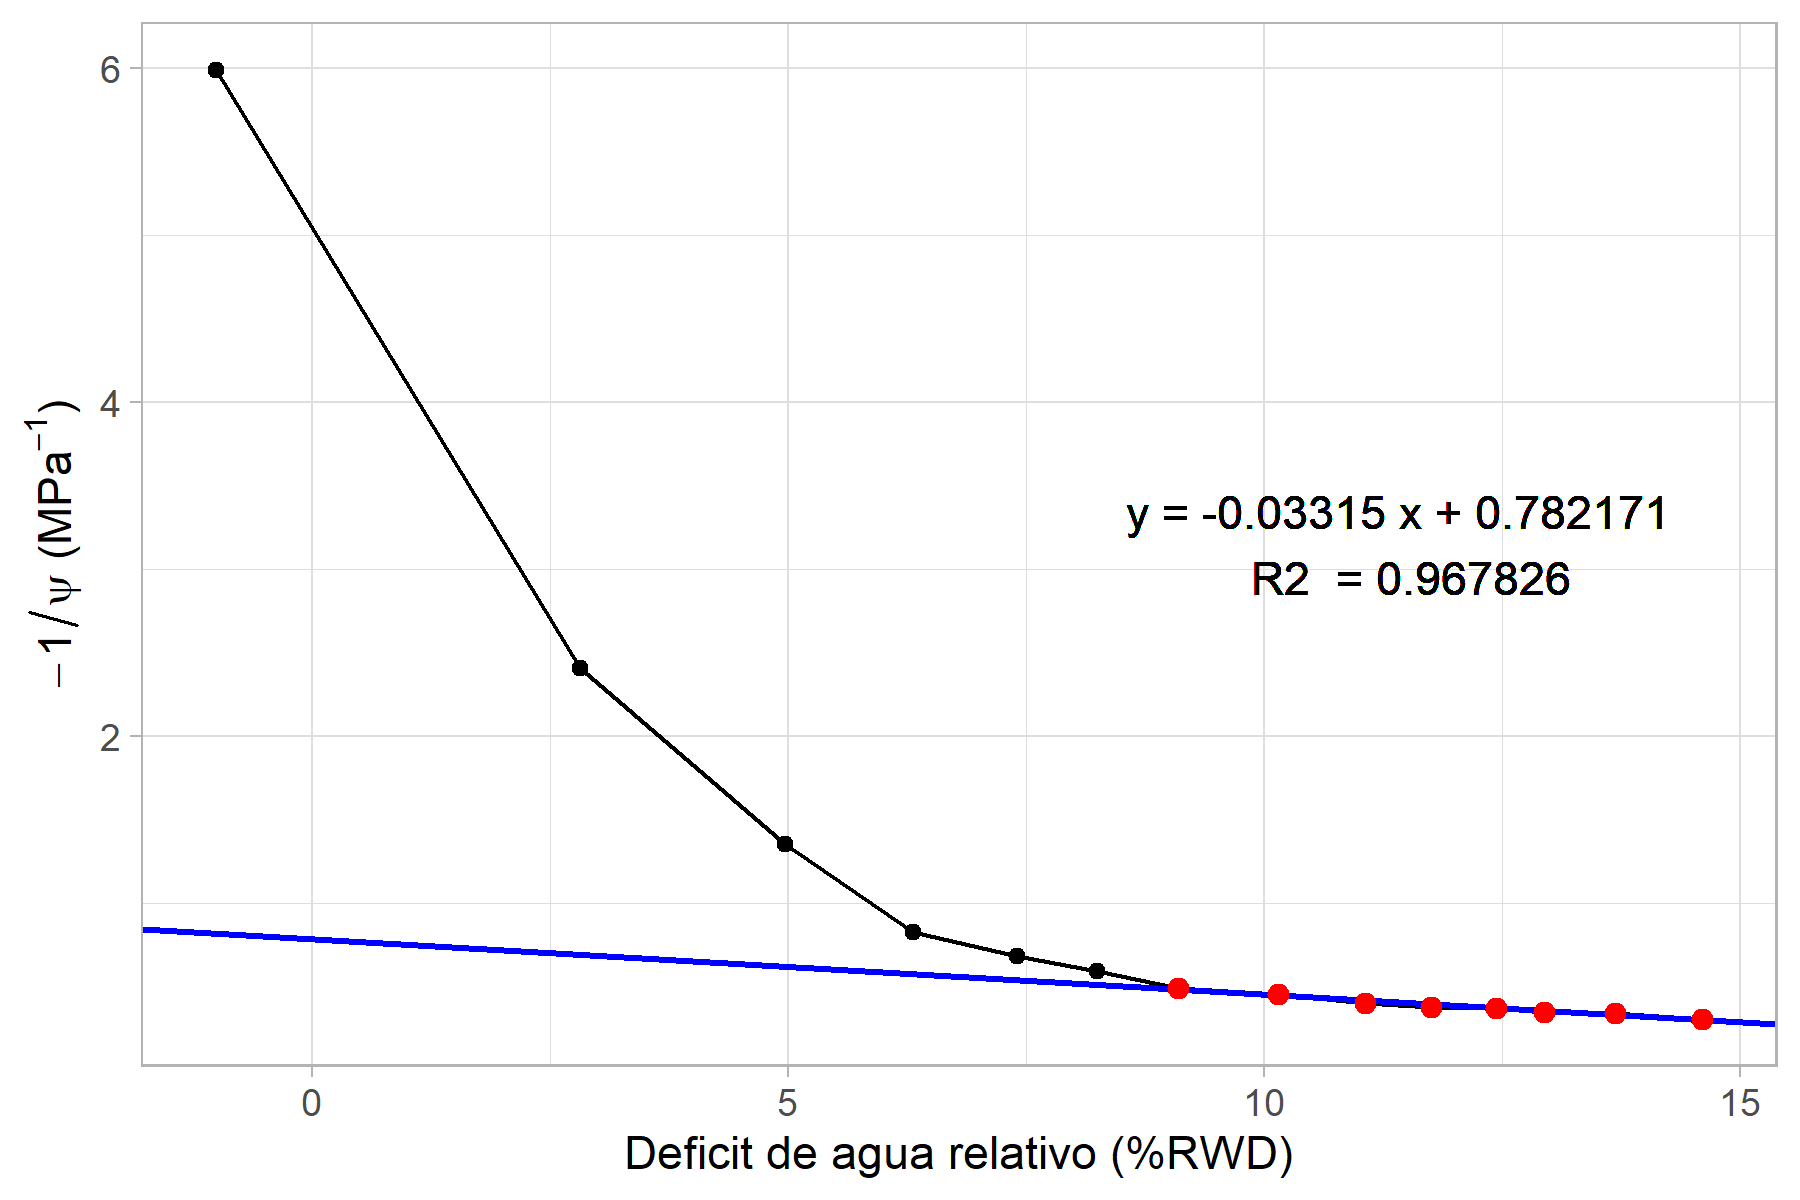
\includegraphics{figuras/06_tlp/tlp_rio_claro_T2_3.png}

\chapter{Tratamiento 3}

Unidad 1 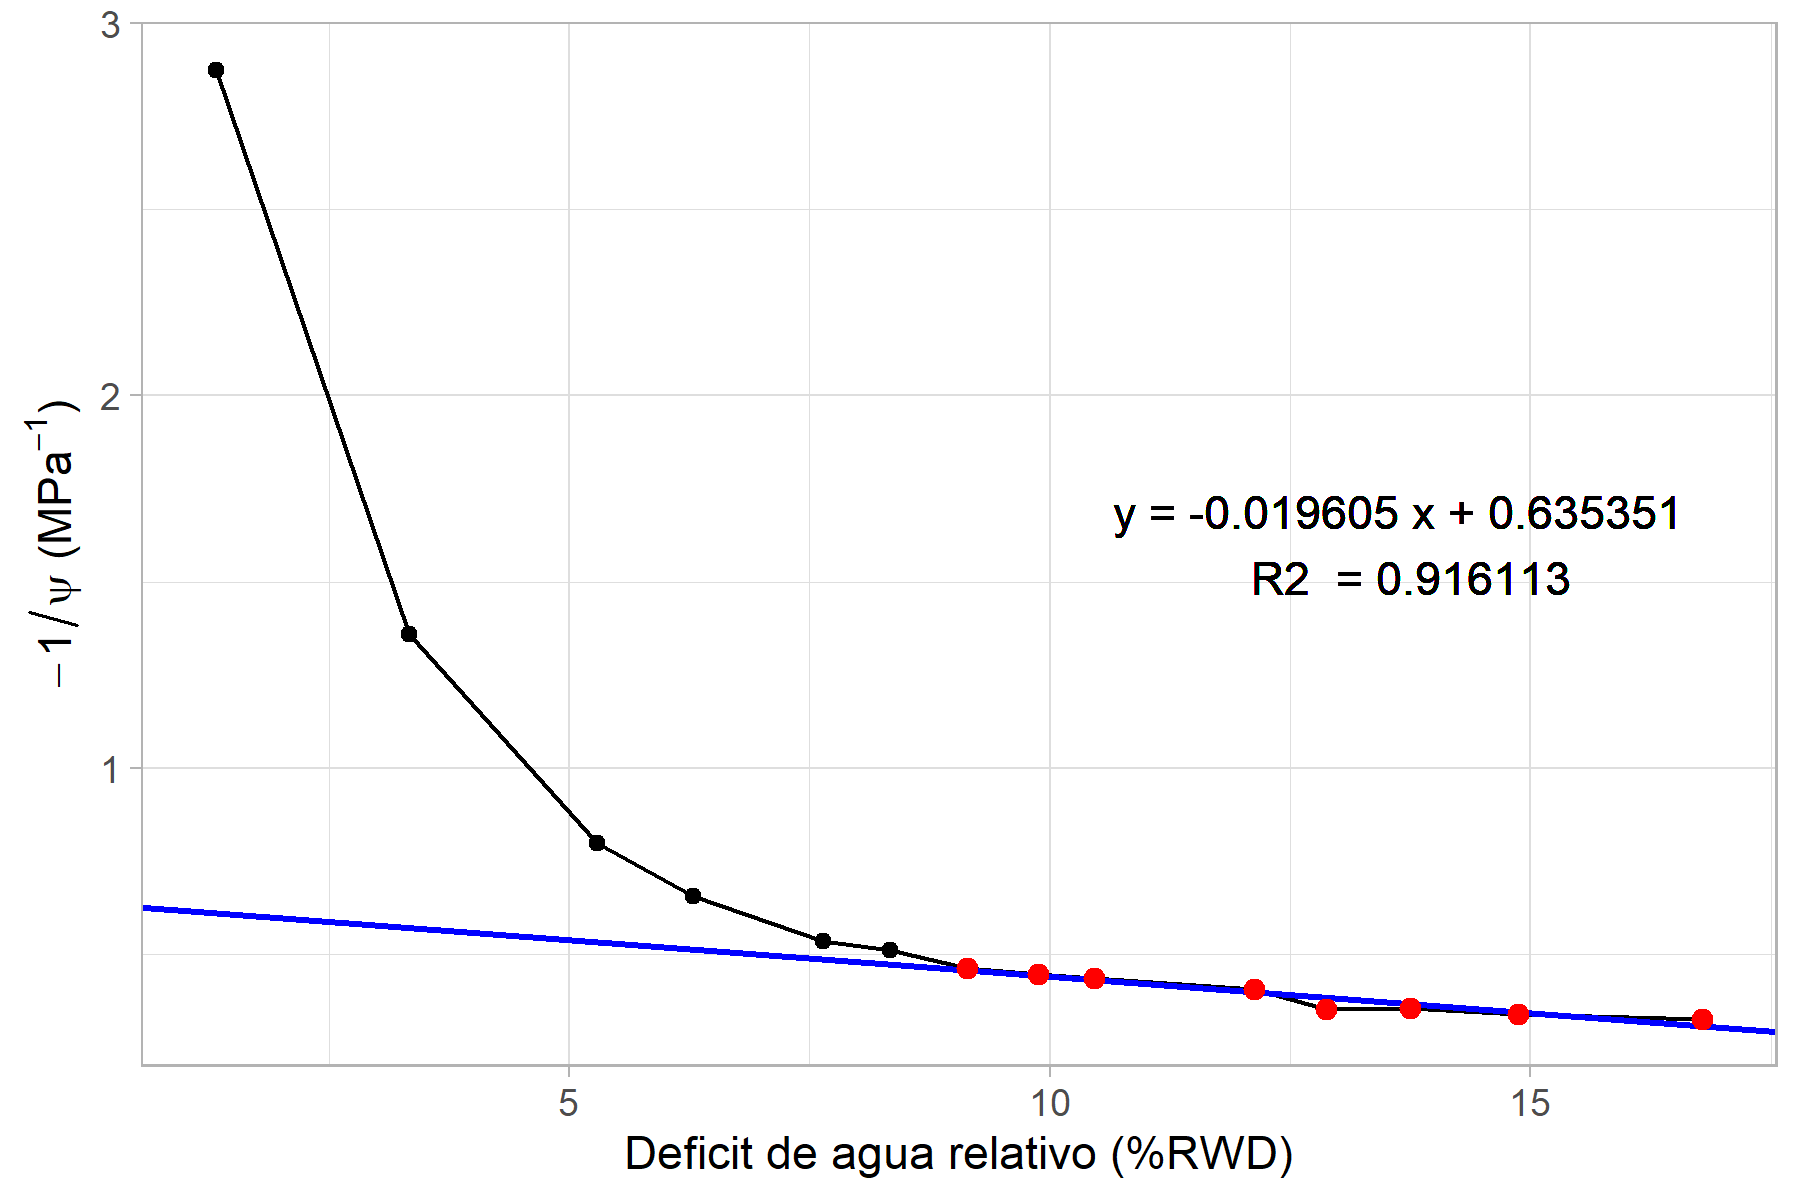
\includegraphics{figuras/06_tlp/tlp_rio_claro_T3_1.png}

Unidad 2 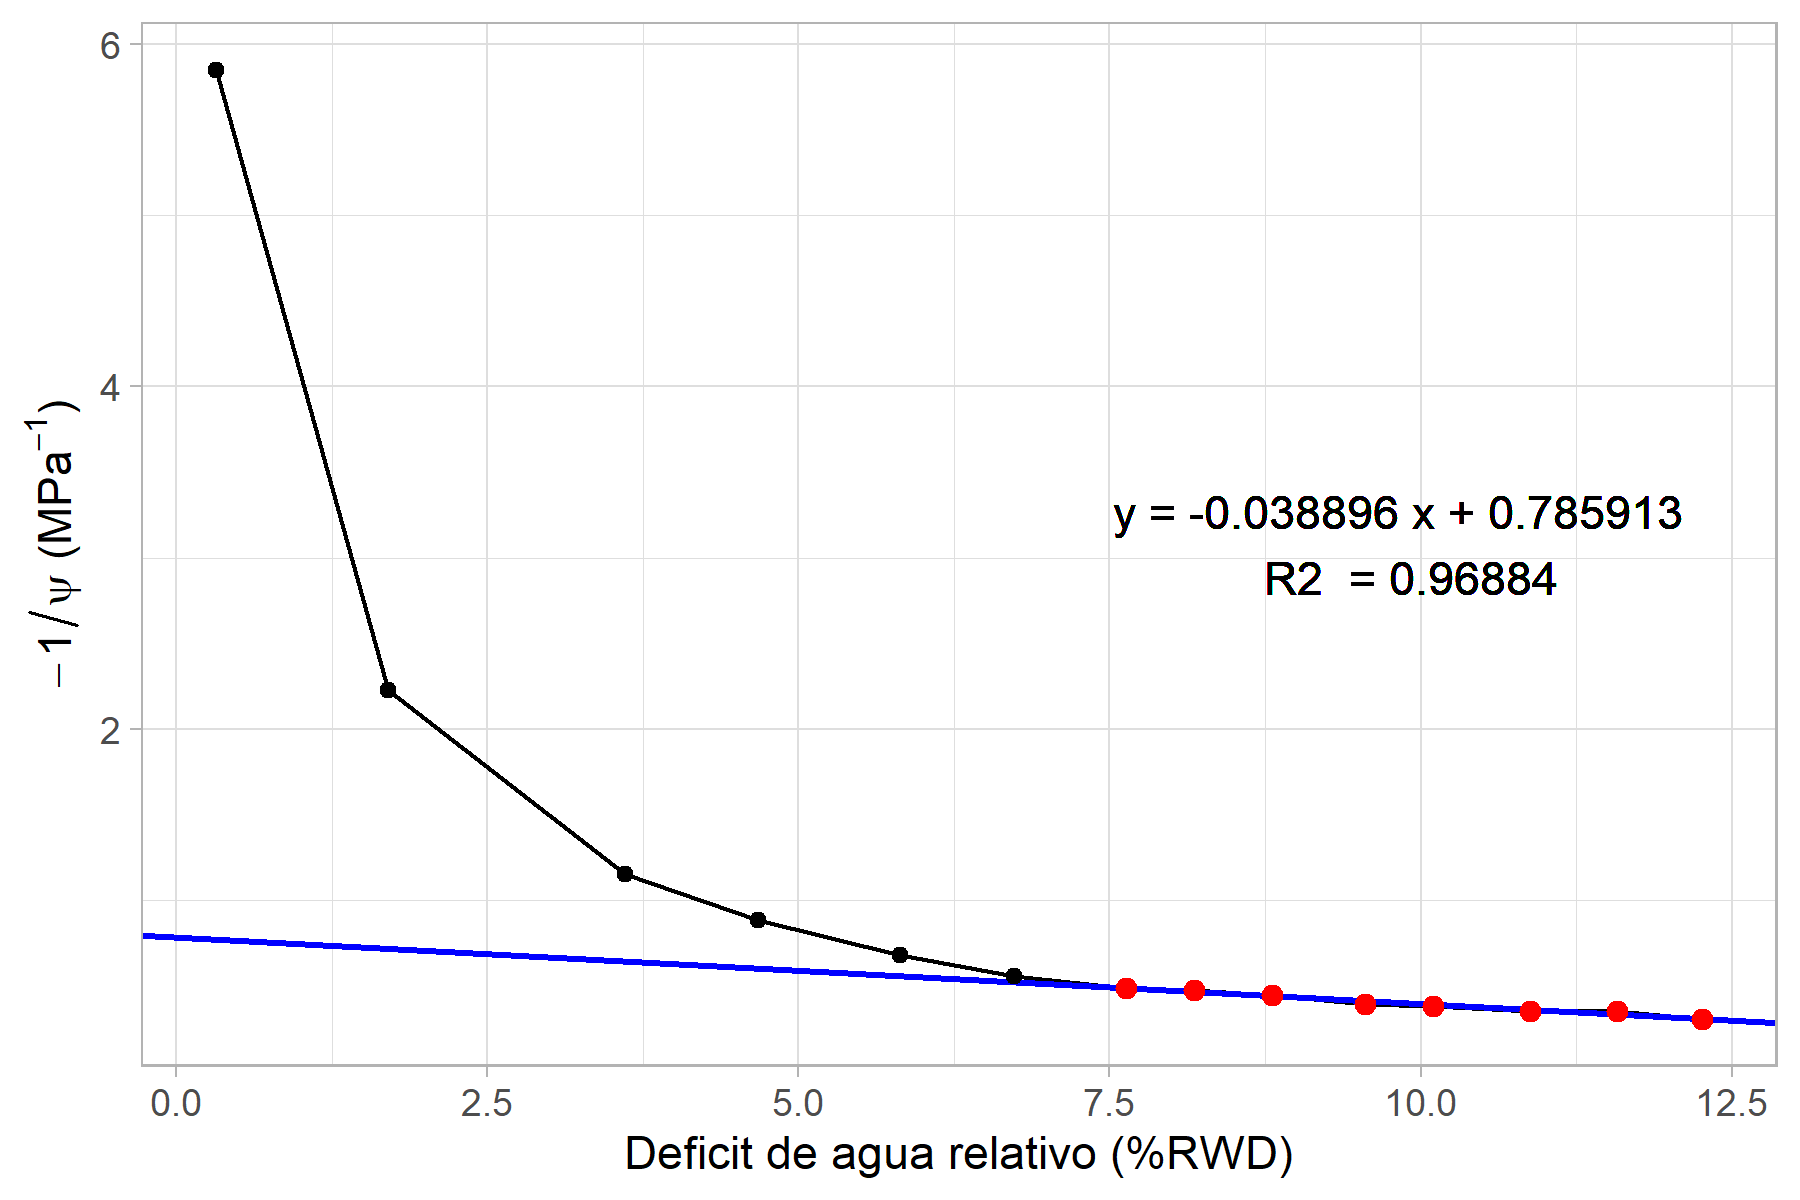
\includegraphics{figuras/06_tlp/tlp_rio_claro_T3_2.png}

Unidad 3 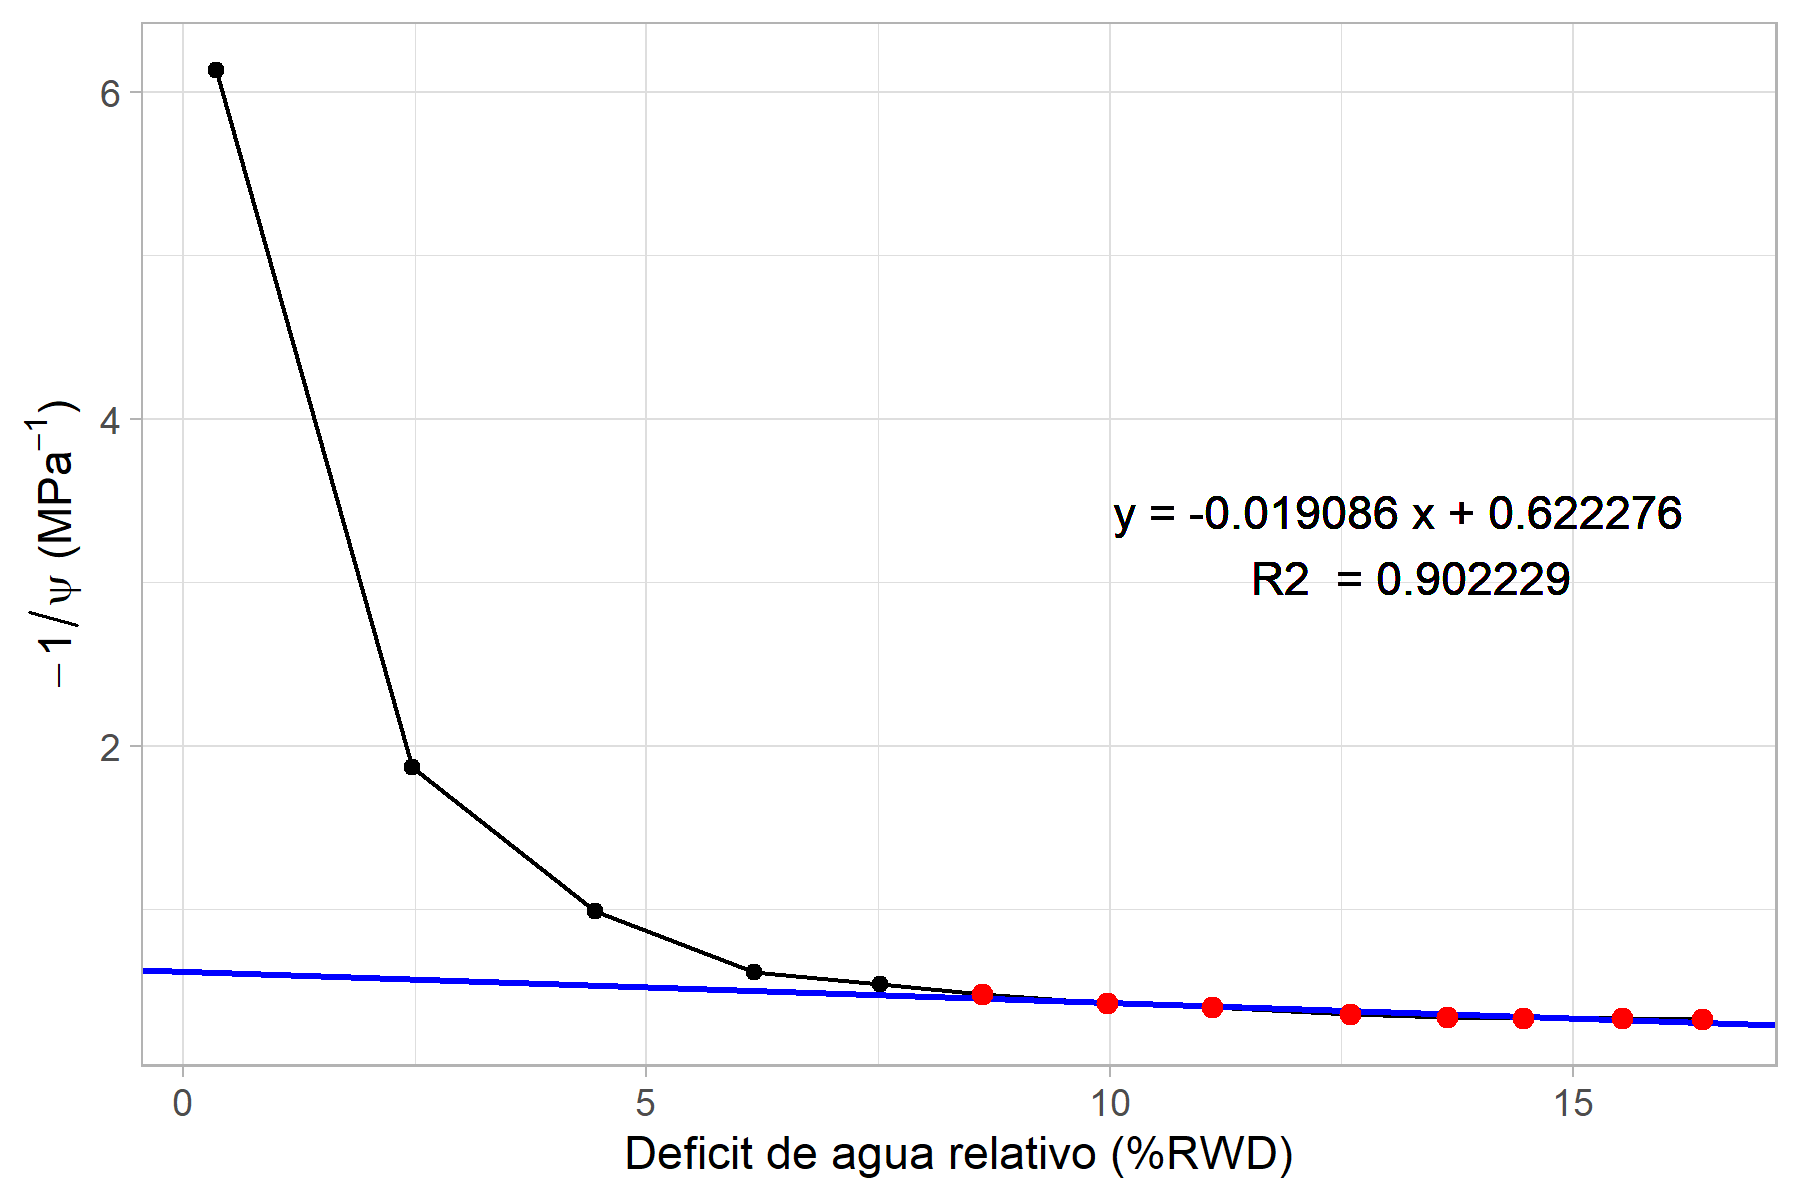
\includegraphics{figuras/06_tlp/tlp_rio_claro_T3_3.png}

\chapter{Tratamiento 4}

Unidad 1 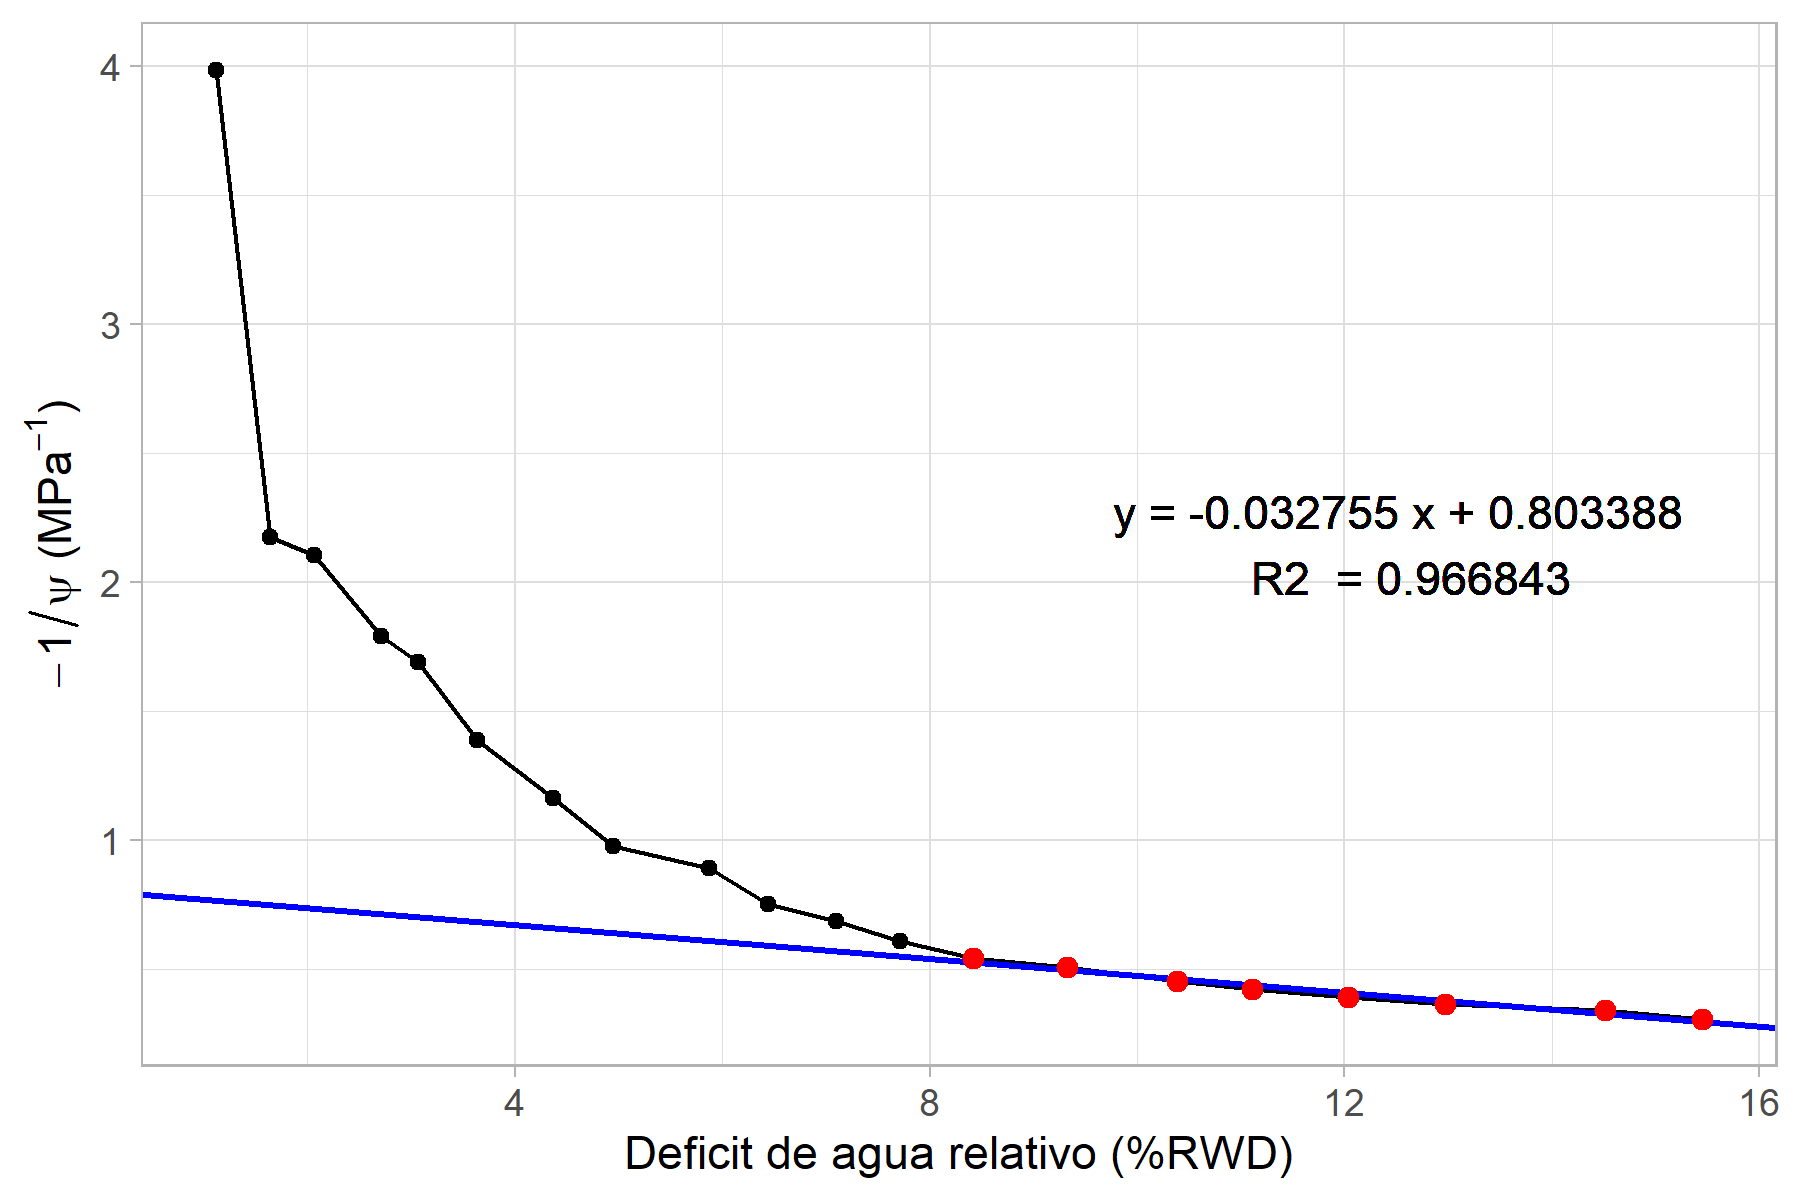
\includegraphics{figuras/06_tlp/tlp_rio_claro_T4_1.png}

Unidad 2 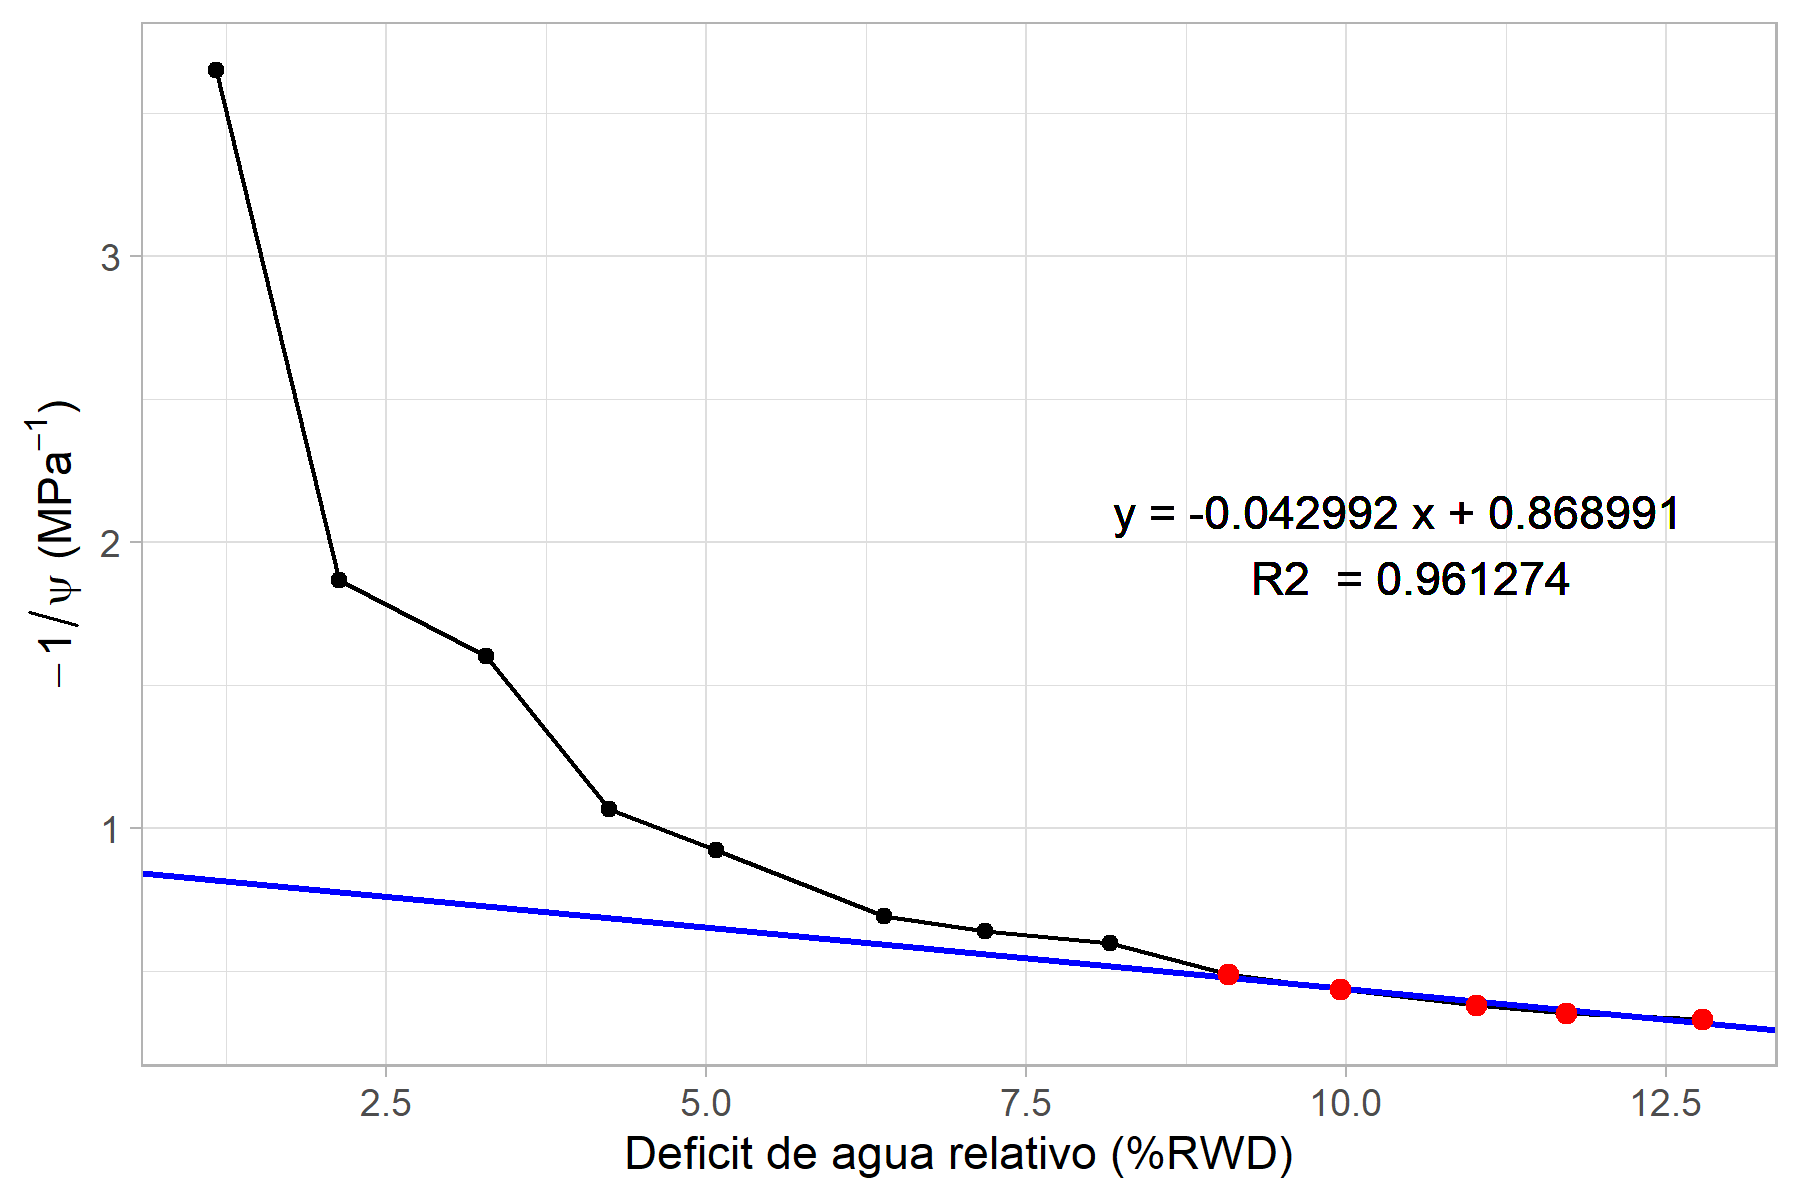
\includegraphics{figuras/06_tlp/tlp_rio_claro_T4_2.png}

Unidad 3 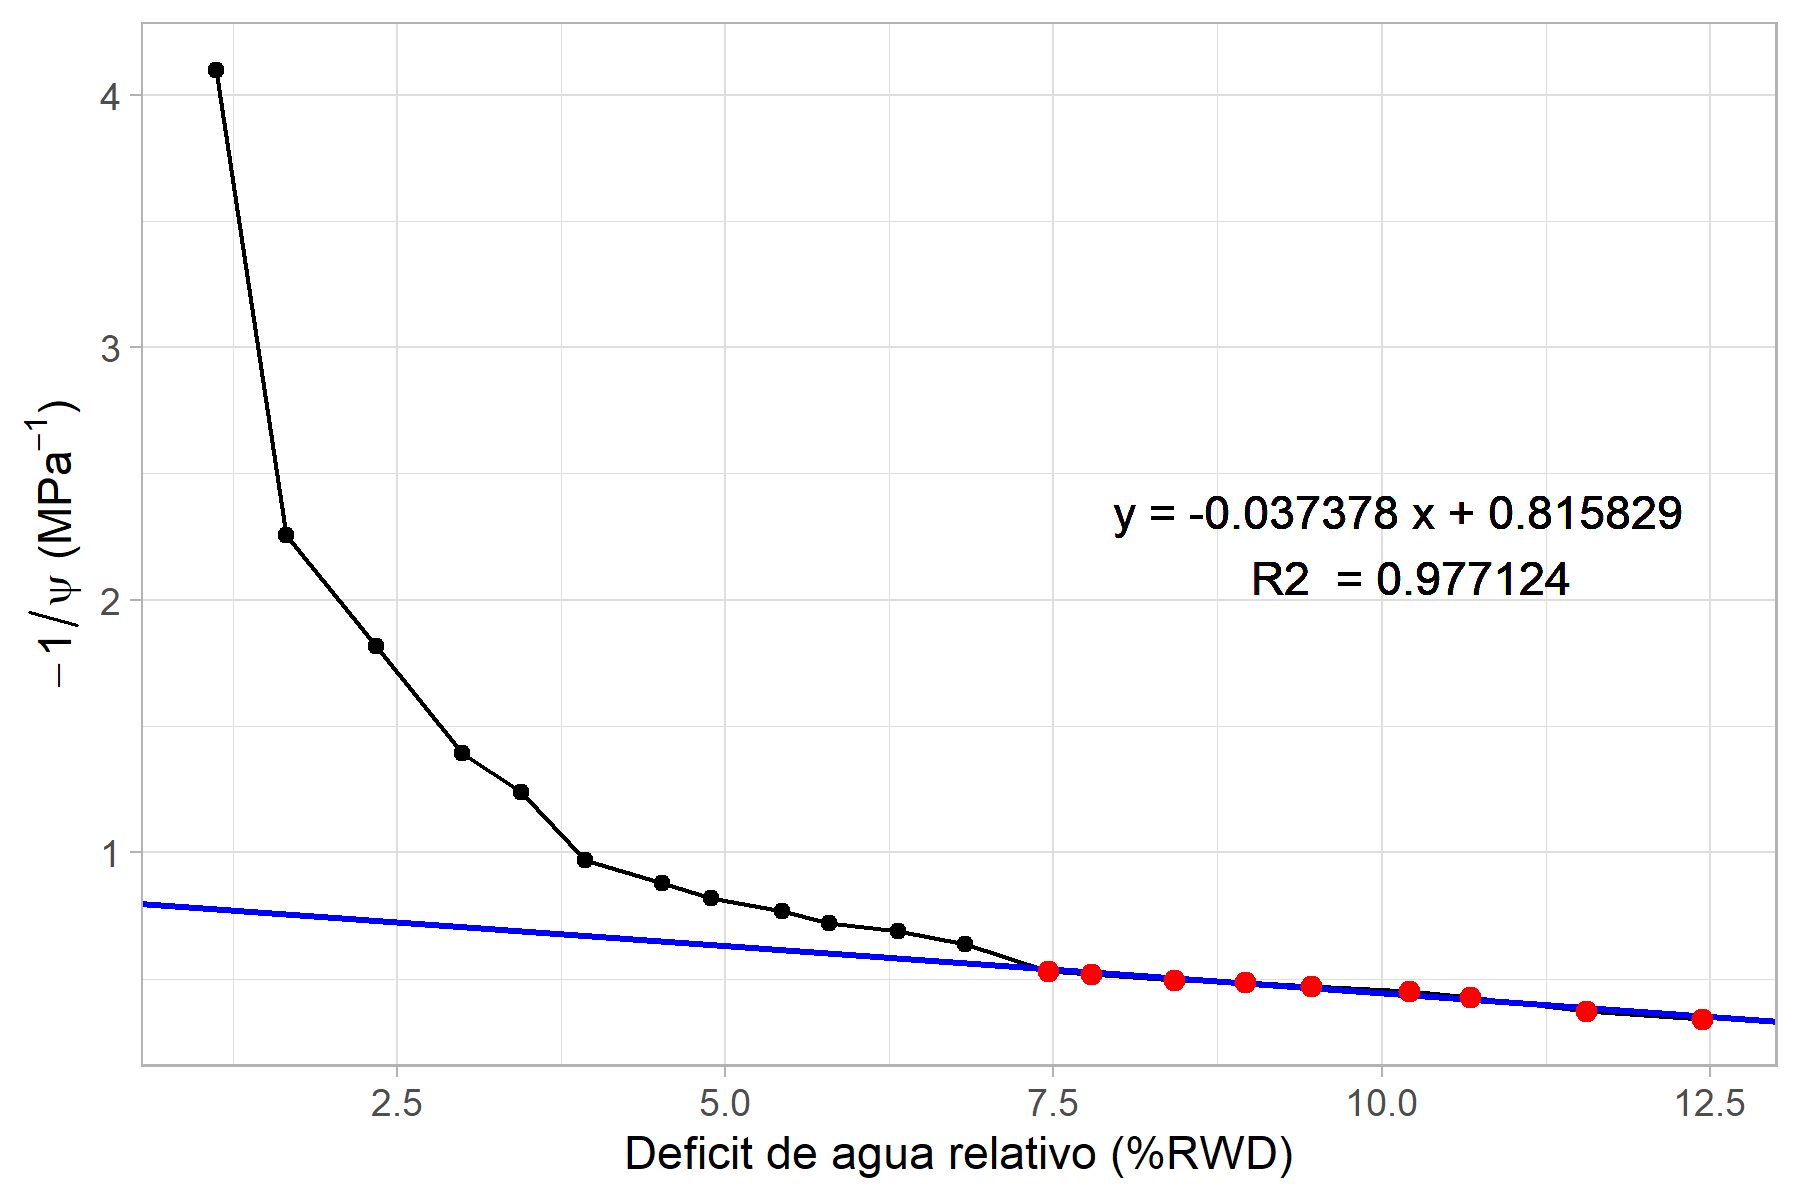
\includegraphics{figuras/06_tlp/tlp_rio_claro_T4_3.png}

\part{Capítulo 2: Preprocesamiento de datos de turgor}

Como se mencionó en la sección Sección~\ref{sec-turgor}, para el
preprocesamiento de los datos se llevó a cabo una limpieza basada en
clustering y la correlación con la temperatura y VPD. Esto permitió
diferenciar periodos que se alejaban del comportamiento normal del
turgor (i.e.~puntos máximos a la hora de más demanda hídrica del día y
disminución en las horas de la noche). A continuación se presenta el
diagrama de flujo del preprocesamiento de los datos de turgor.

\includegraphics[width=5.82in,height=7.44in]{0200_capitulo_2_files/figure-latex/mermaid-figure-1.png}

\chapter{Clustering}\label{clustering}

{[}Metodología de clustering{]}.

A continuación, se muestran las series temporales de turgor
diferenciadas por clúster, así como la distribución de las horas de
turgor mínimo y máximo para cada uno de ellos, junto con su ciclo
horario diario, abarcando todos los sensores en todas las unidades
durante las temporadas 2022-2023 y 2023-2024.

\section{La Esperanza}\label{la-esperanza-1}

\chapter{T1 (2022-2023)}

Unidad 1
\includegraphics{figuras/01_turgor_sensor/2022_2023_La_Esperanza_T1_Unidad_1.png}

Unidad 2
\includegraphics{figuras/01_turgor_sensor/2022_2023_La_Esperanza_T1_Unidad_2.png}

Unidad 3
\includegraphics{figuras/01_turgor_sensor/2022_2023_La_Esperanza_T1_Unidad_3.png}

\chapter{T2 (2022-2023)}

Unidad 1
\includegraphics{figuras/01_turgor_sensor/2022_2023_La_Esperanza_T2_Unidad_1.png}

Unidad 2
\includegraphics{figuras/01_turgor_sensor/2022_2023_La_Esperanza_T2_Unidad_2.png}

Unidad 3
\includegraphics{figuras/01_turgor_sensor/2022_2023_La_Esperanza_T2_Unidad_3.png}

\chapter{T3 (2022-2023)}

Unidad 1
\includegraphics{figuras/01_turgor_sensor/2022_2023_La_Esperanza_T3_Unidad_1.png}

Unidad 2
\includegraphics{figuras/01_turgor_sensor/2022_2023_La_Esperanza_T3_Unidad_2.png}

Unidad 3
\includegraphics{figuras/01_turgor_sensor/2022_2023_La_Esperanza_T3_Unidad_3.png}

\chapter{T4 (2022-2023)}

Unidad 1
\includegraphics{figuras/01_turgor_sensor/2022_2023_La_Esperanza_T4_Unidad_1.png}

Unidad 2
\includegraphics{figuras/01_turgor_sensor/2022_2023_La_Esperanza_T4_Unidad_2.png}

Unidad 3
\includegraphics{figuras/01_turgor_sensor/2022_2023_La_Esperanza_T4_Unidad_3.png}

\chapter{T1 (2023-2024)}

Unidad 1
\includegraphics{figuras/01_turgor_sensor/2023_2024_La_Esperanza_T1_Unidad_1.png}

Unidad 2
\includegraphics{figuras/01_turgor_sensor/2023_2024_La_Esperanza_T1_Unidad_2.png}

Unidad 3
\includegraphics{figuras/01_turgor_sensor/2023_2024_La_Esperanza_T1_Unidad_3.png}

\chapter{T2 (2023-2024)}

Unidad 1
\includegraphics{figuras/01_turgor_sensor/2023_2024_La_Esperanza_T2_Unidad_1.png}

Unidad 2
\includegraphics{figuras/01_turgor_sensor/2023_2024_La_Esperanza_T2_Unidad_2.png}

Unidad 3
\includegraphics{figuras/01_turgor_sensor/2023_2024_La_Esperanza_T2_Unidad_3.png}

\chapter{T3 (2023-2024)}

Unidad 1
\includegraphics{figuras/01_turgor_sensor/2023_2024_La_Esperanza_T3_Unidad_1.png}

Unidad 2
\includegraphics{figuras/01_turgor_sensor/2023_2024_La_Esperanza_T3_Unidad_2.png}

Unidad 3
\includegraphics{figuras/01_turgor_sensor/2023_2024_La_Esperanza_T3_Unidad_3.png}

\chapter{T4 (2023-2024)}

Unidad 1
\includegraphics{figuras/01_turgor_sensor/2023_2024_La_Esperanza_T4_Unidad_1.png}

Unidad 2
\includegraphics{figuras/01_turgor_sensor/2023_2024_La_Esperanza_T4_Unidad_2.png}

Unidad 3
\includegraphics{figuras/01_turgor_sensor/2023_2024_La_Esperanza_T4_Unidad_3.png}

\section{Rio Claro}\label{rio-claro-1}

\chapter{T1 (2022-2023)}

Unidad 1
\includegraphics{figuras/01_turgor_sensor/2022_2023_Rio_Claro_T1_Unidad_1.png}

Unidad 2
\includegraphics{figuras/01_turgor_sensor/2022_2023_Rio_Claro_T1_Unidad_2.png}

Unidad 3
\includegraphics{figuras/01_turgor_sensor/2022_2023_Rio_Claro_T1_Unidad_3.png}

\chapter{T2 (2022-2023)}

Unidad 1
\includegraphics{figuras/01_turgor_sensor/2022_2023_Rio_Claro_T2_Unidad_1.png}

Unidad 2
\includegraphics{figuras/01_turgor_sensor/2022_2023_Rio_Claro_T2_Unidad_2.png}

Unidad 3
\includegraphics{figuras/01_turgor_sensor/2022_2023_Rio_Claro_T2_Unidad_3.png}

\chapter{T3 (2022-2023)}

Unidad 1
\includegraphics{figuras/01_turgor_sensor/2022_2023_Rio_Claro_T3_Unidad_1.png}

Unidad 2
\includegraphics{figuras/01_turgor_sensor/2022_2023_Rio_Claro_T3_Unidad_2.png}

Unidad 3
\includegraphics{figuras/01_turgor_sensor/2022_2023_Rio_Claro_T3_Unidad_3.png}

\chapter{T4 (2022-2023)}

Unidad 1
\includegraphics{figuras/01_turgor_sensor/2022_2023_Rio_Claro_T4_Unidad_1.png}

Unidad 2
\includegraphics{figuras/01_turgor_sensor/2022_2023_Rio_Claro_T4_Unidad_2.png}

Unidad 3
\includegraphics{figuras/01_turgor_sensor/2022_2023_Rio_Claro_T4_Unidad_3.png}

\chapter{T1 (2023-2024)}

Unidad 1
\includegraphics{figuras/01_turgor_sensor/2023_2024_Rio_Claro_T1_Unidad_1.png}

Unidad 2
\includegraphics{figuras/01_turgor_sensor/2023_2024_Rio_Claro_T1_Unidad_2.png}

Unidad 3
\includegraphics{figuras/01_turgor_sensor/2023_2024_Rio_Claro_T1_Unidad_3.png}

\chapter{T2 (2023-2024)}

Unidad 1
\includegraphics{figuras/01_turgor_sensor/2023_2024_Rio_Claro_T2_Unidad_1.png}

Unidad 2
\includegraphics{figuras/01_turgor_sensor/2023_2024_Rio_Claro_T2_Unidad_2.png}

Unidad 3
\includegraphics{figuras/01_turgor_sensor/2023_2024_Rio_Claro_T2_Unidad_3.png}

\chapter{T3 (2023-2024)}

Unidad 1
\includegraphics{figuras/01_turgor_sensor/2023_2024_Rio_Claro_T3_Unidad_1.png}

Unidad 2
\includegraphics{figuras/01_turgor_sensor/2023_2024_Rio_Claro_T3_Unidad_2.png}

Unidad 3
\includegraphics{figuras/01_turgor_sensor/2023_2024_Rio_Claro_T3_Unidad_3.png}

\chapter{T4 (2023-2024)}

Unidad 1
\includegraphics{figuras/01_turgor_sensor/2023_2024_Rio_Claro_T4_Unidad_1.png}

Unidad 2
\includegraphics{figuras/01_turgor_sensor/2023_2024_Rio_Claro_T4_Unidad_2.png}

Unidad 3
\includegraphics{figuras/01_turgor_sensor/2023_2024_Rio_Claro_T4_Unidad_3.png}

\chapter{Limpieza de datos: eliminación de
clusters}\label{limpieza-de-datos-eliminaciuxf3n-de-clusters}

Para limpiar los datos de turgor, se emplearon series temporales de VPD
y temperatura provenientes de las estaciones meteorológicas de los dos
sitios de estudio. Se procedió a calcular el coeficiente de correlación
entre cada cluster y los valores de VPD y temperatura respecto al tiempo
(escala horaria) y el sitio. Se obtuvo un coeficiente de correlación
promedio en relación con ambas variables, y se estableció un umbral de
corte de r \textgreater{} 0.5. Aquellos clusters de turgor cuyo promedio
de correlación resultó menor a 0.5 fueron descartados.

\section{La Esperanza}\label{la-esperanza-2}

\chapter{T1 (2022-2023)}

Unidad 1
\includegraphics{figuras/02_turgor_limpiado/2022_2023_La_Esperanza_T1_Unidad_1.png}

Unidad 2
\includegraphics{figuras/02_turgor_limpiado/2022_2023_La_Esperanza_T1_Unidad_2.png}

Unidad 3
\includegraphics{figuras/02_turgor_limpiado/2022_2023_La_Esperanza_T1_Unidad_3.png}

\chapter{T2 (2022-2023)}

Unidad 1
\includegraphics{figuras/02_turgor_limpiado/2022_2023_La_Esperanza_T2_Unidad_1.png}

Unidad 2
\includegraphics{figuras/02_turgor_limpiado/2022_2023_La_Esperanza_T2_Unidad_2.png}

Unidad 3
\includegraphics{figuras/02_turgor_limpiado/2022_2023_La_Esperanza_T2_Unidad_3.png}

\chapter{T3 (2022-2023)}

Unidad 1
\includegraphics{figuras/02_turgor_limpiado/2022_2023_La_Esperanza_T3_Unidad_1.png}

Unidad 2
\includegraphics{figuras/02_turgor_limpiado/2022_2023_La_Esperanza_T3_Unidad_2.png}

Unidad 3
\includegraphics{figuras/02_turgor_limpiado/2022_2023_La_Esperanza_T3_Unidad_3.png}

\chapter{T4 (2022-2023)}

Unidad 1
\includegraphics{figuras/02_turgor_limpiado/2022_2023_La_Esperanza_T4_Unidad_1.png}

Unidad 2
\includegraphics{figuras/02_turgor_limpiado/2022_2023_La_Esperanza_T4_Unidad_2.png}

Unidad 3
\includegraphics{figuras/02_turgor_limpiado/2022_2023_La_Esperanza_T4_Unidad_3.png}

\chapter{T1 (2023-2024)}

Unidad 1
\includegraphics{figuras/02_turgor_limpiado/2023_2024_La_Esperanza_T1_Unidad_1.png}

Unidad 2
\includegraphics{figuras/02_turgor_limpiado/2023_2024_La_Esperanza_T1_Unidad_2.png}

Unidad 3
\includegraphics{figuras/02_turgor_limpiado/2023_2024_La_Esperanza_T1_Unidad_3.png}

\chapter{T2 (2023-2024)}

Unidad 1
\includegraphics{figuras/02_turgor_limpiado/2023_2024_La_Esperanza_T2_Unidad_1.png}

Unidad 2
\includegraphics{figuras/02_turgor_limpiado/2023_2024_La_Esperanza_T2_Unidad_2.png}

Unidad 3
\includegraphics{figuras/02_turgor_limpiado/2023_2024_La_Esperanza_T2_Unidad_3.png}

\chapter{T3 (2023-2024)}

Unidad 1
\includegraphics{figuras/02_turgor_limpiado/2023_2024_La_Esperanza_T3_Unidad_1.png}

Unidad 2
\includegraphics{figuras/02_turgor_limpiado/2023_2024_La_Esperanza_T3_Unidad_2.png}

Unidad 3
\includegraphics{figuras/02_turgor_limpiado/2023_2024_La_Esperanza_T3_Unidad_3.png}

\chapter{T4 (2023-2024)}

Unidad 1
\includegraphics{figuras/02_turgor_limpiado/2023_2024_La_Esperanza_T4_Unidad_1.png}

Unidad 2
\includegraphics{figuras/02_turgor_limpiado/2023_2024_La_Esperanza_T4_Unidad_2.png}

Unidad 3
\includegraphics{figuras/02_turgor_limpiado/2023_2024_La_Esperanza_T4_Unidad_3.png}

\section{Rio Claro}\label{rio-claro-2}

\chapter{T1 (2022-2023)}

Unidad 1
\includegraphics{figuras/02_turgor_limpiado/2022_2023_Rio_Claro_T1_Unidad_1.png}

Unidad 2
\includegraphics{figuras/02_turgor_limpiado/2022_2023_Rio_Claro_T1_Unidad_2.png}

Unidad 3
\includegraphics{figuras/02_turgor_limpiado/2022_2023_Rio_Claro_T1_Unidad_3.png}

\chapter{T2 (2022-2023)}

Unidad 1
\includegraphics{figuras/02_turgor_limpiado/2022_2023_Rio_Claro_T2_Unidad_1.png}

Unidad 2
\includegraphics{figuras/02_turgor_limpiado/2022_2023_Rio_Claro_T2_Unidad_2.png}

Unidad 3
\includegraphics{figuras/02_turgor_limpiado/2022_2023_Rio_Claro_T2_Unidad_3.png}

\chapter{T3 (2022-2023)}

Unidad 1
\includegraphics{figuras/02_turgor_limpiado/2022_2023_Rio_Claro_T3_Unidad_1.png}

Unidad 2
\includegraphics{figuras/02_turgor_limpiado/2022_2023_Rio_Claro_T3_Unidad_2.png}

Unidad 3
\includegraphics{figuras/02_turgor_limpiado/2022_2023_Rio_Claro_T3_Unidad_3.png}

\chapter{T4 (2022-2023)}

Unidad 1
\includegraphics{figuras/02_turgor_limpiado/2022_2023_Rio_Claro_T4_Unidad_1.png}

Unidad 2
\includegraphics{figuras/02_turgor_limpiado/2022_2023_Rio_Claro_T4_Unidad_2.png}

Unidad 3
\includegraphics{figuras/02_turgor_limpiado/2022_2023_Rio_Claro_T4_Unidad_3.png}

\chapter{T1 (2023-2024)}

Unidad 1
\includegraphics{figuras/02_turgor_limpiado/2023_2024_Rio_Claro_T1_Unidad_1.png}

Unidad 2
\includegraphics{figuras/02_turgor_limpiado/2023_2024_Rio_Claro_T1_Unidad_2.png}

Unidad 3
\includegraphics{figuras/02_turgor_limpiado/2023_2024_Rio_Claro_T1_Unidad_3.png}

\chapter{T2 (2023-2024)}

Unidad 1
\includegraphics{figuras/02_turgor_limpiado/2023_2024_Rio_Claro_T2_Unidad_1.png}

Unidad 2
\includegraphics{figuras/02_turgor_limpiado/2023_2024_Rio_Claro_T2_Unidad_2.png}

Unidad 3
\includegraphics{figuras/02_turgor_limpiado/2023_2024_Rio_Claro_T2_Unidad_3.png}

\chapter{T3 (2023-2024)}

Unidad 1
\includegraphics{figuras/02_turgor_limpiado/2023_2024_Rio_Claro_T3_Unidad_1.png}

Unidad 2
\includegraphics{figuras/02_turgor_limpiado/2023_2024_Rio_Claro_T3_Unidad_2.png}

Unidad 3
\includegraphics{figuras/02_turgor_limpiado/2023_2024_Rio_Claro_T3_Unidad_3.png}

\chapter{T4 (2023-2024)}

Unidad 1
\includegraphics{figuras/02_turgor_limpiado/2023_2024_Rio_Claro_T4_Unidad_1.png}

Unidad 2
\includegraphics{figuras/02_turgor_limpiado/2023_2024_Rio_Claro_T4_Unidad_2.png}

Unidad 3
\includegraphics{figuras/02_turgor_limpiado/2023_2024_Rio_Claro_T4_Unidad_3.png}

\chapter{Estandarización de
clusters}\label{estandarizaciuxf3n-de-clusters}

Para generar series únicas continuas por sensor (i.e.~disminuir las
discordancias entre periodos de recalibración de los sensores), se
realizó una estandarización de cada cluster, lo cual significó una
unificación las series temporales de estos a nivel de sensor. A
continuación se muestran dichas series resultantes, además de su
correlación con temperatura y VPD, y el ciclo horario del día.

\section{La Esperanza}\label{la-esperanza-3}

\chapter{T1 (2022-2023)}

Unidad 1
\includegraphics{figuras/03_turgor_union/2022_2023_La_Esperanza_T1_Unidad_1.png}

Unidad 2
\includegraphics{figuras/03_turgor_union/2022_2023_La_Esperanza_T1_Unidad_2.png}

Unidad 3
\includegraphics{figuras/03_turgor_union/2022_2023_La_Esperanza_T1_Unidad_3.png}

\chapter{T2 (2022-2023)}

Unidad 1
\includegraphics{figuras/03_turgor_union/2022_2023_La_Esperanza_T2_Unidad_1.png}

Unidad 2
\includegraphics{figuras/03_turgor_union/2022_2023_La_Esperanza_T2_Unidad_2.png}

Unidad 3
\includegraphics{figuras/03_turgor_union/2022_2023_La_Esperanza_T2_Unidad_3.png}

\chapter{T3 (2022-2023)}

Unidad 1
\includegraphics{figuras/03_turgor_union/2022_2023_La_Esperanza_T3_Unidad_1.png}

Unidad 2
\includegraphics{figuras/03_turgor_union/2022_2023_La_Esperanza_T3_Unidad_2.png}

Unidad 3
\includegraphics{figuras/03_turgor_union/2022_2023_La_Esperanza_T3_Unidad_3.png}

\chapter{T4 (2022-2023)}

Unidad 1
\includegraphics{figuras/03_turgor_union/2022_2023_La_Esperanza_T4_Unidad_1.png}

Unidad 2
\includegraphics{figuras/03_turgor_union/2022_2023_La_Esperanza_T4_Unidad_2.png}

Unidad 3
\includegraphics{figuras/03_turgor_union/2022_2023_La_Esperanza_T4_Unidad_3.png}

\chapter{T1 (2023-2024)}

Unidad 1
\includegraphics{figuras/03_turgor_union/2023_2024_La_Esperanza_T1_Unidad_1.png}

Unidad 2
\includegraphics{figuras/03_turgor_union/2023_2024_La_Esperanza_T1_Unidad_2.png}

Unidad 3
\includegraphics{figuras/03_turgor_union/2023_2024_La_Esperanza_T1_Unidad_3.png}

\chapter{T2 (2023-2024)}

Unidad 1
\includegraphics{figuras/03_turgor_union/2023_2024_La_Esperanza_T2_Unidad_1.png}

Unidad 2
\includegraphics{figuras/03_turgor_union/2023_2024_La_Esperanza_T2_Unidad_2.png}

Unidad 3
\includegraphics{figuras/03_turgor_union/2023_2024_La_Esperanza_T2_Unidad_3.png}

\chapter{T3 (2023-2024)}

Unidad 1
\includegraphics{figuras/03_turgor_union/2023_2024_La_Esperanza_T3_Unidad_1.png}

Unidad 2
\includegraphics{figuras/03_turgor_union/2023_2024_La_Esperanza_T3_Unidad_2.png}

Unidad 3
\includegraphics{figuras/03_turgor_union/2023_2024_La_Esperanza_T3_Unidad_3.png}

\chapter{T4 (2023-2024)}

Unidad 1
\includegraphics{figuras/03_turgor_union/2023_2024_La_Esperanza_T4_Unidad_1.png}

Unidad 2
\includegraphics{figuras/03_turgor_union/2023_2024_La_Esperanza_T4_Unidad_2.png}

Unidad 3
\includegraphics{figuras/03_turgor_union/2023_2024_La_Esperanza_T4_Unidad_3.png}

\section{Rio Claro}\label{rio-claro-3}

\chapter{T1 (2022-2023)}

Unidad 1
\includegraphics{figuras/03_turgor_union/2022_2023_Rio_Claro_T1_Unidad_1.png}

Unidad 2
\includegraphics{figuras/03_turgor_union/2022_2023_Rio_Claro_T1_Unidad_2.png}

Unidad 3
\includegraphics{figuras/03_turgor_union/2022_2023_Rio_Claro_T1_Unidad_3.png}

\chapter{T2 (2022-2023)}

Unidad 1
\includegraphics{figuras/03_turgor_union/2022_2023_Rio_Claro_T2_Unidad_1.png}

Unidad 2
\includegraphics{figuras/03_turgor_union/2022_2023_Rio_Claro_T2_Unidad_2.png}

Unidad 3
\includegraphics{figuras/03_turgor_union/2022_2023_Rio_Claro_T2_Unidad_3.png}

\chapter{T3 (2022-2023)}

Unidad 1
\includegraphics{figuras/03_turgor_union/2022_2023_Rio_Claro_T3_Unidad_1.png}

Unidad 2
\includegraphics{figuras/03_turgor_union/2022_2023_Rio_Claro_T3_Unidad_2.png}

Unidad 3
\includegraphics{figuras/03_turgor_union/2022_2023_Rio_Claro_T3_Unidad_3.png}

\chapter{T4 (2022-2023)}

Unidad 1
\includegraphics{figuras/03_turgor_union/2022_2023_Rio_Claro_T4_Unidad_1.png}

Unidad 2
\includegraphics{figuras/03_turgor_union/2022_2023_Rio_Claro_T4_Unidad_2.png}

Unidad 3
\includegraphics{figuras/03_turgor_union/2022_2023_Rio_Claro_T4_Unidad_3.png}

\chapter{T1 (2023-2024)}

Unidad 1
\includegraphics{figuras/03_turgor_union/2023_2024_Rio_Claro_T1_Unidad_1.png}

Unidad 2
\includegraphics{figuras/03_turgor_union/2023_2024_Rio_Claro_T1_Unidad_2.png}

Unidad 3
\includegraphics{figuras/03_turgor_union/2023_2024_Rio_Claro_T1_Unidad_3.png}

\chapter{T2 (2023-2024)}

Unidad 1
\includegraphics{figuras/03_turgor_union/2023_2024_Rio_Claro_T2_Unidad_1.png}

Unidad 2
\includegraphics{figuras/03_turgor_union/2023_2024_Rio_Claro_T2_Unidad_2.png}

Unidad 3
\includegraphics{figuras/03_turgor_union/2023_2024_Rio_Claro_T2_Unidad_3.png}

\chapter{T3 (2023-2024)}

Unidad 1
\includegraphics{figuras/03_turgor_union/2023_2024_Rio_Claro_T3_Unidad_1.png}

Unidad 2
\includegraphics{figuras/03_turgor_union/2023_2024_Rio_Claro_T3_Unidad_2.png}

Unidad 3
\includegraphics{figuras/03_turgor_union/2023_2024_Rio_Claro_T3_Unidad_3.png}

\chapter{T4 (2023-2024)}

Unidad 1
\includegraphics{figuras/03_turgor_union/2023_2024_Rio_Claro_T4_Unidad_1.png}

Unidad 2
\includegraphics{figuras/03_turgor_union/2023_2024_Rio_Claro_T4_Unidad_2.png}

Unidad 3
\includegraphics{figuras/03_turgor_union/2023_2024_Rio_Claro_T4_Unidad_3.png}

\chapter{Datos preprocesados}\label{datos-preprocesados}

\section{A nivel de unidad}\label{a-nivel-de-unidad}

Para obtener el turgor preprocesado por árbol según tratamiento, se
promediaron las series de los sensores por cada unidad, obteniendo una
serie única para cada árbol de los tratamientos.

\subsection{La Esperanza}\label{la-esperanza-4}

\chapter{T1 (2022-2023)}

Unidad 1
\includegraphics{figuras/04_turgor_unidad/2022_2023_La_Esperanza_T1_Unidad_1.png}

Unidad 2
\includegraphics{figuras/04_turgor_unidad/2022_2023_La_Esperanza_T1_Unidad_2.png}

Unidad 3
\includegraphics{figuras/04_turgor_unidad/2022_2023_La_Esperanza_T1_Unidad_3.png}

\chapter{T2 (2022-2023)}

Unidad 1
\includegraphics{figuras/04_turgor_unidad/2022_2023_La_Esperanza_T2_Unidad_1.png}

Unidad 2
\includegraphics{figuras/04_turgor_unidad/2022_2023_La_Esperanza_T2_Unidad_2.png}

Unidad 3
\includegraphics{figuras/04_turgor_unidad/2022_2023_La_Esperanza_T2_Unidad_3.png}

\chapter{T3 (2022-2023)}

Unidad 1
\includegraphics{figuras/04_turgor_unidad/2022_2023_La_Esperanza_T3_Unidad_1.png}

Unidad 2
\includegraphics{figuras/04_turgor_unidad/2022_2023_La_Esperanza_T3_Unidad_2.png}

Unidad 3
\includegraphics{figuras/04_turgor_unidad/2022_2023_La_Esperanza_T3_Unidad_3.png}

\chapter{T4 (2022-2023)}

Unidad 1
\includegraphics{figuras/04_turgor_unidad/2022_2023_La_Esperanza_T4_Unidad_1.png}

Unidad 2
\includegraphics{figuras/04_turgor_unidad/2022_2023_La_Esperanza_T4_Unidad_2.png}

Unidad 3
\includegraphics{figuras/04_turgor_unidad/2022_2023_La_Esperanza_T4_Unidad_3.png}

\chapter{T1 (2023-2024)}

Unidad 1
\includegraphics{figuras/04_turgor_unidad/2023_2024_La_Esperanza_T1_Unidad_1.png}

Unidad 2
\includegraphics{figuras/04_turgor_unidad/2023_2024_La_Esperanza_T1_Unidad_2.png}

Unidad 3
\includegraphics{figuras/04_turgor_unidad/2023_2024_La_Esperanza_T1_Unidad_3.png}

\chapter{T2 (2023-2024)}

Unidad 1
\includegraphics{figuras/04_turgor_unidad/2023_2024_La_Esperanza_T2_Unidad_1.png}

Unidad 2
\includegraphics{figuras/04_turgor_unidad/2023_2024_La_Esperanza_T2_Unidad_2.png}

Unidad 3
\includegraphics{figuras/04_turgor_unidad/2023_2024_La_Esperanza_T2_Unidad_3.png}

\chapter{T3 (2023-2024)}

Unidad 1
\includegraphics{figuras/04_turgor_unidad/2023_2024_La_Esperanza_T3_Unidad_1.png}

Unidad 2
\includegraphics{figuras/04_turgor_unidad/2023_2024_La_Esperanza_T3_Unidad_2.png}

Unidad 3
\includegraphics{figuras/04_turgor_unidad/2023_2024_La_Esperanza_T3_Unidad_3.png}

\chapter{T4 (2023-2024)}

Unidad 1
\includegraphics{figuras/04_turgor_unidad/2023_2024_La_Esperanza_T4_Unidad_1.png}

Unidad 2
\includegraphics{figuras/04_turgor_unidad/2023_2024_La_Esperanza_T4_Unidad_2.png}

Unidad 3
\includegraphics{figuras/04_turgor_unidad/2023_2024_La_Esperanza_T4_Unidad_3.png}

\subsection{Rio Claro}\label{rio-claro-4}

\chapter{T1 (2022-2023)}

Unidad 1
\includegraphics{figuras/04_turgor_unidad/2022_2023_Rio_Claro_T1_Unidad_1.png}

Unidad 2
\includegraphics{figuras/04_turgor_unidad/2022_2023_Rio_Claro_T1_Unidad_2.png}

Unidad 3
\includegraphics{figuras/04_turgor_unidad/2022_2023_Rio_Claro_T1_Unidad_3.png}

\chapter{T2 (2022-2023)}

Unidad 1
\includegraphics{figuras/04_turgor_unidad/2022_2023_Rio_Claro_T2_Unidad_1.png}

Unidad 2
\includegraphics{figuras/04_turgor_unidad/2022_2023_Rio_Claro_T2_Unidad_2.png}

Unidad 3
\includegraphics{figuras/04_turgor_unidad/2022_2023_Rio_Claro_T2_Unidad_3.png}

\chapter{T3 (2022-2023)}

Unidad 1
\includegraphics{figuras/04_turgor_unidad/2022_2023_Rio_Claro_T3_Unidad_1.png}

Unidad 2
\includegraphics{figuras/04_turgor_unidad/2022_2023_Rio_Claro_T3_Unidad_2.png}

Unidad 3
\includegraphics{figuras/04_turgor_unidad/2022_2023_Rio_Claro_T3_Unidad_3.png}

\chapter{T4 (2022-2023)}

Unidad 1
\includegraphics{figuras/04_turgor_unidad/2022_2023_Rio_Claro_T4_Unidad_1.png}

Unidad 2
\includegraphics{figuras/04_turgor_unidad/2022_2023_Rio_Claro_T4_Unidad_2.png}

Unidad 3
\includegraphics{figuras/04_turgor_unidad/2022_2023_Rio_Claro_T4_Unidad_3.png}

\chapter{T1 (2023-2024)}

Unidad 1
\includegraphics{figuras/04_turgor_unidad/2023_2024_Rio_Claro_T1_Unidad_1.png}

Unidad 2
\includegraphics{figuras/04_turgor_unidad/2023_2024_Rio_Claro_T1_Unidad_2.png}

Unidad 3
\includegraphics{figuras/04_turgor_unidad/2023_2024_Rio_Claro_T1_Unidad_3.png}

\chapter{T2 (2023-2024)}

Unidad 1
\includegraphics{figuras/04_turgor_unidad/2023_2024_Rio_Claro_T2_Unidad_1.png}

Unidad 2
\includegraphics{figuras/04_turgor_unidad/2023_2024_Rio_Claro_T2_Unidad_2.png}

Unidad 3
\includegraphics{figuras/04_turgor_unidad/2023_2024_Rio_Claro_T2_Unidad_3.png}

\chapter{T3 (2023-2024)}

Unidad 1
\includegraphics{figuras/04_turgor_unidad/2023_2024_Rio_Claro_T3_Unidad_1.png}

Unidad 2
\includegraphics{figuras/04_turgor_unidad/2023_2024_Rio_Claro_T3_Unidad_2.png}

Unidad 3
\includegraphics{figuras/04_turgor_unidad/2023_2024_Rio_Claro_T3_Unidad_3.png}

\chapter{T4 (2023-2024)}

Unidad 1
\includegraphics{figuras/04_turgor_unidad/2023_2024_Rio_Claro_T4_Unidad_1.png}

Unidad 2
\includegraphics{figuras/04_turgor_unidad/2023_2024_Rio_Claro_T4_Unidad_2.png}

Unidad 3
\includegraphics{figuras/04_turgor_unidad/2023_2024_Rio_Claro_T4_Unidad_3.png}

\section{A nivel de tratamiento}\label{a-nivel-de-tratamiento}

Para obtener el turgor preprocesado a nivel de tratamiento, se
promediaron las series promediadas de cada unidad según tratamiento,
obteniendo una serie única para cada tratamiento de en ambos sitios.

\subsection{La Esperanza}\label{la-esperanza-5}

\chapter{T1 (2022-2023)}

\includegraphics{figuras/05_turgor_tratamiento/2022_2023_La_Esperanza_T1.png}

\chapter{T2 (2022-2023)}

\includegraphics{figuras/05_turgor_tratamiento/2022_2023_La_Esperanza_T2.png}

\chapter{T3 (2022-2023)}

\includegraphics{figuras/05_turgor_tratamiento/2022_2023_La_Esperanza_T3.png}

\chapter{T4 (2022-2023)}

\includegraphics{figuras/05_turgor_tratamiento/2022_2023_La_Esperanza_T4.png}

\chapter{T1 (2023-2024)}

\includegraphics{figuras/05_turgor_tratamiento/2023_2024_La_Esperanza_T1.png}

\chapter{T2 (2023-2024)}

\includegraphics{figuras/05_turgor_tratamiento/2023_2024_La_Esperanza_T2.png}

\chapter{T3 (2023-2024)}

\includegraphics{figuras/05_turgor_tratamiento/2023_2024_La_Esperanza_T3.png}

\chapter{T4 (2023-2024)}

\includegraphics{figuras/05_turgor_tratamiento/2023_2024_La_Esperanza_T4.png}

\subsubsection{Rio Claro}\label{rio-claro-5}

\chapter{T1 (2022-2023)}

\includegraphics{figuras/05_turgor_tratamiento/2022_2023_Rio_Claro_T1.png}

\chapter{T2 (2022-2023)}

\includegraphics{figuras/05_turgor_tratamiento/2022_2023_Rio_Claro_T2.png}

\chapter{T3 (2022-2023)}

\includegraphics{figuras/05_turgor_tratamiento/2022_2023_Rio_Claro_T3.png}

\chapter{T4 (2022-2023)}

\includegraphics{figuras/05_turgor_tratamiento/2022_2023_Rio_Claro_T4.png}

\chapter{T1 (2023-2024)}

\includegraphics{figuras/05_turgor_tratamiento/2023_2024_Rio_Claro_T1.png}

\chapter{T2 (2023-2024)}

\includegraphics{figuras/05_turgor_tratamiento/2023_2024_Rio_Claro_T2.png}

\chapter{T3 (2023-2024)}

\includegraphics{figuras/05_turgor_tratamiento/2023_2024_Rio_Claro_T3.png}

\chapter{T4 (2023-2024)}

\includegraphics{figuras/05_turgor_tratamiento/2023_2024_Rio_Claro_T4.png}

\part{Capítulo 3: Punto de pérdida de turgor}

\chapter{Punto de pérdida de
turgor}\label{punto-de-puxe9rdida-de-turgor}

A continuación se presentan los puntos de pérdida de turgor de cada
unidad, según tratamiento, sitio y temporada, a partir de las curvas
presión-volumen, como fue descrito en la sección \ref{sec-pv}.

\begin{center}
\includegraphics{0301_tlp_files/figure-pdf/unnamed-chunk-1-1.pdf}
\end{center}

\part{Capítulo 4: Análisis comparativo}

Para hallar diferencias significativas tanto a nivel de tratamiento como
de temporada en un mismo sitio, se utilizó el test de Dunn, el cual
corresponde a una prueba post-hoc del test de Kruskal-Wallis para
comparar múltiples grupos sin necesidad de que los datos posean una
distribución normal (no-paramétrica).

A nivel de tratamiento, se investigaron las diferencias entre los
distintos tratamientos aplicados en un mismo sitio y temporada. Mientras
que, a nivel de temporada, se examinaron las diferencias entre distintas
temporadas dentro del mismo sitio. Para ambos análisis se utilizó un
p-value ajustado de 0.05/2.

Para visualizar las diferencias entre grupos, se generaron letras que se
colocaron en cada boxplot. Estas letras indican los grupos de semejanza
entre sí, permitiendo una interpretación más clara y detallada de los
resultados obtenidos en el análisis estadístico.

\chapter{Producción}\label{producciuxf3n-1}

\section{Peso total}\label{peso-total-1}

\chapter{Por tratamiento}

\begin{center}
\includegraphics{0401_produccion_files/figure-pdf/unnamed-chunk-2-1.pdf}
\end{center}

\chapter{Por temporada}

\begin{center}
\includegraphics{0401_produccion_files/figure-pdf/unnamed-chunk-3-1.pdf}
\end{center}

\section{Rendimiento}\label{rendimiento-1}

\chapter{Por tratamiento}

\begin{center}
\includegraphics{0401_produccion_files/figure-pdf/unnamed-chunk-4-1.pdf}
\end{center}

\chapter{Por temporada}

\begin{center}
\includegraphics{0401_produccion_files/figure-pdf/unnamed-chunk-5-1.pdf}
\end{center}

\section{Densidad}\label{densidad-1}

\chapter{Por tratamiento}

\begin{center}
\includegraphics{0401_produccion_files/figure-pdf/unnamed-chunk-6-1.pdf}
\end{center}

\chapter{Por temporada}

\begin{center}
\includegraphics{0401_produccion_files/figure-pdf/unnamed-chunk-7-1.pdf}
\end{center}

\chapter{Calidad}\label{calidad-1}

\section{Apariencia}\label{apariencia-1}

\subsection{Peso}\label{peso-1}

\chapter{Por tratamiento}

\begin{center}
\includegraphics{0402_calidad_files/figure-pdf/unnamed-chunk-2-1.pdf}
\end{center}

\chapter{Por temporada}

\begin{center}
\includegraphics{0402_calidad_files/figure-pdf/unnamed-chunk-3-1.pdf}
\end{center}

\subsection{Diametro}\label{diametro-1}

\chapter{Por tratamiento}

\begin{center}
\includegraphics{0402_calidad_files/figure-pdf/unnamed-chunk-4-1.pdf}
\end{center}

\chapter{Por temporada}

\begin{center}
\includegraphics{0402_calidad_files/figure-pdf/unnamed-chunk-5-1.pdf}
\end{center}

\chapter{Color}\label{color-1}

\chapter{Por tratamiento}

\begin{center}
\includegraphics{0402_calidad_files/figure-pdf/unnamed-chunk-6-1.pdf}
\end{center}

\chapter{Por temporada}

\begin{center}
\includegraphics{0402_calidad_files/figure-pdf/unnamed-chunk-7-1.pdf}
\end{center}

\section{Contenido de azucar}\label{contenido-de-azucar-1}

\chapter{Por tratamiento}

\begin{center}
\includegraphics{0402_calidad_files/figure-pdf/unnamed-chunk-8-1.pdf}
\end{center}

\chapter{Por temporada}

\begin{center}
\includegraphics{0402_calidad_files/figure-pdf/unnamed-chunk-9-1.pdf}
\end{center}

\section{Daño}\label{dauxf1o-1}

\chapter{Por tratamiento}

\begin{center}
\includegraphics{0402_calidad_files/figure-pdf/unnamed-chunk-10-1.pdf}
\end{center}

\chapter{Por temporada}

\begin{center}
\includegraphics{0402_calidad_files/figure-pdf/unnamed-chunk-11-1.pdf}
\end{center}

\chapter{Parámetros fisiológicos}\label{paruxe1metros-fisioluxf3gicos-1}

\section{Fluorescencia}\label{fluorescencia-1}

\chapter{Por tratamiento}

\begin{center}
\includegraphics{0403_parametros_files/figure-pdf/unnamed-chunk-2-1.pdf}
\end{center}

\chapter{Por temporada}

\begin{center}
\includegraphics{0403_parametros_files/figure-pdf/unnamed-chunk-3-1.pdf}
\end{center}

\section{Potencial}\label{potencial-1}

\chapter{Por tratamiento}

\begin{center}
\includegraphics{0403_parametros_files/figure-pdf/unnamed-chunk-4-1.pdf}
\end{center}

\chapter{Por temporada}

\begin{center}
\includegraphics{0403_parametros_files/figure-pdf/unnamed-chunk-5-1.pdf}
\end{center}

\section{LAI}\label{lai-1}

\chapter{Por tratamiento}

\begin{center}
\includegraphics{0403_parametros_files/figure-pdf/unnamed-chunk-6-1.pdf}
\end{center}

\chapter{Por temporada}

\begin{center}
\includegraphics{0403_parametros_files/figure-pdf/unnamed-chunk-7-1.pdf}
\end{center}

\chapter{Humedad de suelo}\label{humedad-de-suelo-1}

\chapter{Por tratamiento}

\begin{center}
\includegraphics{0404_humedad_files/figure-pdf/unnamed-chunk-1-1.pdf}
\end{center}

\chapter{Por temporada}

\begin{center}
\includegraphics{0404_humedad_files/figure-pdf/unnamed-chunk-2-1.pdf}
\end{center}

\part{Capítulo 5: Modelo de potencial}

\chapter{Unidimensional: turgor}\label{unidimensional-turgor}

\bookmarksetup{startatroot}

\chapter*{References}\label{references}
\addcontentsline{toc}{chapter}{References}

\markboth{References}{References}

\phantomsection\label{refs}
\begin{CSLReferences}{1}{0}
\bibitem[\citeproctext]{ref-halbritter}
Halbritter, Aud H., Amy Eycott, Sabine Reinsch, y Hans De Boeck. 2020.
{«The handbook for standardised field and laboratory measurements in
terrestrial climate-change experiments and observational studies
(ClimEx)»}. \emph{Methods in Ecology and Evolution} 11 (1): 22-37.

\bibitem[\citeproctext]{ref-knuth84}
Knuth, Donald E. 1984. {«Literate Programming»}. \emph{Comput. J.} 27
(2): 97-111. \url{https://doi.org/10.1093/comjnl/27.2.97}.

\end{CSLReferences}



\end{document}
